\documentclass[10pt,letterpaper]{article}
\usepackage{geometry}
\geometry{margin=1in}
\usepackage{graphicx}
\usepackage[dvipsnames]{xcolor}
\usepackage{moresize}

\setlength{\parindent}{0pt}
\setlength{\parskip}{0.5em}

%make lists tighter
\usepackage{enumitem}
\setlist{nolistsep}

%reduce spacing before and after section
\usepackage{titlesec}
% reduce section, subsection, etc spacing
\usepackage{titlesec}
\titlespacing*{\section}{0pt}{0\baselineskip}{0\baselineskip}
\titlespacing*{\subsection}{0pt}{0\baselineskip}{0\baselineskip}
\titlespacing*{\subsubsection}{0pt}{0\baselineskip}{0\baselineskip}

%reduce list spacing
\usepackage{enumitem}
\setlist{nosep}

\usepackage[hidelinks]{hyperref}
\usepackage{biblatex}
\usepackage{amsmath}
\usepackage{amsfonts}
\usepackage{amssymb}
\usepackage{subcaption}
\usepackage{multirow}
\addbibresource{citations.bib}

\usepackage{booktabs}
\usepackage{setspace}


\title{Lab 3.3 - FMRI, Stat 214, Spring 2025}

% submission must not contain any of your names
% but feel free to make a version for yourself with your names on it
\author{Anonymous}
\date{May 16, 2025}

\begin{document}
\maketitle

\section{Introduction}

Understanding how the human brain processes natural language remains a central challenge in neuroscience and cognitive science. In previous phases of this project, we developed encoding models to predict voxel-level brain activity from language stimuli using fMRI data from \cite{jain2018incorporating}. In Lab 3.1, we compared Bag-of-Words, Word2Vec \cite{mikolov2013efficient}, and GloVe \cite{pennington2014glove} embeddings; in Lab 3.2, we pre-trained a custom encoder using a masked language modeling objective to generate context-aware embeddings. Across both parts, these embeddings were used as inputs to ridge regression models to predict BOLD responses across voxels, providing insight into the relationship between linguistic representations and neural activity.

In this final phase, Lab 3.3, we shift focus to \textit{fine-tuning and interpreting} a large pre-trained language model for our brain prediction task. Specifically, we begin by fine-tuning BERT \cite{devlin2019bert} on the fMRI dataset to better align its embeddings with the neural responses observed during naturalistic story listening. We also explore parameter-efficient fine-tuning strategies such as Low-Rank Adaptation (LoRA) to assess whether we can achieve similar performance gains with reduced computational overhead. These fine-tuned models are then evaluated against the previously tested approaches from Labs 3.1 and 3.2.

In addition to predictive performance, this lab introduces an interpretability dimension. Using SHAP and LIME, we analyze which input words most strongly influence the model’s predictions at well-predicted voxels. By focusing on voxels where prediction accuracy is highest, we aim to uncover linguistically meaningful features that contribute to model output. Comparing the outputs of SHAP and LIME across different stories and subsets of voxels allows us to assess the consistency and plausibility of the explanations provided, offering a new perspective on how language models—and potentially the brain—represent meaning during natural language processing.


\section{EDA}

In this section, we perform a preliminary exploratory data analysis (EDA) to develop a basic understanding of the dataset. The data consists of fMRI recordings from two subjects, each listening to 101 stories. We divide the dataset into training/validation and test sets: 75 stories (75\%) are used for training and validation, while the remaining 26 stories (25\%) are reserved for testing. All EDA, embedding, and modeling are performed solely on training/validation data.

\subsection{Stories}

The stories are stored in a "list of words" format, with each story represented as a list of individual words stripped of punctuation and spacing. Figure~\ref{fig:story_length} shows the distribution of story lengths, measured by word count, for the 75 stories in the training/validation set. The histogram reveals a roughly unimodal distribution with a slight right skew. Most stories cluster around the center, with both the mean and median at 1,893 words. This similarity suggests the skew is relatively mild. Story lengths range from 697 to 3,476 words, indicating substantial variation in stimulus duration.

\begin{figure}[ht]
    \centering
    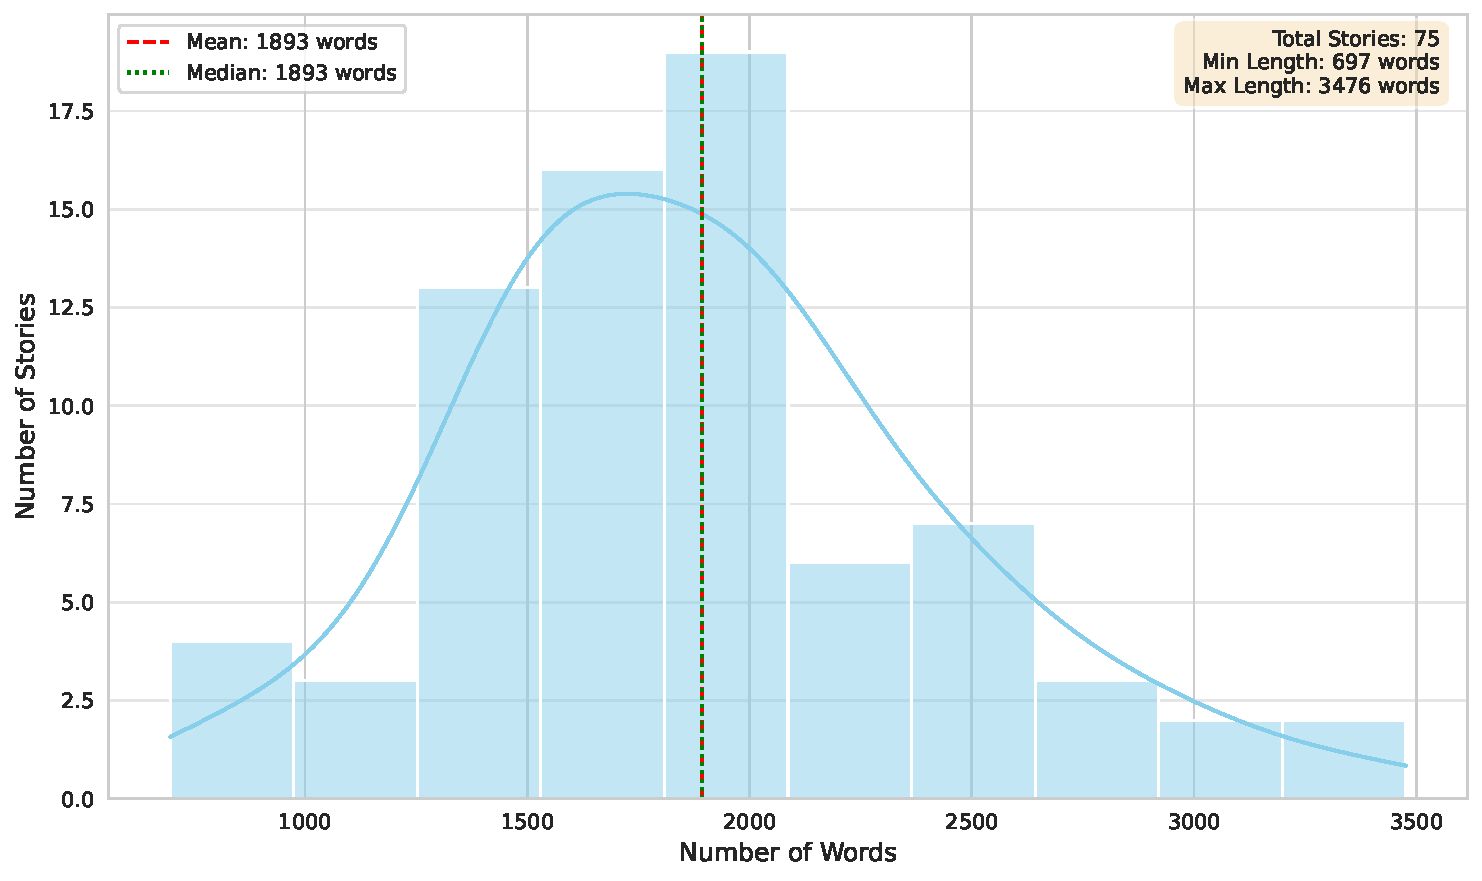
\includegraphics[width=0.8\textwidth]{figs/story_length_distribution.pdf}
    \caption{Distribution of story lengths in training/validation dataset.}
    \label{fig:story_length}
\end{figure}

The excerpt below is a sample passage from one of the stories, with punctuation added for readability, as it is not present in the original data.

\begin{quotation}
    "My story begins, I am driving my uh silver station Volvo uh from Brooklyn to my mother's house in Rosedale, Queens, on a hot mid-afternoon August day in two thousand and three. My mother uh is a widow. Uh, my father has passed away from lung cancer fifteen years before, nineteen eighty-eight, and she has not resumed dating. She has sworn off men in no uncertain terms. She has told me that, "I am never, ever going to wash another pair of men's underwear again. I am finished with the species. I'm done."
\end{quotation}

The story is a narrative piece, rich in detail and context. The language is conversational, featuring personal anecdotes and reflections. The presence of filler words like "uh" reflects natural speech patterns, suggesting that the corpus is informal and may differ from the more formal text typically used in NLP tasks.


\subsection{fMRI Signals}
The fMRI signal data capture the brain's response, measured via the Blood-Oxygen-Level-Dependent (BOLD) signal, as subjects listened to the stories. For each of the 75 stories comprising the training/validation set for a given subject, the data is organized into a two-dimensional numerical array. Each row in this array represents the brain activity across all measured voxels at a specific Time of Repetition (TR), which is the sampling interval of the fMRI scanner. Each column corresponds to a single voxel, with $94,251$ voxels for Subject 2 or $95,556$ for Subject 3, recorded per subject. Consequently, the dimensions of these arrays are \(T \times V\), where \(V\) is constant, and \(T\) (the number of TRs) varies from story to story, reflecting the differing lengths of the narratives; indeed, as shown in Figure \ref{fig:word_count}, there is a strong positive correlation between the number of words in a story and the duration of its corresponding fMRI recording in TRs.

\begin{figure}[ht]
    \centering
    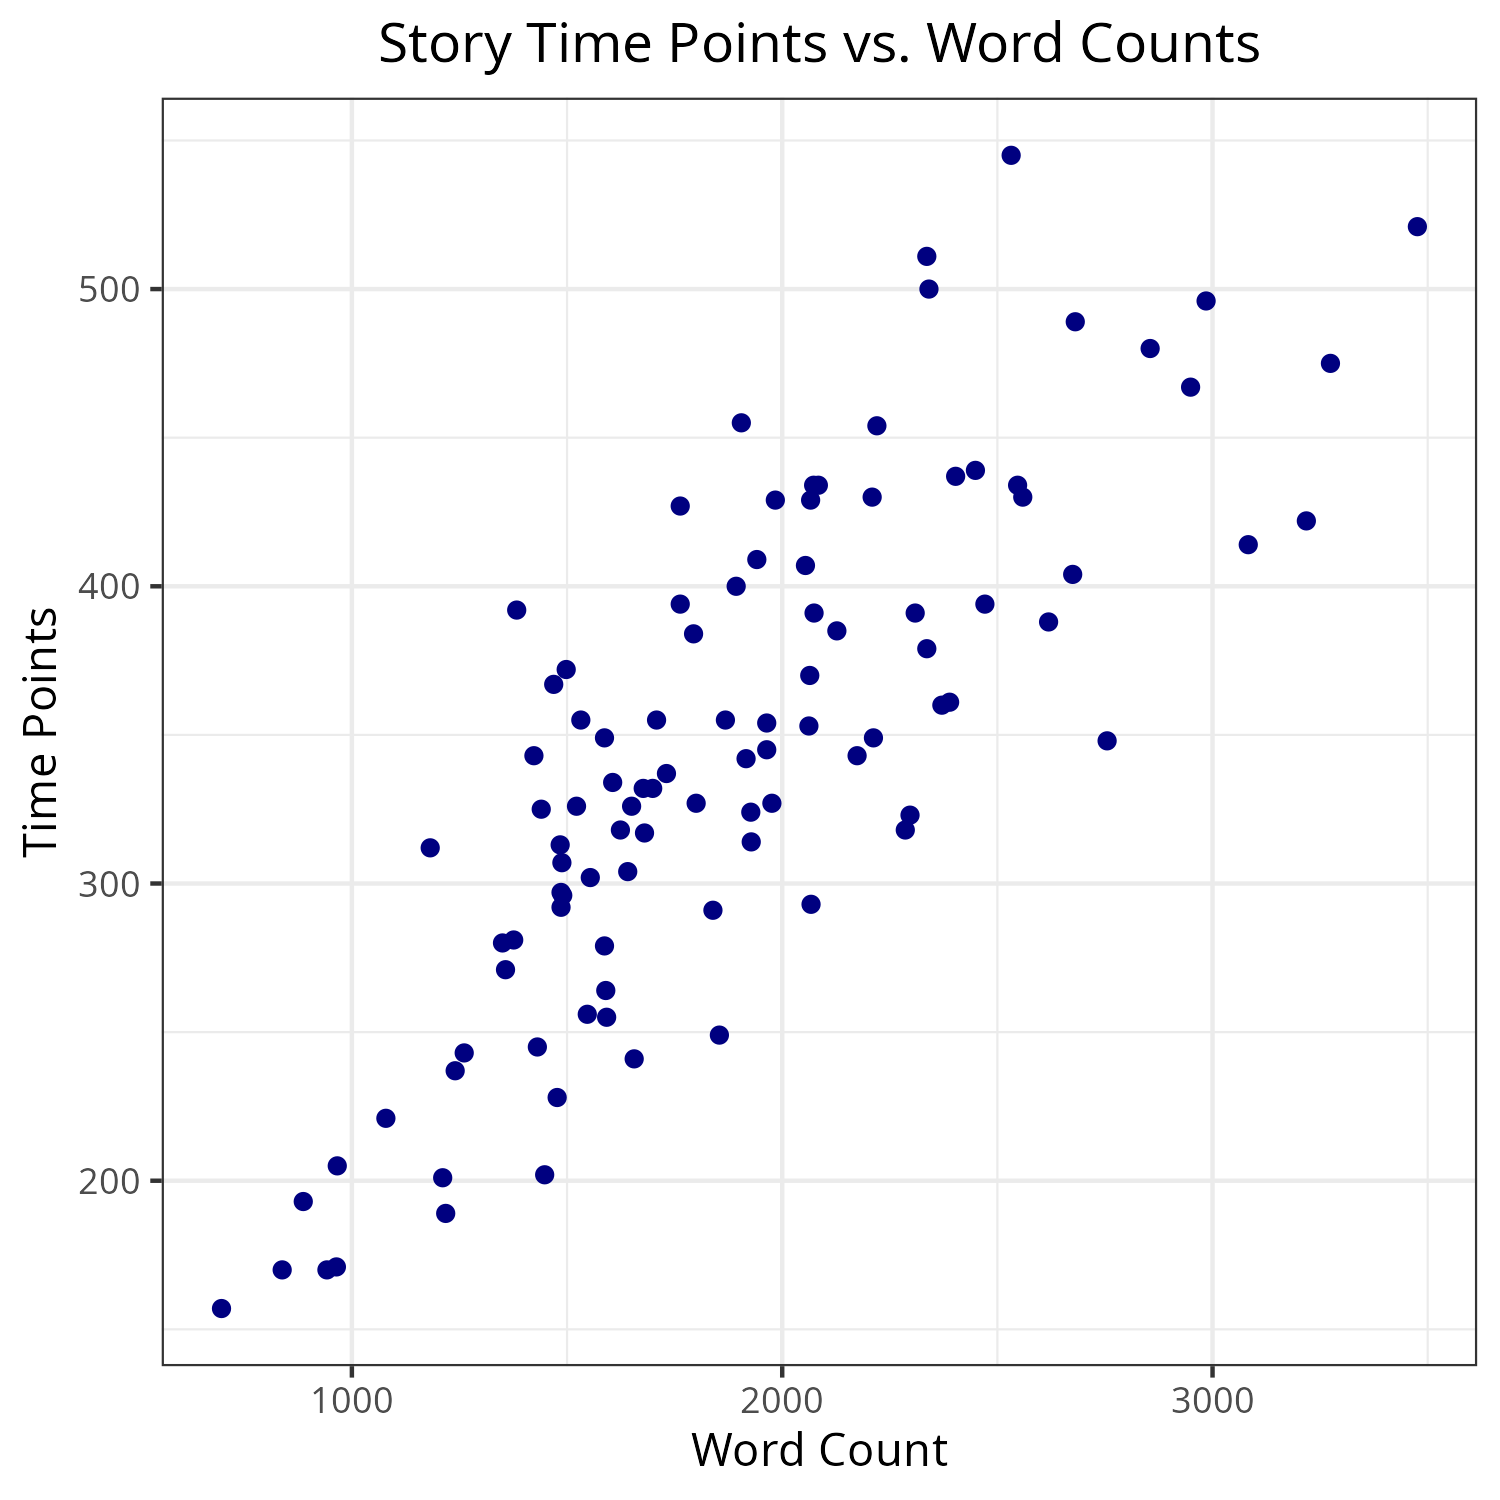
\includegraphics[width=0.6\textwidth]{figs/word_count.png}
    \caption{The number of words in a story is strongly correlated with the number of fMRI repetition time points.}
    \label{fig:word_count}
\end{figure}

To understand the basic characteristics of the BOLD signal, we analyzed the distribution of raw signal values across all voxels and time points in the training/validation set. Because plotting every individual reading is impractical, we randomly sampled 10,000 raw signal values from the training data for each subject. Figure~\ref{fig:fmri_signal} shows histograms of these sampled values for Subject 2 and Subject 3. The distributions are highly similar: both are unimodal, approximately Gaussian in shape, and centered near zero. The spread (or variance) of the raw signals also appears comparable across subjects.


\begin{figure}[ht]
    \centering
    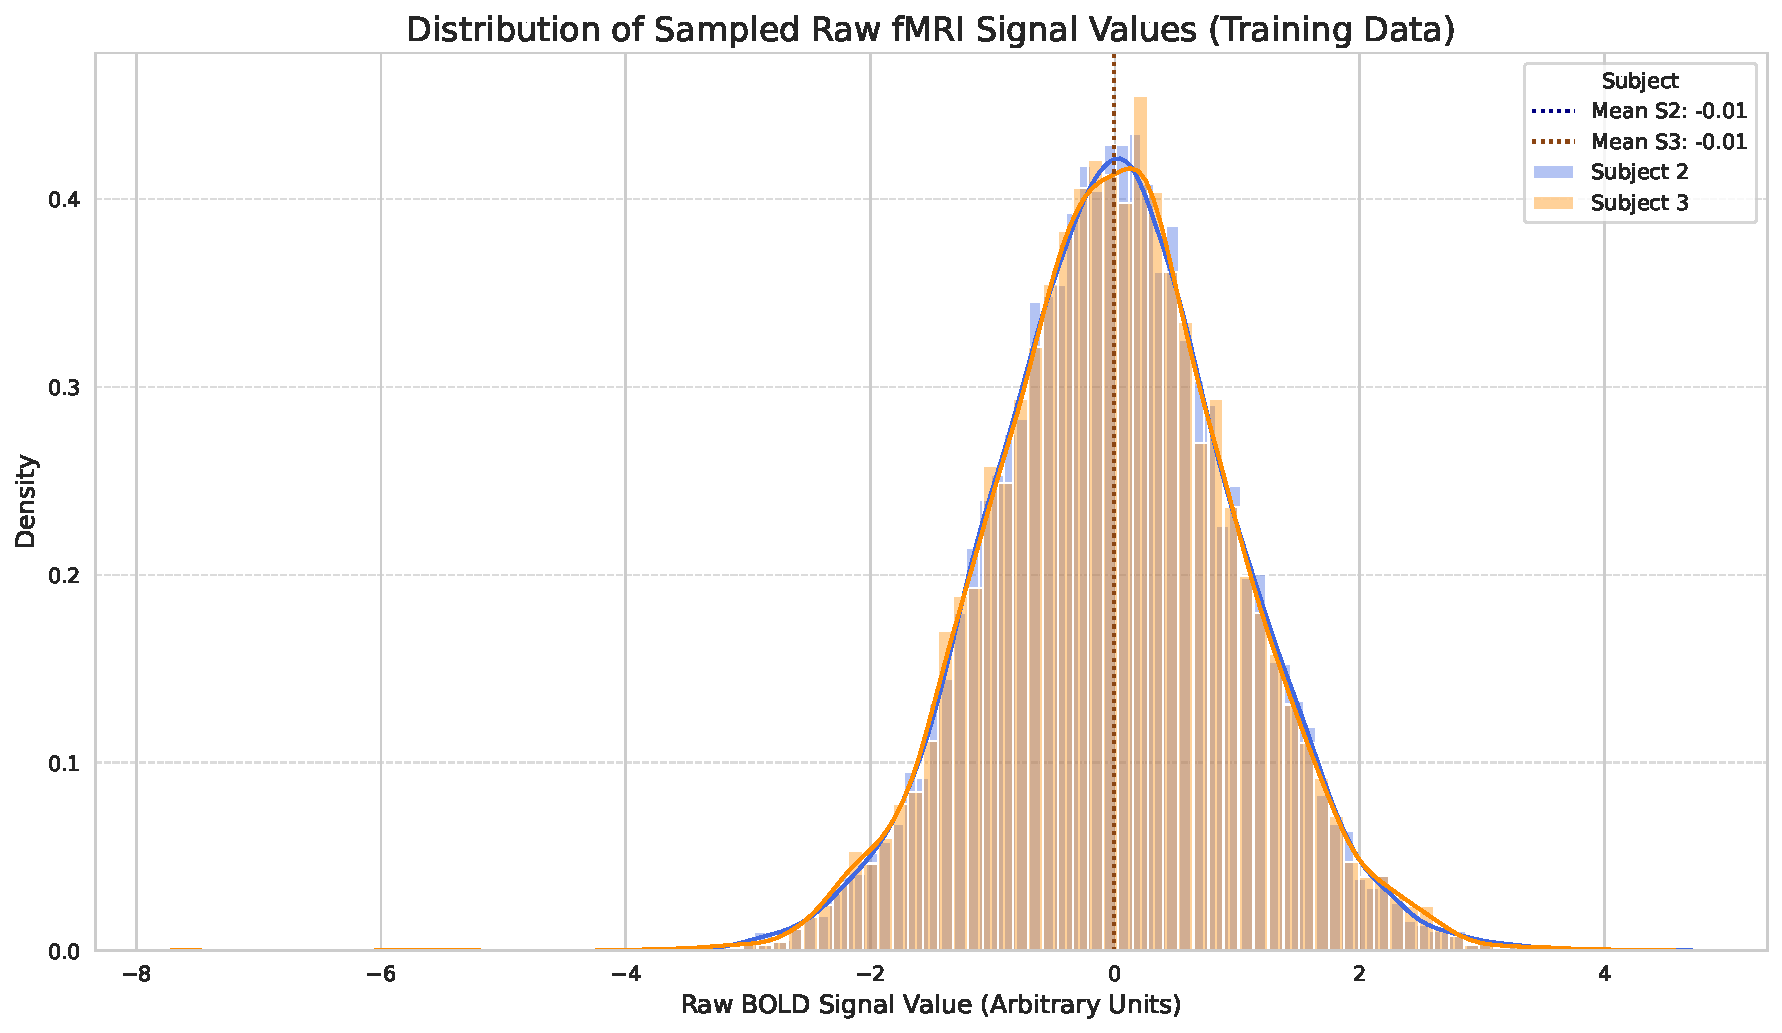
\includegraphics[width=0.8\textwidth]{figs/fmri_signal_distribution.pdf}
    \caption{Distribution of fMRI signals in training/validation dataset.}
    \label{fig:fmri_signal}
\end{figure}

In addition to examining the average fMRI signal across the entire dataset, it is informative to visualize the distribution of signals for each story individually. Figure \ref{fig:boxplots} presents the distribution of several summary statistics (mean, median, interquartile range (IQR), minimum, and maximum) computed from the fMRI signal for each of the 101 stories, where each story is treated as a single data point. The central tendency and spread (IQR) appear highly consistent across stories, while the minimum and maximum values show much greater variability. This variation in extremes may reflect story-specific events or transient noise artifacts.

\begin{figure}[ht]
    \centering
    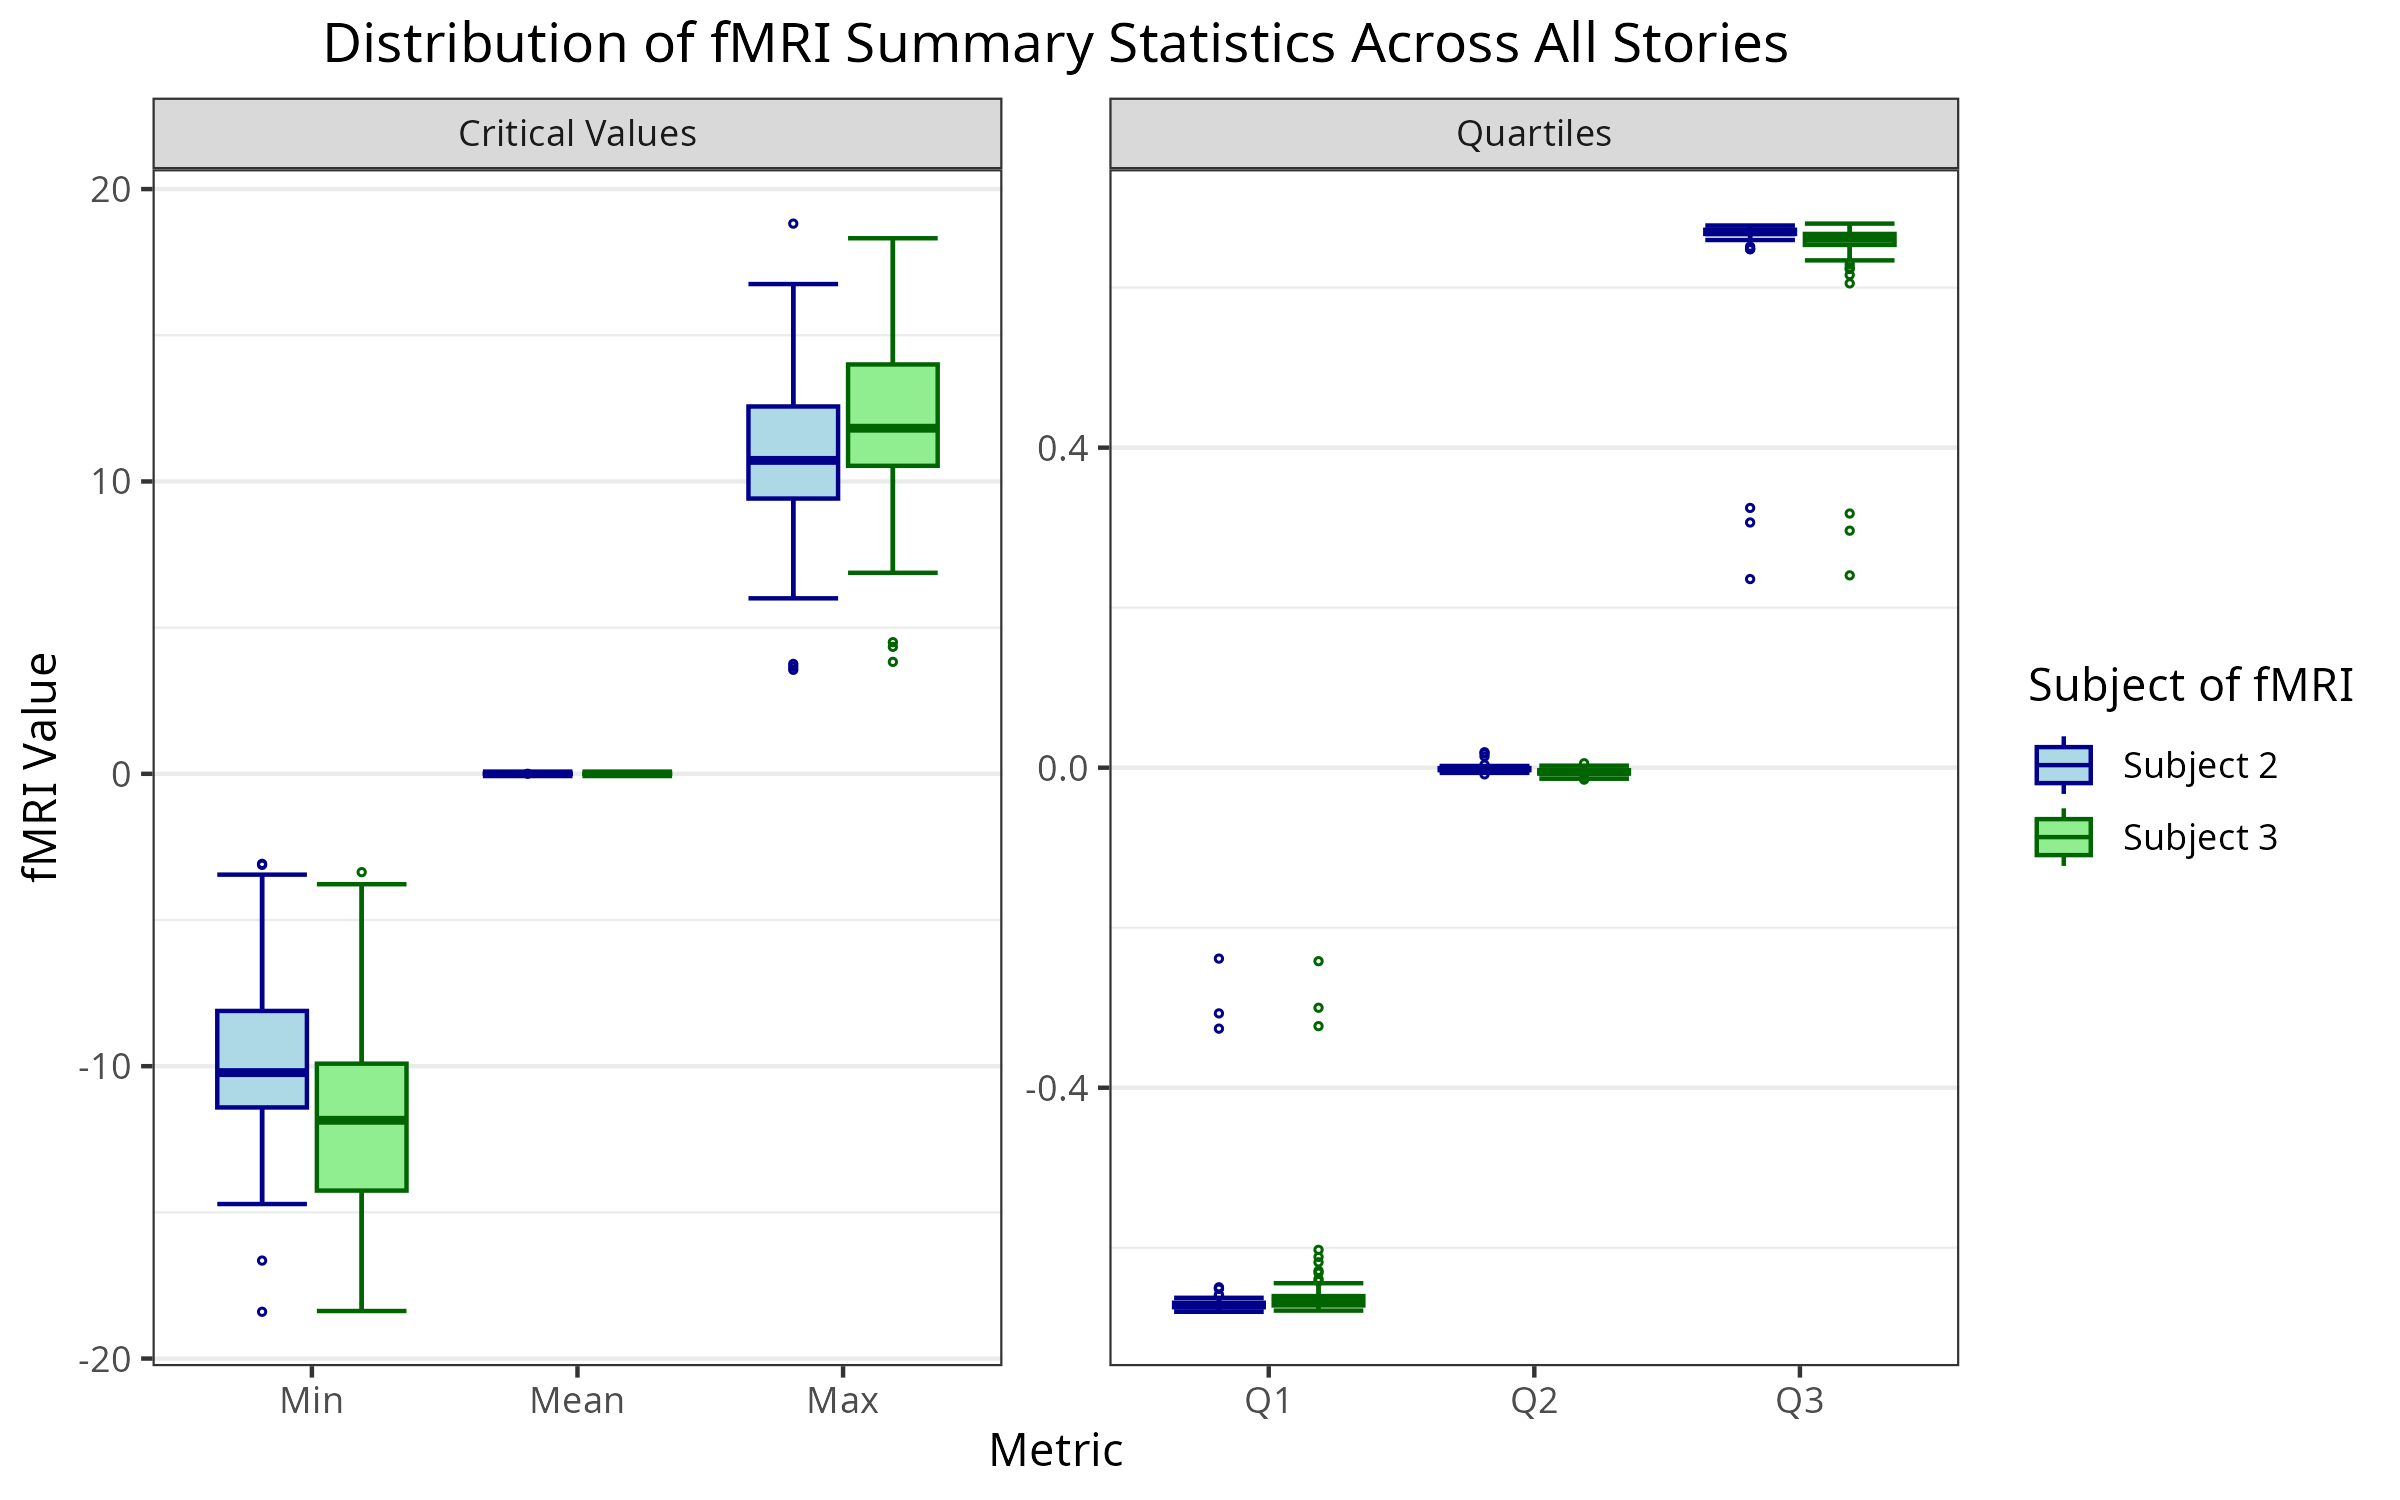
\includegraphics[width=0.8\textwidth]{figs/boxplots.png}
    \caption{Across all 101 stories, the mean, median, and interquartile range (Q1–Q3) of fMRI signals are tightly distributed, while the minima and maxima show wide variation.}
    \label{fig:boxplots}
\end{figure}

Figure \ref{fig:mean_signal} offers a more granular view by plotting the mean and IQR of the fMRI signal across all voxels at each time point within selected example stories. This enables a direct comparison of the temporal signal profiles between Subject 2 and Subject 3 over the course of each story. Despite some fluctuations, the mean signal values for both subjects consistently oscillate within a relatively narrow range (approximately –1 to 1), not only in the stories shown here but across the full set.

\begin{figure}[ht]
    \centering
    \parbox{\textwidth}{\centering 
        \fontsize{13pt}{13pt}\selectfont \textbf{Average fMRI Signal Across Selected Stories}
        
        {\fontsize{11pt}{13pt}\selectfont Mean (line) and IQR (shaded) comparison between   \textcolor{RoyalBlue}{\textbf{Subject 2}} and \textcolor{ForestGreen}{\textbf{Subject 3}}.} 
    }
    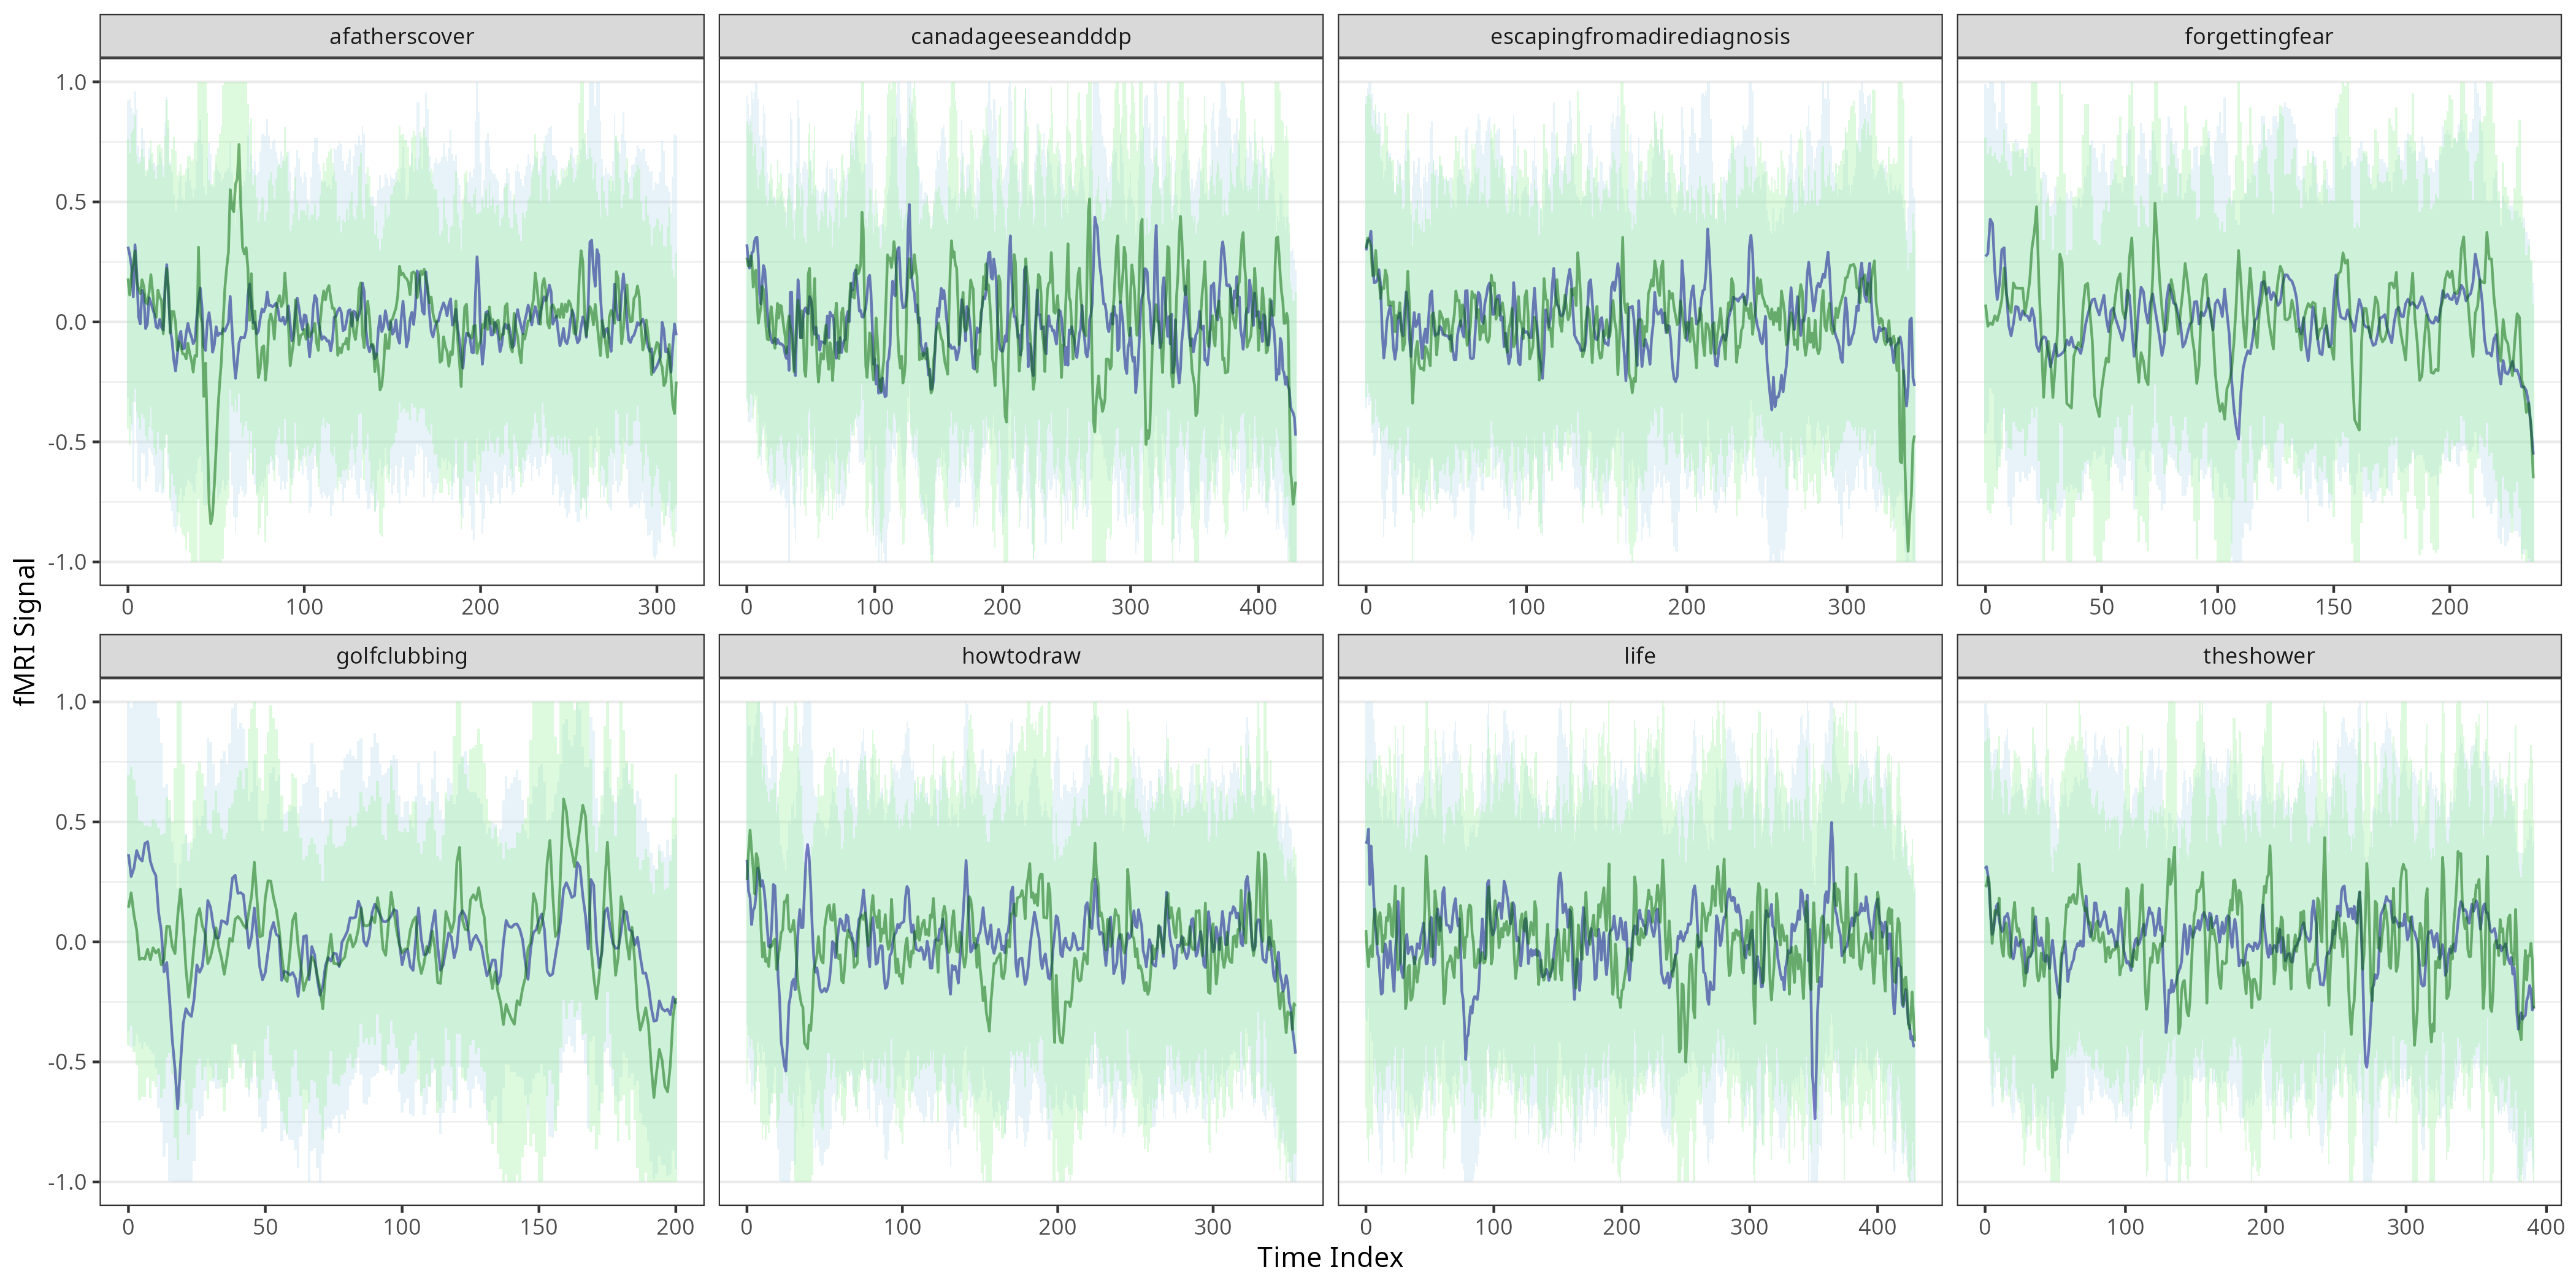
\includegraphics[width=\textwidth]{figs/mean_signal.png}
    \caption{Mean fMRI signal (line) and interquartile range (shaded area) for Subject 2 and Subject 3 at each time point, plotted separately for each story. Mean values for both subjects generally oscillate between –1 and 1.}
    \label{fig:mean_signal}
\end{figure}

In stark contrast, the maximum signal value at each time point, shown in Figure~\ref{fig:max_signal}, reveals substantial variability in peak activity levels over the course of a single story. Although some of this variation may be driven by noise, there appears to be a moderate degree of correlation or shared structure in the timing of peak signal fluctuations between the two subjects listening to the same story.

\begin{figure}[ht]
    \centering
    \parbox{\textwidth}{\centering 
        \fontsize{13pt}{13pt}\selectfont \textbf{Maximum fMRI Signal Across Selected Stories}  

        {\fontsize{11pt}{13pt}\selectfont Comparison between \textcolor{RoyalBlue}{\textbf{Subject 2}} and \textcolor{ForestGreen}{\textbf{Subject 3}}.} 
    }
    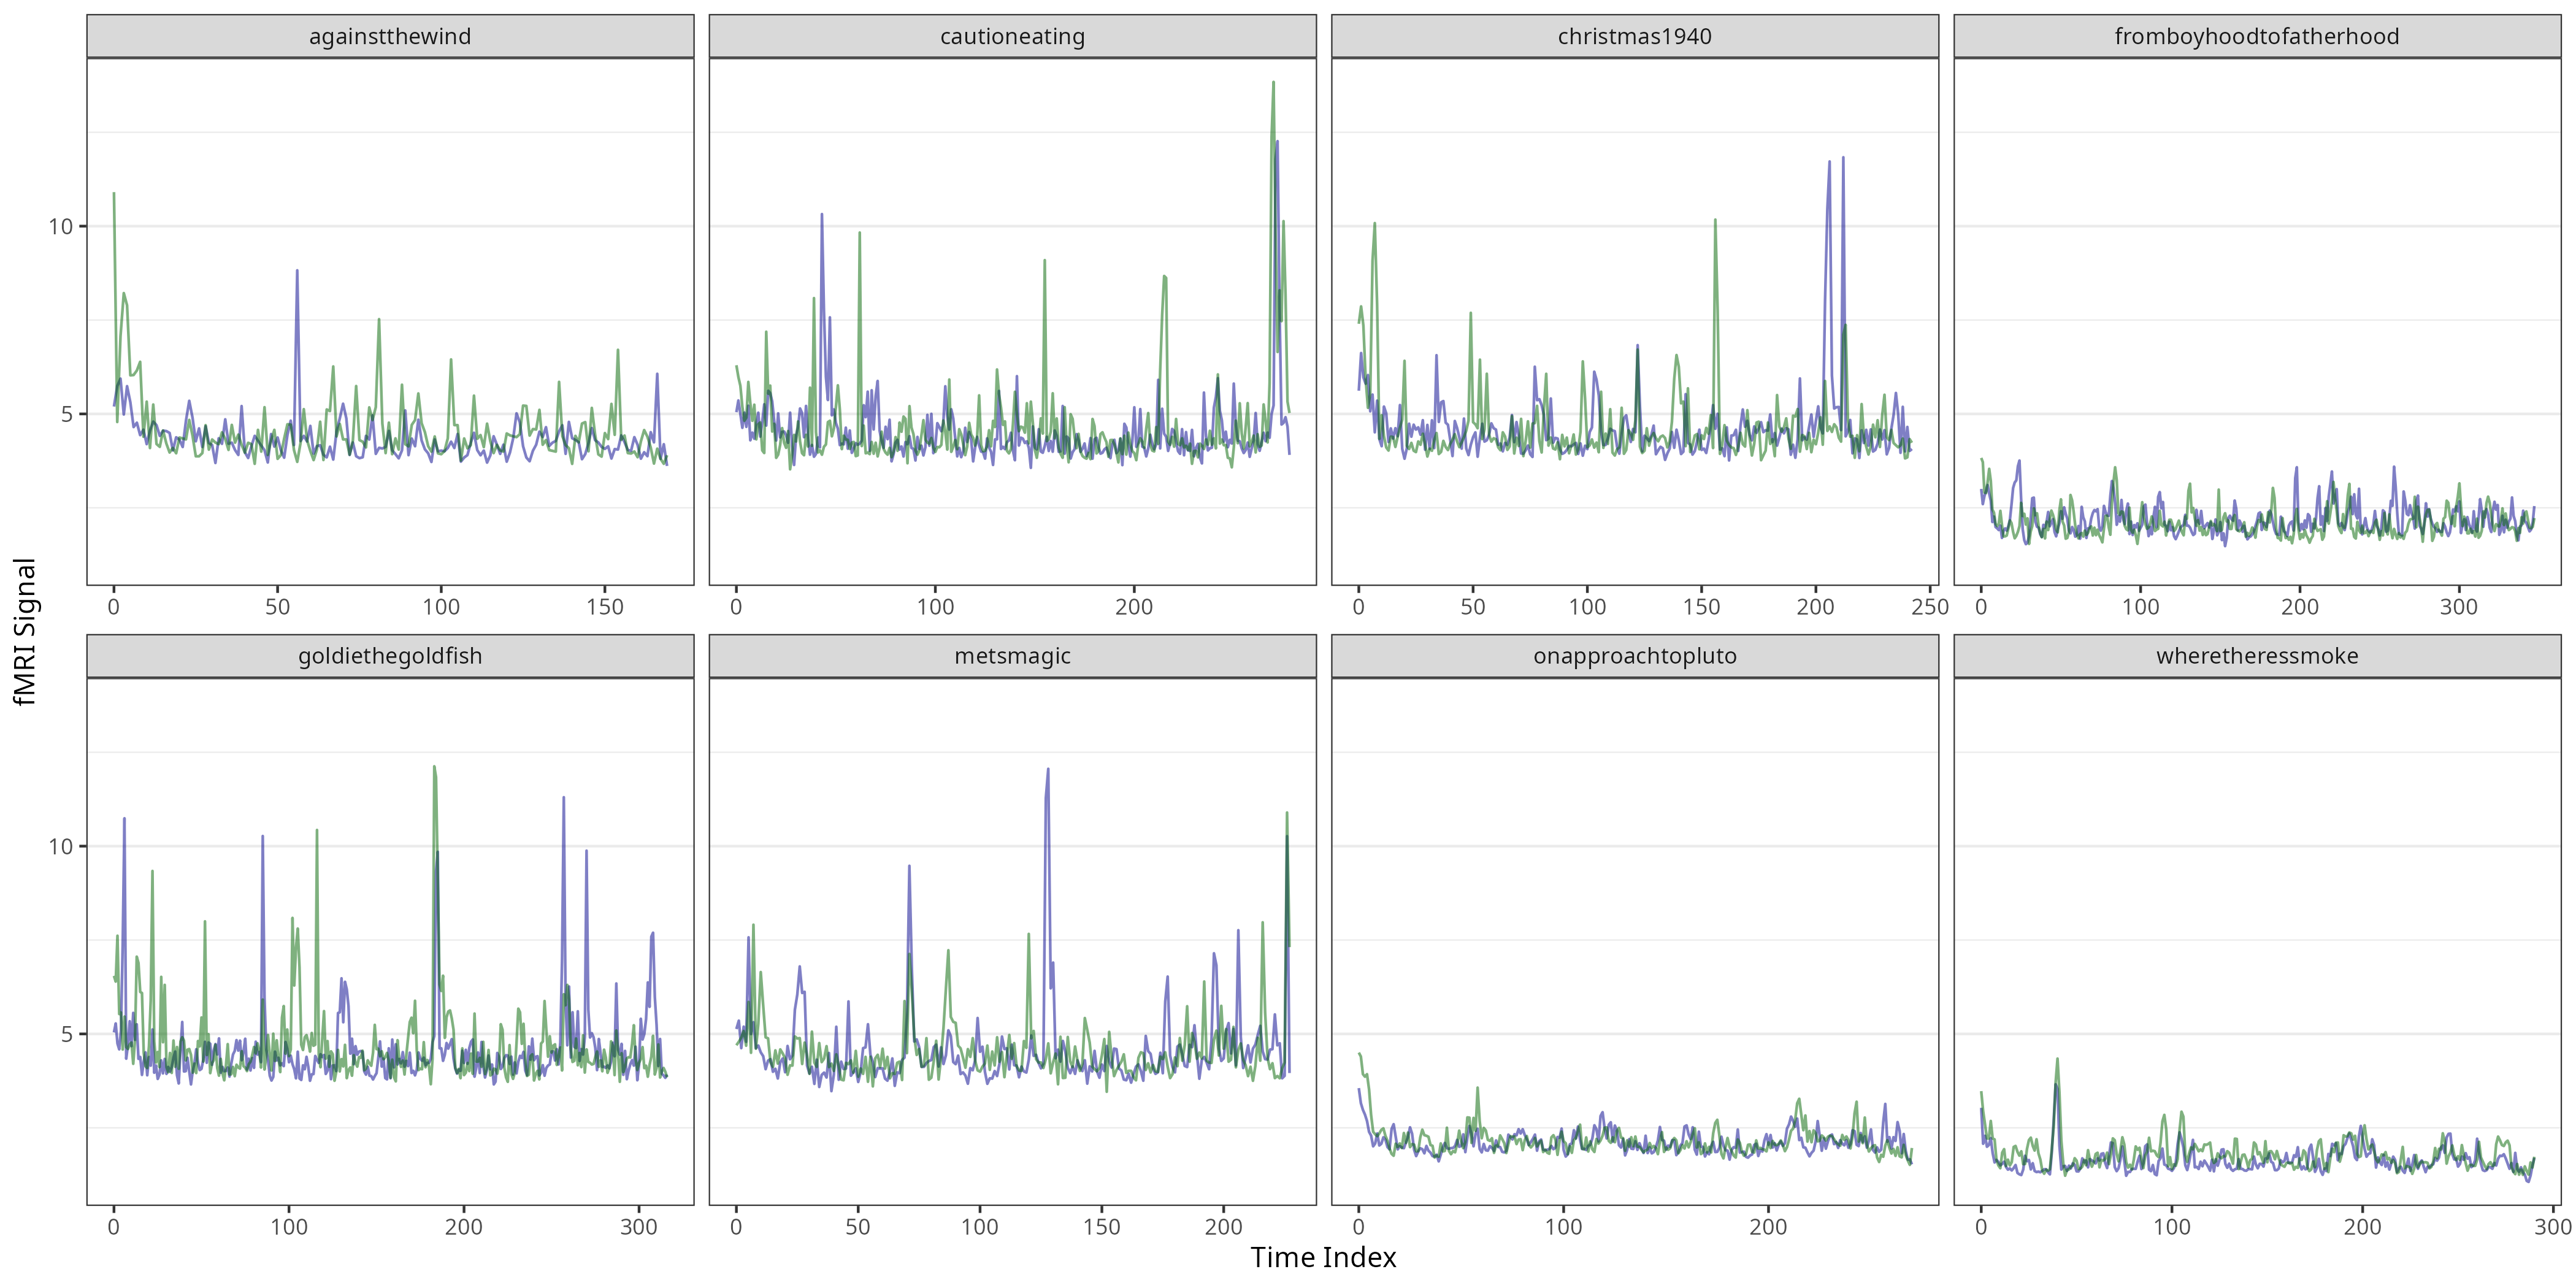
\includegraphics[width=\textwidth]{figs/max_signal.png}
    \caption{Maximum fMRI signals for Subject 2 and Subject 3 are highly correlated across several stories, despite substantial noise.}
    \label{fig:max_signal}
\end{figure}

Another thing to note is that the fMRI signals of Subject 2 contain some NaN values, which are not present in Subject 3. However, the proportion of NaN values is very small, only \(5.9 \times 10^{-6}\) of the total number of values. Due to the small proportion, we simply imputed them with the global mean to prepare the prediction and expect no significant impact on the model performance no matter which imputation method we use.


\section{Embeddings}

The primary objective of this stage is to transform the raw textual narratives from the podcast stories into numerical feature vectors aligned with the temporal resolution of the fMRI data (i.e., one feature vector per Repetition Time, TR). This process largely mirrors the methodology employed in Lab 3.2, involving the extraction of word-level embeddings and subsequent temporal aggregation. However, a key distinction in this lab is the use of the pre-trained BERT model \cite{devlin2019bert} as the source of token representations. The model can be the original BERT model or a fine-tuned version, which will be described in the following sections.

The overall pipeline for generating TR-level features is as follows:
\begin{enumerate}
    \item \textbf{Tokenization:} Each story's text is tokenized using the pre-trained tokenizer associated with BERT. This tokenizer segments words into subword units.
    \item \textbf{Token Embedding Extraction with Sliding Window:} The pre-trained BERT has a maximum input sequence length of 512 tokens. Since the stories are often longer than this limit, a sliding window approach is implemented to process the entire token sequence of each story and obtain token-level embeddings (final hidden states) from the BERT model. This process is detailed in Section \ref{ssec:sliding_window}.
    \item \textbf{Word-Level Aggregation:} For words represented by multiple subword tokens, their respective token embeddings (obtained from the sliding window output) are averaged to produce a single vector representation for each word. For words represented by a single token, their token embedding is used directly.
    \item \textbf{TR-Level Aggregation with Lanczos Resampling:} The sequence of word embeddings, timed according to their occurrence in the story, is then resampled to match the fMRI TR timings. This is achieved using Lanczos interpolation, identical to the method in Lab 3.2, which computes a weighted average of word embeddings temporally proximal to each TR.
\end{enumerate}

The resulting TR-level feature vectors serve as the input for the ridge regression models predicting fMRI voxel activity. The use of a pre-trained BERT model provides rich, context-aware initial embeddings, while the sliding window mechanism allows us to leverage this model for sequences exceeding its native context length.

\subsection{Sliding Window for Token Embedding Extraction}
\label{ssec:sliding_window}

The BERT model is restricted to processing input sequences of at most 512 tokens. To derive token embeddings for entire stories, which typically exceed this length, we implement a sliding window technique. This technique processes the full token sequence of a story in manageable, overlapping segments.

The procedure is as follows:
\begin{enumerate}
    \item \textbf{Chunking:} The complete sequence of input token IDs for a story is divided into chunks of a fixed window size (set to 512 tokens, matching the BERT model's limit).
    \item \textbf{Striding and Overlap:} These chunks are extracted with a specified stride (set to 256 tokens). A stride smaller than the window size ensures that consecutive windows overlap. This overlap is beneficial as tokens appearing near the boundaries of one chunk will also appear in more central, and thus potentially better contextualized, positions in adjacent chunks.
    \item \textbf{BERT Processing:} Each chunk of tokens, along with its corresponding attention mask segment, is passed independently through the pre-trained BERT. The model outputs the final hidden states (embeddings) for every token within that chunk.
    \item \textbf{Aggregation of Token Embeddings:} Since a single token from the original long sequence might appear in multiple overlapping windows, its representation is computed by averaging the hidden states obtained for that token from all the chunks in which it was processed. This is achieved by summing the embedding vectors for each token position across all chunks covering it and then dividing by the number of times that position was included in a chunk.
\end{enumerate}
The result of this sliding window process is a sequence of token embeddings with the same length as the original tokenized story, where each token embedding \( \mathbf{e}_i \in \mathbb{R}^{768} \) has been informed by a local context of up to 512 tokens. These aggregated token embeddings are then used for the word-level aggregation, and finally for the TR-level aggregation.

\subsection{Differentiability of the Embedding Process}
The embedding process described above is fully differentiable, meaning that the gradients can be backpropagated through the entire pipeline. This allows for the possibility of fine-tuning the BERT, enabling it to adapt to the fMRI data and the language processing tasks at hand. By allowing gradients to flow through the token embedding, sliding window, and aggregation steps, we can optimize the entire embedding process jointly with pretrained BERT.

\section{Modeling - Pre-Trained Embeddings}

\subsection{Modeling Approach}
We create a predictive model to predict fMRI levels for each voxel using the pre-trained embeddings we have generated. Specifically, we fit a ridge regression model. This modeling approach contains the parameter alpha, which controls the penalty term on the model's weights as L2 (squared) loss.

We start by fitting a regression model for Subject 2, for each different embedding - Bag of Words, GloVe, and Word2Vec. Using the cross-validation strategy described in the next section, we find the best alpha hyperparameter value for regularization.

\subsection{Model Evaluation Strategy}

We utilize a standard k-fold cross-validation strategy to develop our predictive models. The split is done at a story level instead of a TR level to mimic the real-world scenario where the model is trained on a set of stories and then evaluated on unseen stories. 60\% of the stories are used for training and validation, and the remaining are reserved for testing and remain untouched until the final evaluation.

For each fold, the bag-of-words is retrained on the training data to avoid data leakage, while the pre-trained embeddings are applied before the data split as they are fixed and independent of the training data.

The metric we use to evaluate the model performance is the correlation coefficient (CC) between the predicted and actual fMRI signals, which is a standard metric in the context of fMRI signals. We do this per voxel, giving us a voxel-wise CC. This is the metric that our model is trained to optimize for.

This strategy is designed to mimic the real-world scenario with the best efforts to avoid data leakage and measure the model's generalization performance.

\subsection{Results}

Our cross-validation results for hyperparameter tuning are shown in Tables \ref{tab:word2vec_cv}, \ref{tab:glove_cv}, and \ref{tab:bow_cv} for the models trained with the Word2Vec, GloVe, and Bag of Words embeddings, respectively. These are performance metrics on the validation set.


\begin{table}[ht]
\centering
\caption{Performance metrics for Word2Vec at different values of \texttt{alpha}. Best alpha: 1000 (Mean CV CC = 0.0057).}
\label{tab:word2vec_cv}
\begin{tabular}{rrrrr}
\toprule
\textbf{Alpha} & \textbf{Mean CC} & \textbf{Median CC} & \textbf{Top1 CC} & \textbf{Top5 CC} \\
\midrule
0.1    & 0.0035 & 0.0032 & 0.0462 & 0.0325 \\
1      & 0.0036 & 0.0032 & 0.0462 & 0.0325 \\
10     & 0.0036 & 0.0032 & 0.0463 & 0.0325 \\
100    & 0.0039 & 0.0035 & 0.0478 & 0.0330 \\
1000   & 0.0057 & 0.0051 & 0.0518 & 0.0364 \\
\bottomrule
\end{tabular}
\end{table}

\begin{table}[ht]
\centering
\caption{Performance metrics for GloVe at different values of \texttt{alpha}. Best alpha: 1000 (Mean CV CC = 0.0067).}
\label{tab:glove_cv}
\begin{tabular}{rrrrr}
\toprule
\textbf{Alpha} & \textbf{Mean CC} & \textbf{Median CC} & \textbf{Top1 CC} & \textbf{Top5 CC} \\
\midrule
0.1    & 0.0048 & 0.0044 & 0.0474 & 0.0337 \\
1      & 0.0048 & 0.0044 & 0.0474 & 0.0337 \\
10     & 0.0058 & 0.0046 & 0.0479 & 0.0341 \\
100    & 0.0055 & 0.0051 & 0.0496 & 0.0352 \\
1000   & 0.0067 & 0.0061 & 0.0535 & 0.0377 \\
\bottomrule
\end{tabular}
\end{table}

\begin{table}[ht]
\centering
\caption{Performance metrics for BoW at different values of \texttt{alpha}. Best alpha: 1000 (Mean CV CC = 0.0230).}
\label{tab:bow_cv}
\begin{tabular}{rrrrr}
\toprule
\textbf{Alpha} & \textbf{Mean CC} & \textbf{Median CC} & \textbf{Top1 CC} & \textbf{Top5 CC} \\
\midrule
0.1    & 0.0063 & 0.0062 & 0.0451 & 0.0338 \\
1      & 0.0084 & 0.0082 & 0.0486 & 0.0368 \\
10     & 0.0098 & 0.0095 & 0.0514 & 0.0392 \\
100    & 0.0141 & 0.0135 & 0.0614 & 0.0476 \\
1000   & 0.0230 & 0.0213 & 0.0851 & 0.0676 \\
\bottomrule
\end{tabular}
\end{table}




From this cross-validation process, the best model ended up being the Bag of Words model which used an alpha of 1000. It had a mean test CC of 0.0009, median CC of 0.0009, Top 1 percentile CC of 0.0311, and Top 5 Percentile CC of 0.0215. Overall, the CC is low (our model has a limited ability to predict fMRI levels well), and slightly higher than a random guessing.



\subsection{Detailed Evaluation \& Analysis}
For the model with the best embedding, which was Bag of Words, we performed a more detailed evaluation. We examine the distribution of test CC across voxels. We generate a list of CCs (one for each voxel), then visualize see how the CC is distributed across voxels. We are looking to see how differently the model performs on some voxels in comparison with others if they all have similar performance, or if there is a skew/outlier voxels, etc. Figure \ref{fig:cc_dist_voxels_subject_2} describes the distribution of CC across voxels. We can see that the distribution is relatively symmetric, with no major skew. Numerically, the distribution of CC is centered around 0.0009, with a 25th percentile above -0.01 and a 75th percentile at approximately 0.01. An important note is that there are numerous outlier voxels on either side (based on the 1.5*IQR outlier threshold), which suggests that the spread of CC across voxels is relatively large. The positive outliers are stronger/slightly further from the center than the negative outliers.

So, this model does not perform the same across all voxels. Scientifically, this implies that prediction in different voxels of the brain has varying levels of difficulty. This could stem from that some brain areas (voxels) are irreverent from language processing, or at least language processing in listening to these stories, leading to noise that cannot be predicted with the story text, while some others actively respond to the story. However, more domain knowledge is required to justify the hypothesis.

We want to have a reasonable interpretation criterion for interpreting voxels according to PCS. We want to make sure that the predictions are meaningfully better than by chance. One option is to only select voxels in the top \(x\) percentile of the observed distribution of CCs (i.e. for \(x=5\) for the 5th percentile). The reason to select the top voxels is that we know they respond to the stories actively, while others could be just random noise, as stated before. In terms of stability, we would ideally want to be able to predict voxels well across different stories, subjects, etc. We could check this by examining each voxel's CC across model performance for different stories, or different models for different subjects. Lastly, we want the full prediction process to be reproducible and computed reliably. These conditions align with the three main parts of PCS.


\begin{figure}
    \centering
    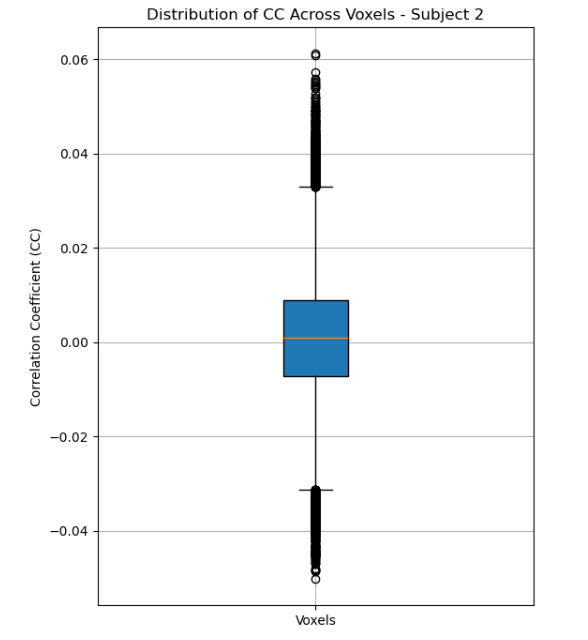
\includegraphics[width=0.5\linewidth]{figs/cc_dist_voxels_subject_2.png}
    \caption{Distribution of CC across voxels for Subject 2 using Bag of Words embeddings.}
    \label{fig:cc_dist_voxels_subject_2}
\end{figure}


\subsection{Stability Analysis}
We conduct a stability analysis by examining performance across different subjects. In this case, we compare Subject 2, which has been detailed so far, with another model trained on Subject 3. We train and test a model on Subject 3 using the same stories as Subject 2. We can then compare the distributions of CCs to see how stable the process is across different subjects.

Our final Subject 3 model uses the Bag of Words embedding and an alpha hyperparameter of 1000 for Ridge. After the training, the final test set performance for Subject 3 was a mean CC of 0.0017, median CC of 0.0014, top 1 percentile CC of 0.0320, and a top 5 percentile CC of 0.0213. This is shown in Table \ref{tab:subject_performance}. In comparison with Subject 2, we note that the top 1 percentile and top 5 percentile CCs are very similar, which suggests stable results. The mean and median CC are better for Subject 3, though not by a large margin that would suggest high instability.

\begin{table}[ht]
  \centering
  \caption{Test Performance Metrics for Subject 2 and Subject 3}
  \label{tab:subject_performance}
  \begin{tabular}{lcccc}
    \hline
    \textbf{Subject} & \textbf{Mean Test CC} & \textbf{Median Test CC} & \textbf{Top 1 Percentile CC} & \textbf{Top 5 Percentile CC} \\
    \hline
    Subject 2        & 0.0009                & 0.0009                 & 0.0311                     & 0.0215                      \\
    Subject 3        & 0.0017                & 0.0014                 & 0.0320                     & 0.0213                      \\
    \hline
  \end{tabular}
\end{table}

We also visualize the distribution of CC across voxels to have a deeper understanding and comparison with Subject 2. This is shown in Figure \ref{fig:cc_dist_voxels_subject_3}. Visually, the distributions of CC across voxels look very similar between Subject 2 and Subject 3. The medians and quartiles, and outliers also show no major differences. This suggests a generally stable result.

\begin{figure}
    \centering
    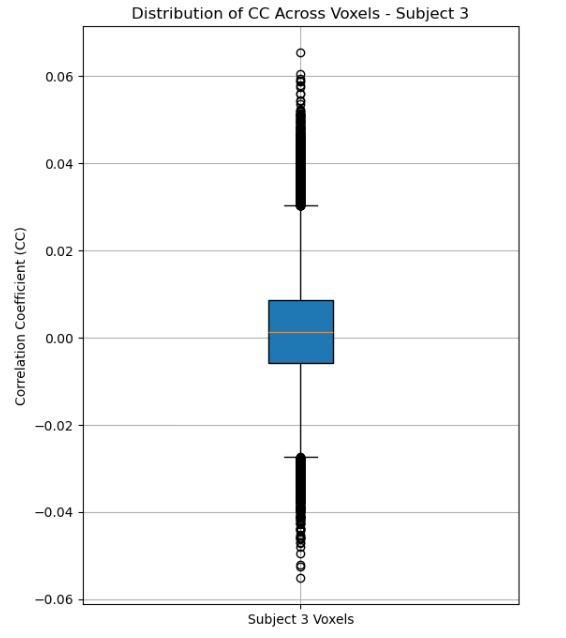
\includegraphics[width=0.5\linewidth]{figs/cc_dist_voxels_subject_3.png}
    \caption{Distribution of CC across voxels for Subject 3 using Bag of Words embeddings.}
    \label{fig:cc_dist_voxels_subject_3}
\end{figure}


\section{Modeling - Encoder Embedding}

In this section, we now fit a linear model using the embeddings generated from the BERT-style encoder, as opposed to the pretrained embeddings. Doing so will allow us to examine if using an encoder shows potential for better predictions than pretrained embeddings, and how they differ. We follow a similar cross validation process, testing values across the 0.1 - 1000 range for the Ridge hyperparameter alpha.

\subsection{Encoder Embedding Model - Hyperparameter Selection}
We utilized the same cross-validation strategy as in the previous section. The hyperparameter training results for selecting the alpha value are shown in Table \ref{tab:encoder_cv}. Based on the CC scores, we selected alpha=1000 as the best value.

\begin{table}[ht]
\centering
\caption{Performance metrics for encoder embeddings at different values of $\alpha$. Best alpha: 1000 (Mean CV CC = $-0.0052$).}
\label{tab:encoder_cv}
\begin{tabular}{rrrrrr}
\toprule
\textbf{Alpha} & \textbf{Mean CC} & \textbf{Median CC} & \textbf{Top1 CC} & \textbf{Top5 CC} & \textbf{Top10 CC} \\
\midrule
0.1   & -0.0055 & -0.0060 & 0.0382 & 0.0233 & \multicolumn{1}{c}{--} \\
1     & -0.0055 & -0.0060 & 0.0382 & 0.0233 & \multicolumn{1}{c}{--} \\
10    & -0.0056 & -0.0060 & 0.0382 & 0.0233 & \multicolumn{1}{c}{--} \\
100   & -0.0052 & -0.0058 & 0.0393 & 0.0240 & \multicolumn{1}{c}{--} \\
1000  & -0.0052 & -0.0058 & 0.0393 & 0.0240 & \multicolumn{1}{c}{--} \\
\bottomrule
\end{tabular}
\end{table}

\subsection{Encoder Embedding Model - Results}

On the test set, the best model for the encoder embedding (with alpha=1000) reached a mean CC of 0.0060 for Subject 2 and a mean CC of 0.0114. Interestingly, for the encoder embeddings, we see not only significantly greater performance overall but also a larger difference in magnitude between the CC of Subject 2 and Subject 3, which will be examined in further depth. These results are shown in Table \ref{tab:cc_pretrained_vs_encoder_comparison}.


\begin{figure}[ht]
    \centering
    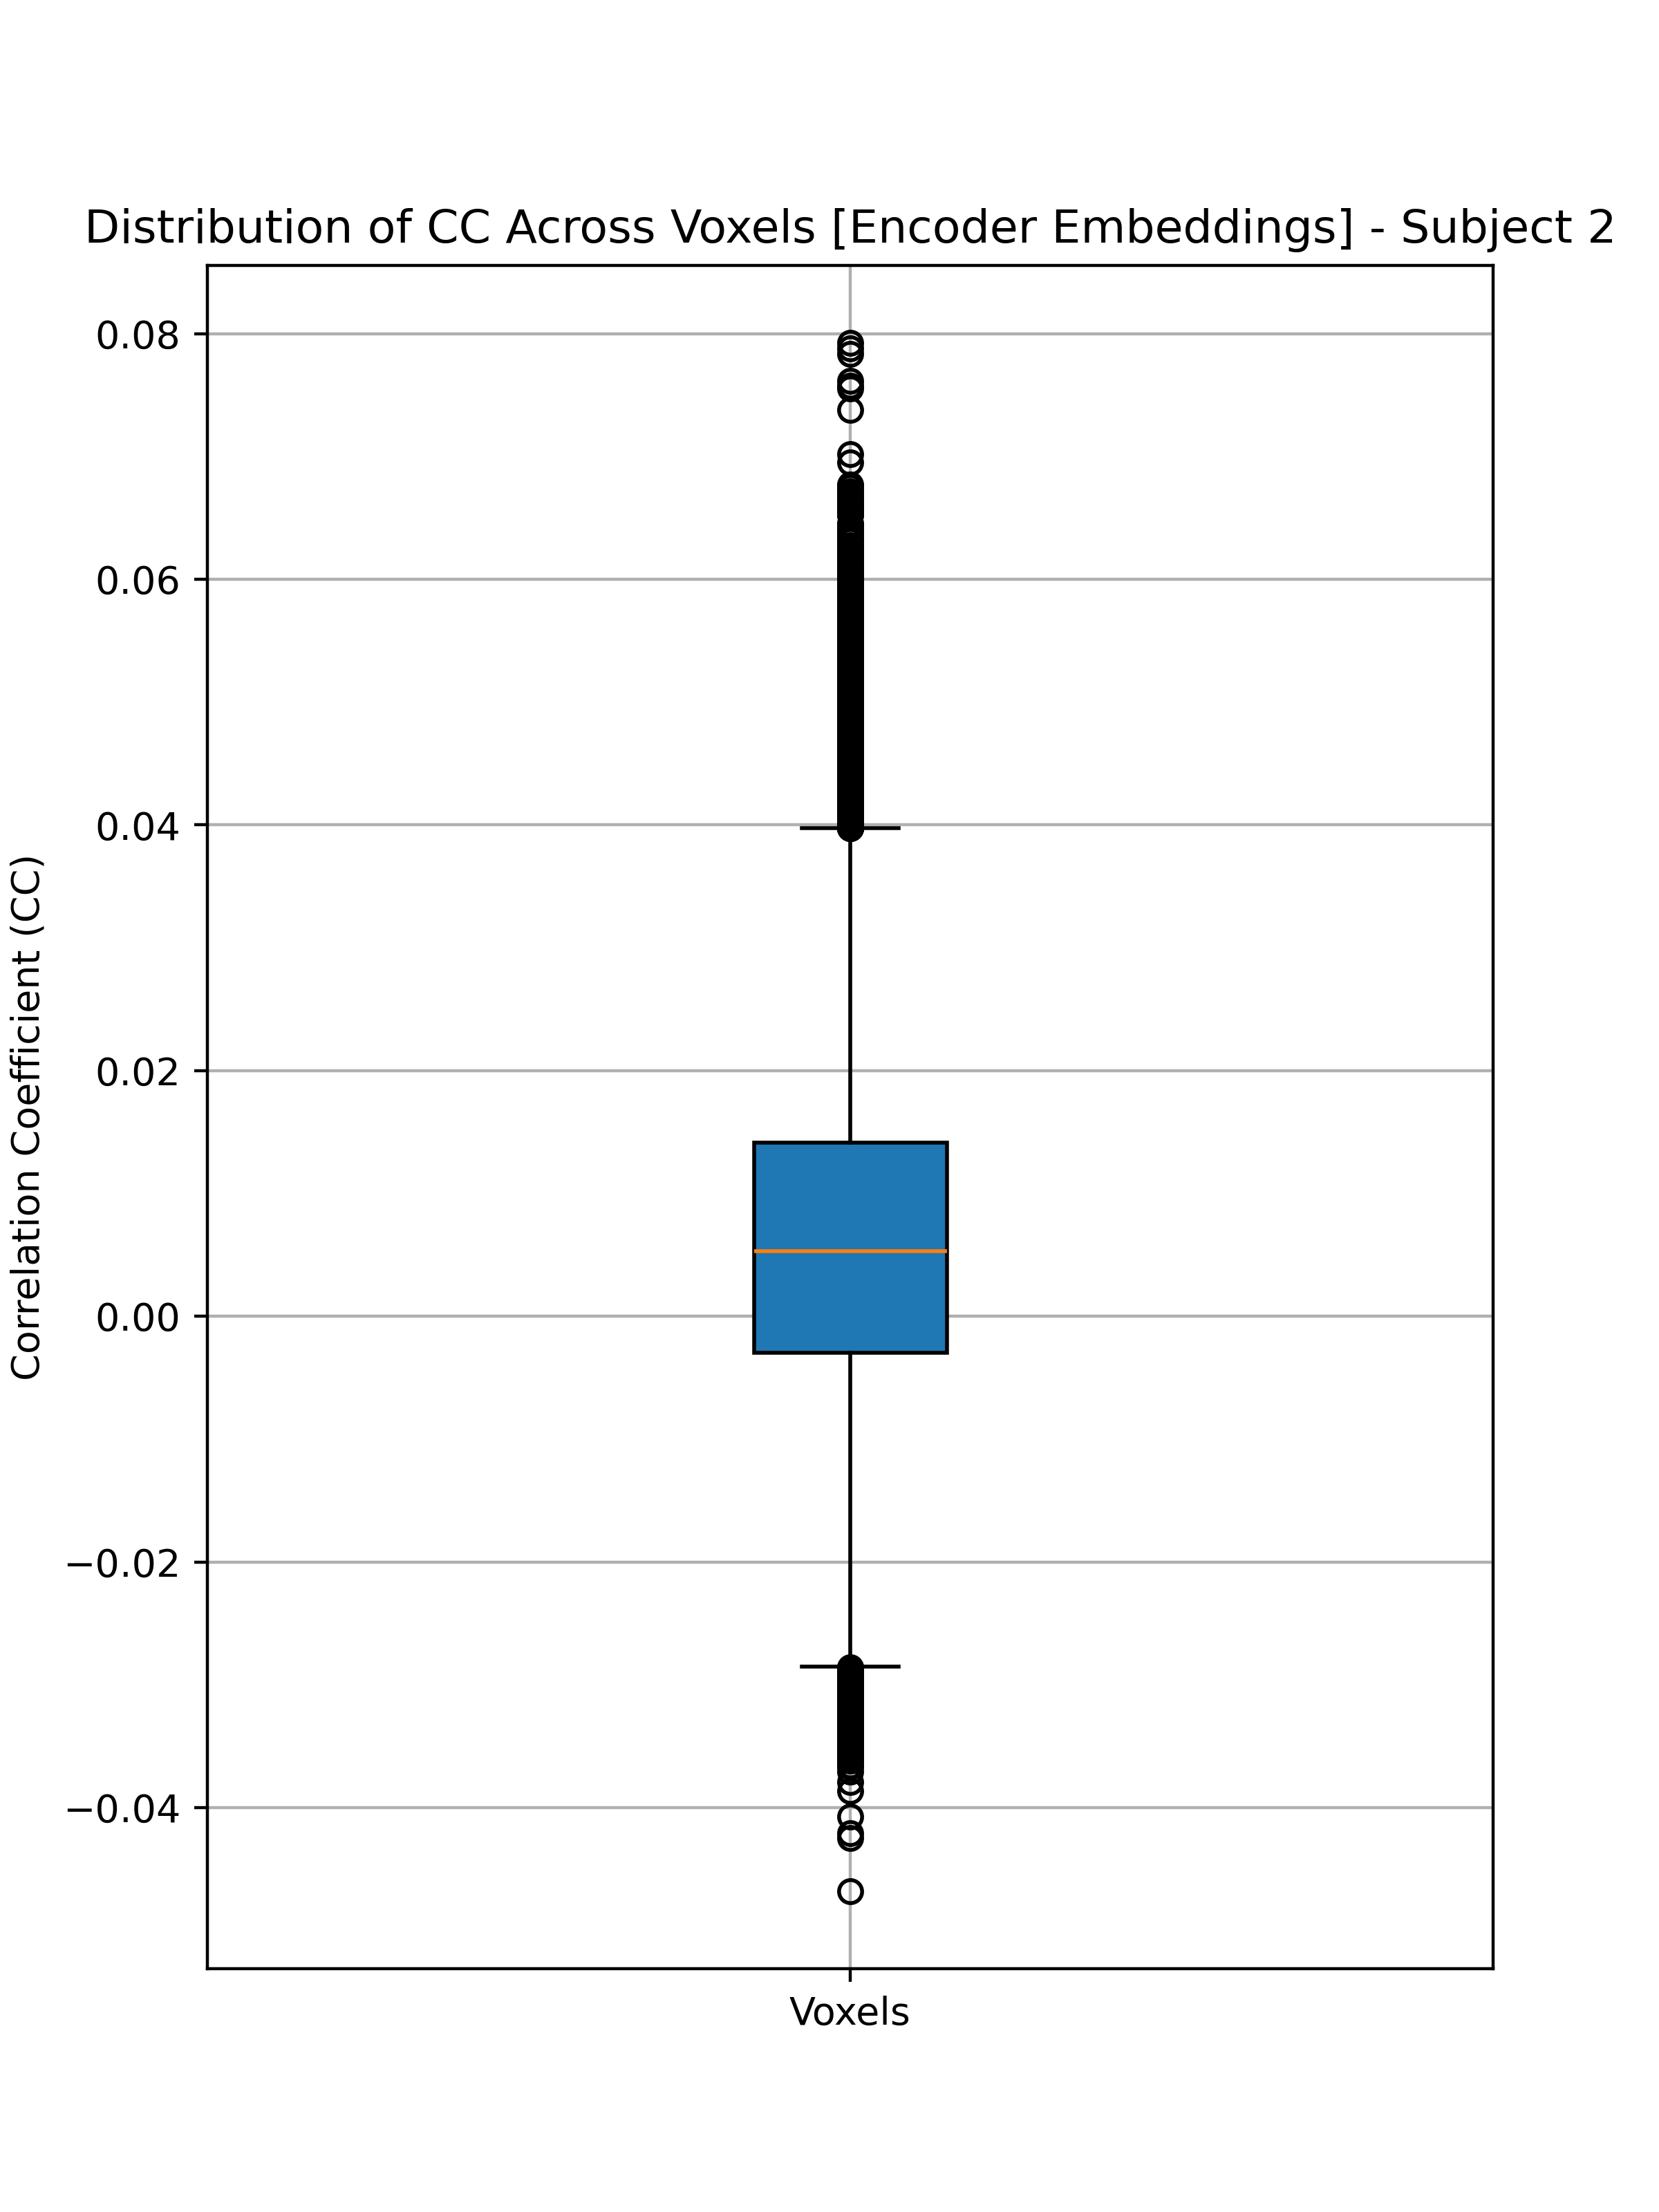
\includegraphics[width=0.5\linewidth]{figs/encoder_subj2_cc_dist.png}
    \caption{Distribution of CC across voxels for Subject 2 using Encoder embeddings.}
    \label{fig:cc_dist_encoder_subject_2}
\end{figure}

\subsection{Encoder Embedding Model - Detailed Evaluation \& Analysis}
We examine the distribution of test CC for the encoder embedding Ridge model across voxels. Figure \ref{fig:cc_dist_encoder_subject_2} describes the distribution of CC across voxels for Subject 2. We can see that the distribution is somewhat symmetric, with a slight upward skew. Numerically, the distribution of CC is centered around 0.007, with a 25th percentile around -0.01 and a 75th percentile at approximately 0.04. An important note is that there are numerous outlier voxels on either side (based on the 1.5*IQR outlier threshold), which suggests that the spread of CC across voxels is relatively large. The positive outliers are more numerous and stronger/further from the center than the negative outliers, reflecting a slight upward skew. One interesting note is that this distribution of CC is generally shifted more upward than the pre-trained embedding (i.e., Bag of Words) model, and has more positive outliers.

So, this model does not perform the same across all voxels, just as we saw with the model using pre-trained embeddings. Scientifically, this implies that prediction in different voxels of the brain has varying levels of difficulty. This could stem from that some brain areas (voxels) are irrelevant to language processing, or at least language processing in listening to these stories, leading to noise that cannot be predicted with the story text, while some others actively respond to the story. To investigate this further, more domain knowledge would be useful.

As stated earlier, we want to have a reasonable interpretation criterion for interpreting voxels according to PCS. We want to make sure that the predictions are meaningfully better than by chance. One option is to only select voxels in the top \(x\) percentile of the observed distribution of CCs (i.e., for \(x=5\) for the 5th percentile). The reason to select the top voxels is that we know they respond to the stories actively, while others could be just random noise, as stated before. In terms of stability, we would ideally want to be able to predict voxels well across different stories, subjects, etc. We could check this by examining each voxel's CC across model performance for different stories, or different models for different subjects. Lastly, we want the full prediction process to be reproducible and computed reliably. These conditions align with the three main parts of PCS.


\subsection{Pre-Trained vs. Encoder Embeddings Comparison}

We compare the results of the encoder embedding against the pre-trained embeddings by examining the CC of the encoder model and the Bag of Words model (which was the best pre-trained model). We see that the encoder embeddings are able to reach a higher CC. This is true across all thresholds of CC, including mean, median, Top 1\%, and Top 5\% CC. In particular, the top performance of voxels (for Top 1\% and Top 5\% are closer) is closer, while the mean and median CCs are much higher for the model using encoder embeddings. This can mean that the encoder embeddings generally provide better performance throughout more voxels, whereas the pre-trained embeddings only provide comparable performance at their best voxels. As mentioned, the distribution of CC is generally shifted more upward for the encoder embedding than the pre-trained embedding (i.e., Bag of Words) model, and has more positive outliers. This is shown when comparing the boxplots of the CC distribution across voxels in Figures \ref{fig:cc_dist_voxels_subject_2} and \ref{fig:cc_dist_encoder_subject_2}.

In summary, different embedding methods do not perform equally well across the voxels. The encoder embeddings tend to have better performance across more voxels, whereas the pre-trained embeddings tend to have far worse performance for most voxels. However, the pre-trained embeddings still provide comparable performance to the encoder embeddings for the top-performing voxels for both models.


\begin{table}[ht]
\centering
\caption{Comparison - Test Performance Metrics for Bag-of-Words vs. Pre-Trained Embeddings}
\label{tab:cc_pretrained_vs_encoder_comparison}
\begin{tabular}{llrrrr}
\toprule
\textbf{Embedding}   & \textbf{Subject} & \textbf{Mean CC} & \textbf{Median CC} & \textbf{Top 1 \% CC} & \textbf{Top 5 \% CC} \\
\midrule
Pre-Trained (Bag-of-Words) & 2 & 0.0009 & 0.0009 & 0.0311 & 0.0215 \\
             & 3 & 0.0017 & 0.0014 & 0.0320 & 0.0213 \\
\addlinespace
Encoder      & 2 & 0.0060 & 0.0053 & 0.0416 & 0.0290 \\
             & 3 & 0.0114 & 0.0093 & 0.0681 & 0.0426 \\
\bottomrule
\end{tabular}
\end{table}


\subsection{Encoder Embedding Model - Stability Analysis}
We conduct a stability analysis for the encoder embedding model by examining performance across different subjects. In this case, we compare Subject 2, which has been discussed so far, with another model trained on Subject 3. We train and test a model on Subject 3 using the same stories as Subject 2. We can then compare the distributions of CCs to see how stable the process is across different subjects.

Our final Subject 3 model uses an alpha hyperparameter of 1000 for Ridge. After the training, the final test set performance for Subject 3 was a mean CC of 0.0114, median CC of 0.0093, top 1 percentile CC of 0.0681, and a top 5 percentile CC of 0.0426. This is shown in Table \ref{tab:cc_pretrained_vs_encoder_comparison}. In comparison with Subject 2, the median and median CCs are significantly better for Subject 3, as they are almost double that of Subject 2. The top 1 percentile and top 5 percentiles are closer, though still show a noticeable gap.

We also visualize the distribution of CC across voxels to have a deeper understanding and comparison with Subject 2. This is shown in Figure \ref{fig:cc_dist_encoder_subj_3}. Visually, the distributions of CC across voxels look somewhat similar between Subject 2 and Subject 3, as the medians and quartiles are comparable. However, Subject 3 shows a much stronger right skew and has stronger and more numerous outliers in the higher CC value region. This suggests that Subject 3 has many better, higher-performing voxels. Overall, the differences suggest that there may be some moderate instability in the result of the encoder embedding model across subjects, so further stability testing could be useful.

\begin{figure}[ht]
    \centering
    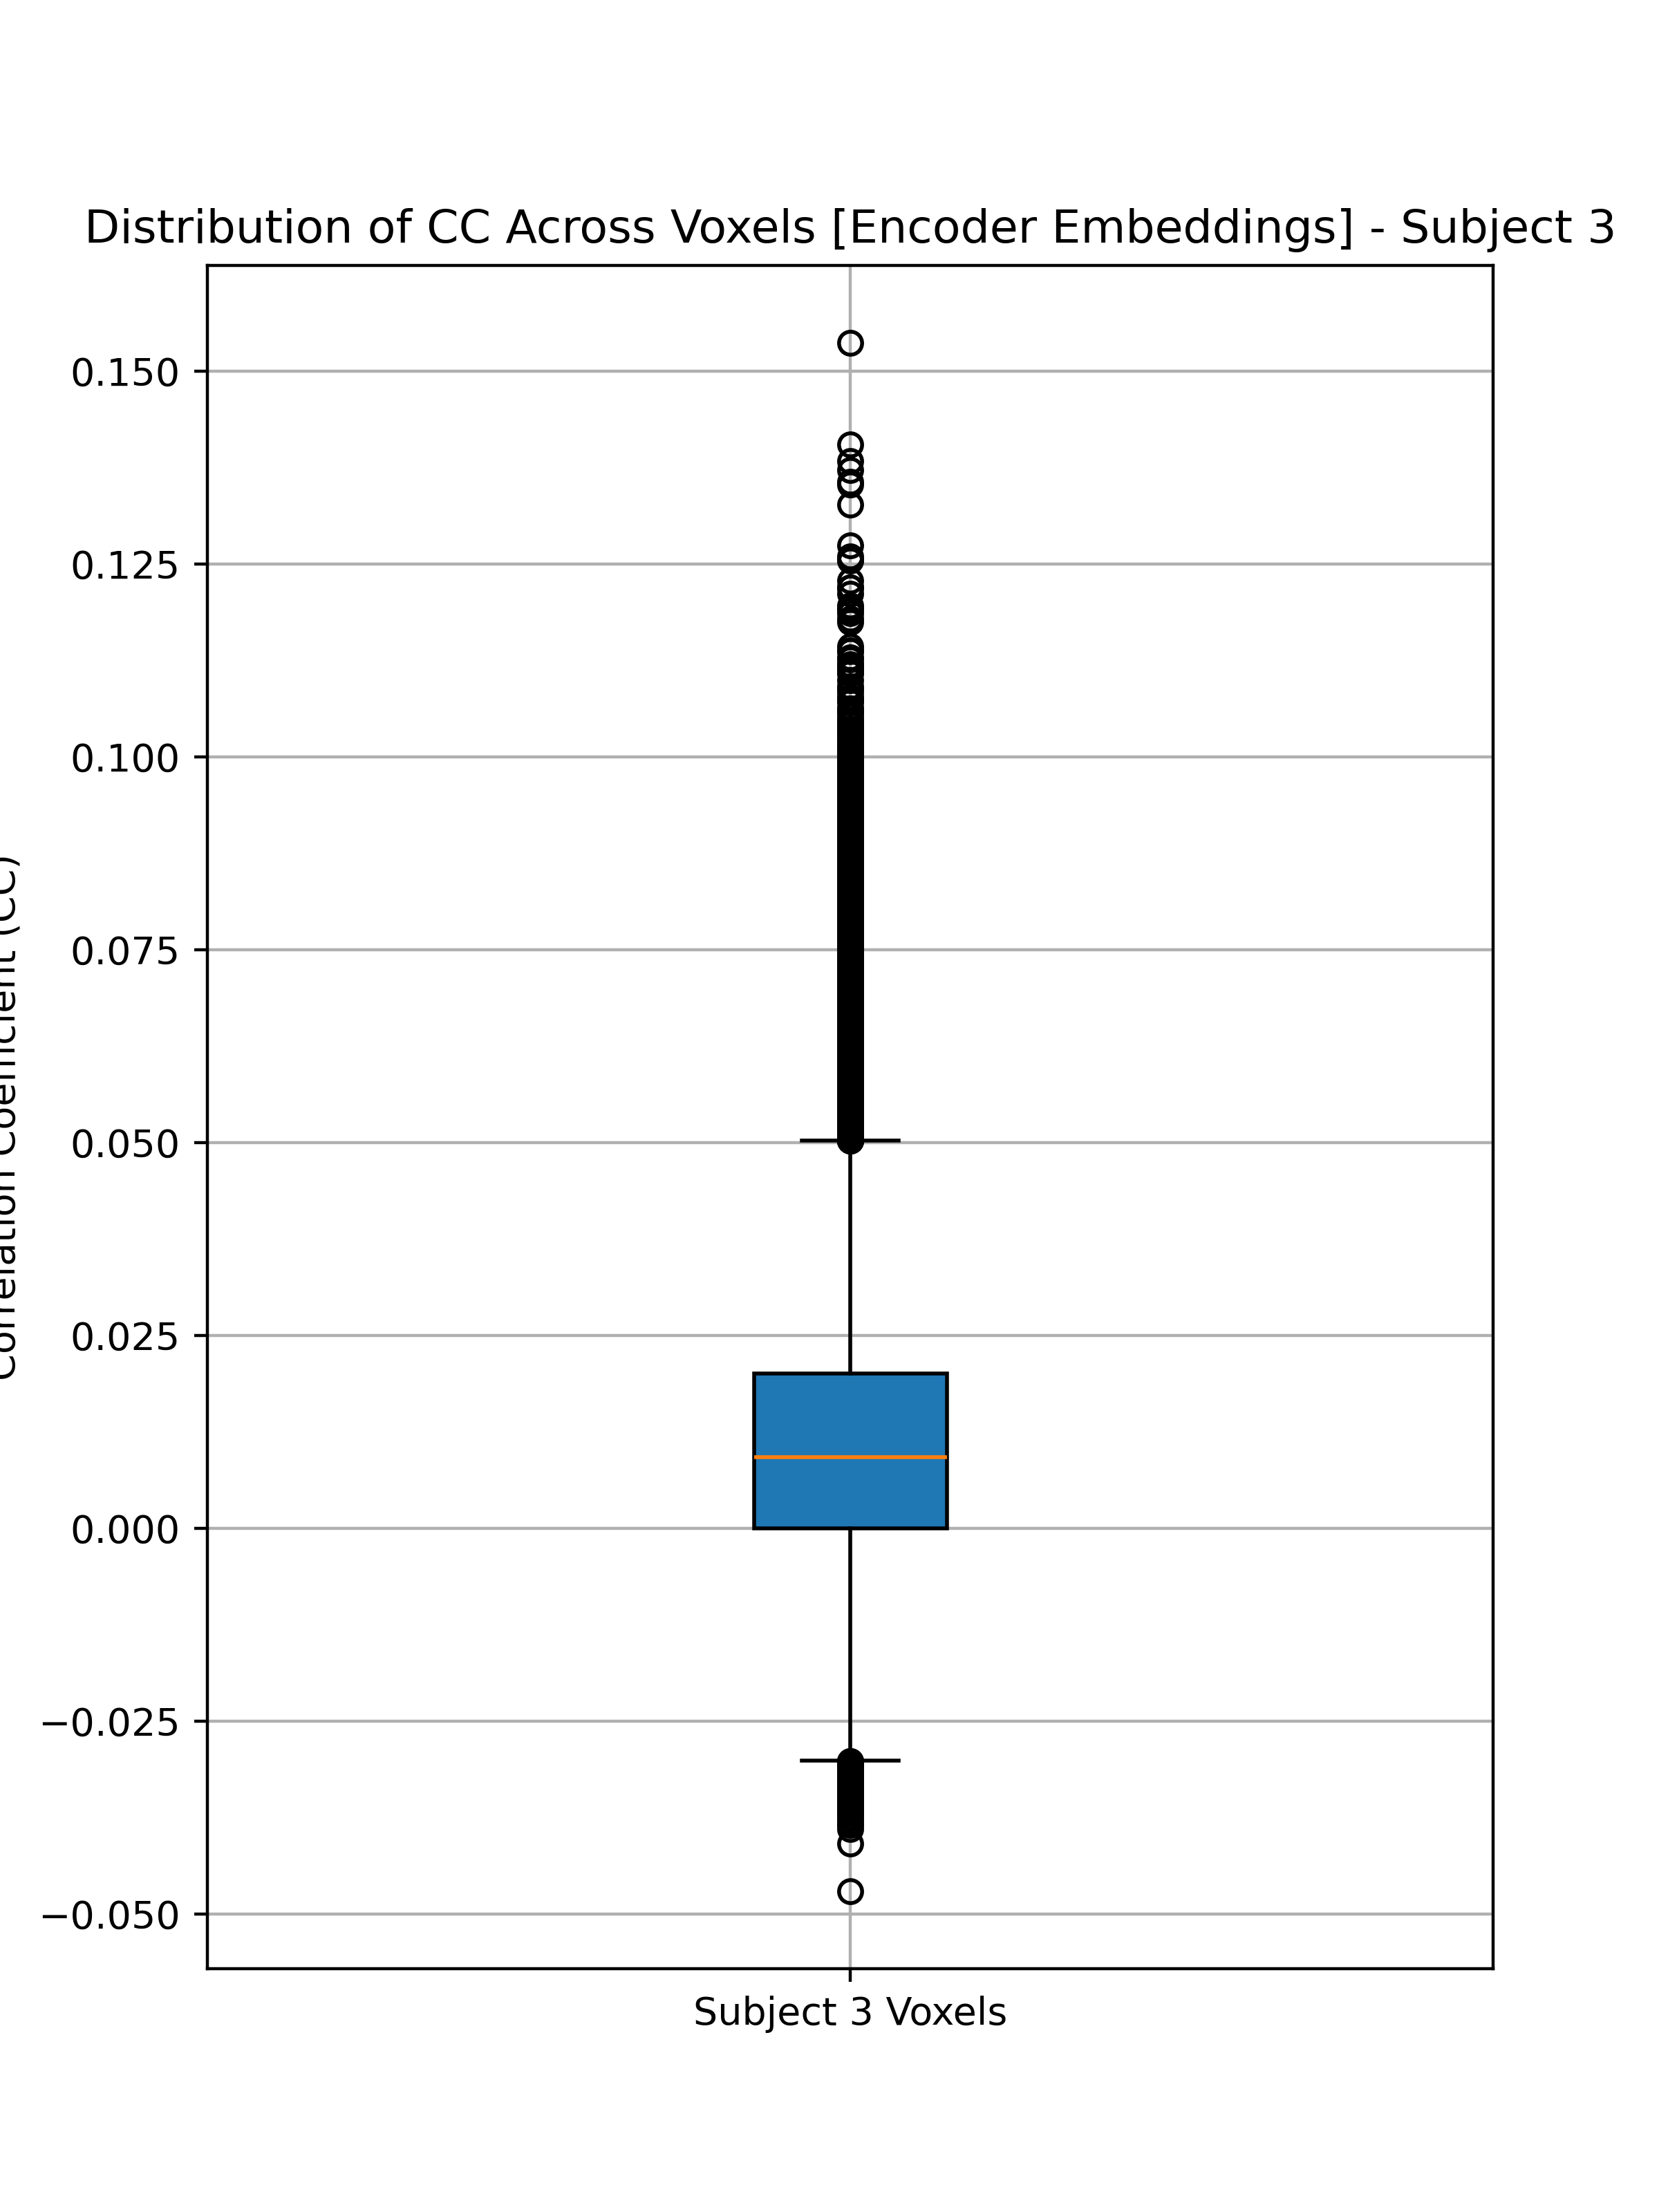
\includegraphics[width=0.5\linewidth]{figs/encoder_subj3_cc_dist.png}
    \caption{Distribution of CC across voxels for Subject 3 using Encoder embeddings.}
    \label{fig:cc_dist_encoder_subj_3}
\end{figure}

\section{Modeling - Pre-Trained BERT and LoRA}
In this section, we fit predictive models using the pre-trained BERT, both with a regression head only and finetuning the entire BERT with LoRA. We will compare the performance of these models to the previous models using pre-trained embeddings and encoder embeddings.

\subsection{Model Selection Criteria}

The core objective of our modeling phase is to predict fMRI voxel activity using features derived from textual stimuli. To evaluate and select the best-performing models, we employ a strategy largely consistent with previous labs, using story-level splits and focusing on the model's ability to generalize to unseen data. The primary metric for this evaluation remains the performance (measured by CC) on a held-out validation set.

A key departure from Lab 3.1 and 3.2 in our model selection process for this lab (Lab 3.3) is the shift from k-fold CV to a fixed train-validation-test split. Specifically, the available stories are divided into a training set (60\% of stories), a validation set (20\%), and a test set (20\%).

The rationale for using a validation set instead of k-fold CV is twofold:
\begin{enumerate}
    \item \textbf{Computational Cost:} Fine-tuning BERT, even with LoRA, is expensive. Performing k-fold CV would multiply this already significant computational burden by a factor of $k$, making extensive hyperparameter tuning or model exploration prohibitively expensive.
    \item \textbf{Early Stopping in Deep Learning:} A common and crucial practice in training deep learning models is early stopping. This technique involves monitoring the model's performance on a validation set and picking the model state that achieves the best performance on this set. Implementing a clear and consistent early stopping mechanism is more straightforward with a single, fixed validation set than within a k-fold CV framework because each fold in a CV may pick a different model state based on its own validation set performance.
\end{enumerate}

Therefore, for both modeling approaches in this section, model selection and hyperparameter tuning are guided by MSE loss on the fixed validation set. The model configuration that yields the lowest validation MSE for each subject is selected as the best-performing model for that subject. The final evaluation of these selected models is then performed on the reserved test set. This approach allows for practical model development while still providing a robust mechanism for generalization assessment and overfitting mitigation.

\subsection{Regression Head with Pretrained BERT Embeddings}

In this initial modeling phase, we utilize the embeddings generated from the pre-trained BERT as fixed features to predict fMRI voxel activity. The BERT model itself is not fine-tuned at this stage; only a linear regression head is trained on top of these static BERT embeddings. The process for obtaining these TR-level features from the stories was detailed in the previous sections. Each TR is thus represented by a 768-dimensional vector (the hidden size of BERT).

For each subject, a separate linear regression model is trained to map these 768-dimensional TR-level feature vectors to the BOLD signal activity across all their respective voxels.

Given the large number of features and target voxels, and consistent with common practices for training neural network components, we employ gradient descent to optimize the weights of these linear regression heads. This contrasts with the closed-form solution often used for traditional ridge regression when the dataset size allows. Instead of an explicit L2 penalty term in the loss function (as in standard ridge regression), we achieve regularization through weight decay in the optimizer.

The training procedure for these regression heads is as follows:
\begin{itemize}
    \item \textbf{Optimizer:} AdamW \cite{loshchilov2017decoupled} is used, incorporating weight decay directly into the optimization step, acting as L2 regularization.
    \item \textbf{Learning Rate:} A learning rate of $2 \times 10^{-3}$ was employed.
    \item \textbf{Weight Decay:} To investigate the impact of regularization, we experimented with three different weight decay values: $10^{-1}$, $10^{-2}$, and $10^{-3}$.
    \item \textbf{Loss Function:} MSE between the predicted and actual fMRI signals for each subject.
    \item \textbf{Epochs and Early Stopping:} The models were trained for a maximum of 100 epochs. The state of the linear regression head that achieved the lowest MSE on the validation set was saved as the best model for each subject. This early stopping mechanism helps prevent overfitting.
\end{itemize}

The performance of the best models will be evaluated on the test set in the following sections.

\subsection{LoRA Fine-tuning of BERT}

To further adapt the pre-trained BERT model to our specific fMRI prediction task, we employ Low-Rank Adaptation (LoRA) \cite{hu2021lora}, a parameter-efficient fine-tuning technique. Instead of updating all the weights of the large BERT model, LoRA introduces small, trainable low-rank matrices into specific layers, significantly reducing the number of trainable parameters while often achieving performance comparable to full fine-tuning. The original weights of the BERT model remain frozen.

The embedding extraction process remains unchanged from the previous section, where we used the pre-trained BERT model to generate TR-level features. The only difference is that we now propagate gradients through the embedding extraction pipeline and capture the gradients of the LoRA parameters. This is possible because the extraction pipeline is fully differentiable.

The LoRA configuration and training procedure are as follows:
\begin{itemize}
    \item \textbf{LoRA Target Modules:} We applied LoRA to the query and value projection matrices within each attention layer of the BERT model. The key and feed-forward dense layers were not modified with LoRA adapters in this setup, aligning with the standard practice in LoRA finetuning.
    \item \textbf{LoRA Rank (\(r\)):} We experimented with two LoRA ranks: \(r=4\) and \(r=8\). A lower rank results in fewer trainable parameters.
    \item \textbf{LoRA Alpha (\(\alpha\)):} The LoRA scaling factor \(\alpha\) was set to \(2 \times r\), a common practice in LoRA.
    \item \textbf{LoRA Dropout:} A dropout rate of \(0.1\) was applied to the LoRA layers.
    \item \textbf{Bias Term for LoRA:} No bias term was added to the LoRA layers, nor was the bias term in the original BERT model modified.
\end{itemize}

For the regression heads (the linear layers mapping the 768-dimensional BERT output to voxel activities for each subject), we initialized them with the weights obtained from the best-performing "Regression Head" trained in the previous section, with a weight decay of \(10^{-1}\). This initialization strategy is intended to leverage the knowledge learned during the regression head training phase, providing a warm start for the classifiers, preventing the BERT's weights from being breaked by the regression head training.

The joint optimization of LoRA parameters and the (initialized) regression heads followed this procedure:
\begin{itemize}
    \item \textbf{Optimizer:} AdamW \cite{loshchilov2017decoupled}.
    \item \textbf{Learning Rate:} A base learning rate of $2 \times 10^{-3}$ was used, scaled linearly by the ratio of the current batch size (15) to a reference batch size of 75.
    \item \textbf{Weight Decay:} A weight decay of $10^{-1}$ was applied to all trainable parameters.
    \item \textbf{Training Data and Batching:} The model was trained on the designated training set (60\% of stories), processed in mini-batches of 15 stories. The order of stories was shuffled at the beginning of each epoch.
    \item \textbf{Loss Function:} MSE between predicted and actual fMRI signals.
    \item \textbf{Epochs and Early Stopping:} Training proceeded for a maximum of 100 epochs. For each subject, the LoRA adapter weights and the corresponding regression head weights that yielded the lowest MSE on the validation set were saved independently.
\end{itemize}

The performance of the best models will be evaluated on the test set in the following sections.

\subsection{Model Comparison - Pre-trained vs Fine-tuned (LORA)}
In this section, we compare the performance of the pre-trained BERT model vs the model that we finetune using LORA. The results for CC across voxels, split by various metrics like Mean, Median, Top 1\%, and Top 5\% CC, are highlighted in Table \ref{tab:cc_subject2_comparison_finetuned_vs_pretrained}. We consider these different metrics (as in prior labs) to have a more robust sense of how the models are performing across voxels, and whether certain models have more variance in their voxel performance.

We can see that overall, fine-tuning does improve the performance of the model as expected. However, the improvement is very relatively small in magnitude. For subject 2, the Mean CC improves by around 0.002, which represents an approximately 10\% change. The upper echelons of voxels in terms of performance, meaning the Top 10\% and Top 5\% CC's, improve by a smaller relative change. Overall, we see a notable but small improvement performance across voxels, both throughout the mean/median and the best-performing voxels.

These experiments are repeated for Subject 3 in Table \ref{tab:cc_subject3_comparison_finetuned_vs_pretrained}. We generally see the same takeaways, just with consistenly worse performances across both models and all metrics. This may indicate that it is harder to predict fMRI levels for Subject 3. Another note is that the improvement between pretrained and finetuned at the top-performing voxels for Subject 3 is relatively smaller than the improvement we see in Subject 2.


\begin{table}[ht]
\centering
\caption{Voxel-wise test-set correlation (CC) for Subject 2: fine-tuned vs.\ pretrained model}
\label{tab:cc_subject2_comparison_finetuned_vs_pretrained}
\begin{tabular}{lcccc}
\toprule
\textbf{Model} & \textbf{Mean CC} & \textbf{Median CC} & \textbf{Top 1\% CC} & \textbf{Top 5\% CC} \\
\midrule
Pretrained & 0.018732 & 0.014398 & 0.103731 & 0.064962 \\
Fine–tuned & 0.020627 & 0.015985 & 0.108326 & 0.069247 \\
\bottomrule
\end{tabular}
\end{table}


\begin{table}[h!]
\centering
\caption{Voxel-wise test-set correlation (CC) for Subject 3: fine-tuned vs. pretrained model}
\label{tab:cc_subject3_comparison_finetuned_vs_pretrained}
\begin{tabular}{lcccc}
\toprule
\textbf{Model} & \textbf{Mean CC} & \textbf{Median CC} & \textbf{Top 1\% CC} & \textbf{Top 5\% CC} \\
\midrule
Pretrained & 0.005317 & 0.005367 & 0.044171 & 0.030436 \\
Fine–tuned & 0.005947 & 0.005888 & 0.045137 & 0.031242 \\
\bottomrule
\end{tabular}
\end{table}



Additionally, we wanted to explore in greater depth how performance looks across the distribution of voxels for each model. These can be compared through a histogram of the CC distribution across voxels, shown in Figure \ref{fig:cc_dist_pretrained_finetuned_subj2}. Through this, we can see that both the pretrained and finetuned model CC's follow roughly the same distribution in shape. The pretrained model, however, has a higher concentration of CC around the 0.01 region.


\begin{figure}[ht]
    \centering
    
    \begin{subfigure}[t]{0.4\textwidth}
        \centering
        \caption{Pre-trained Model}
        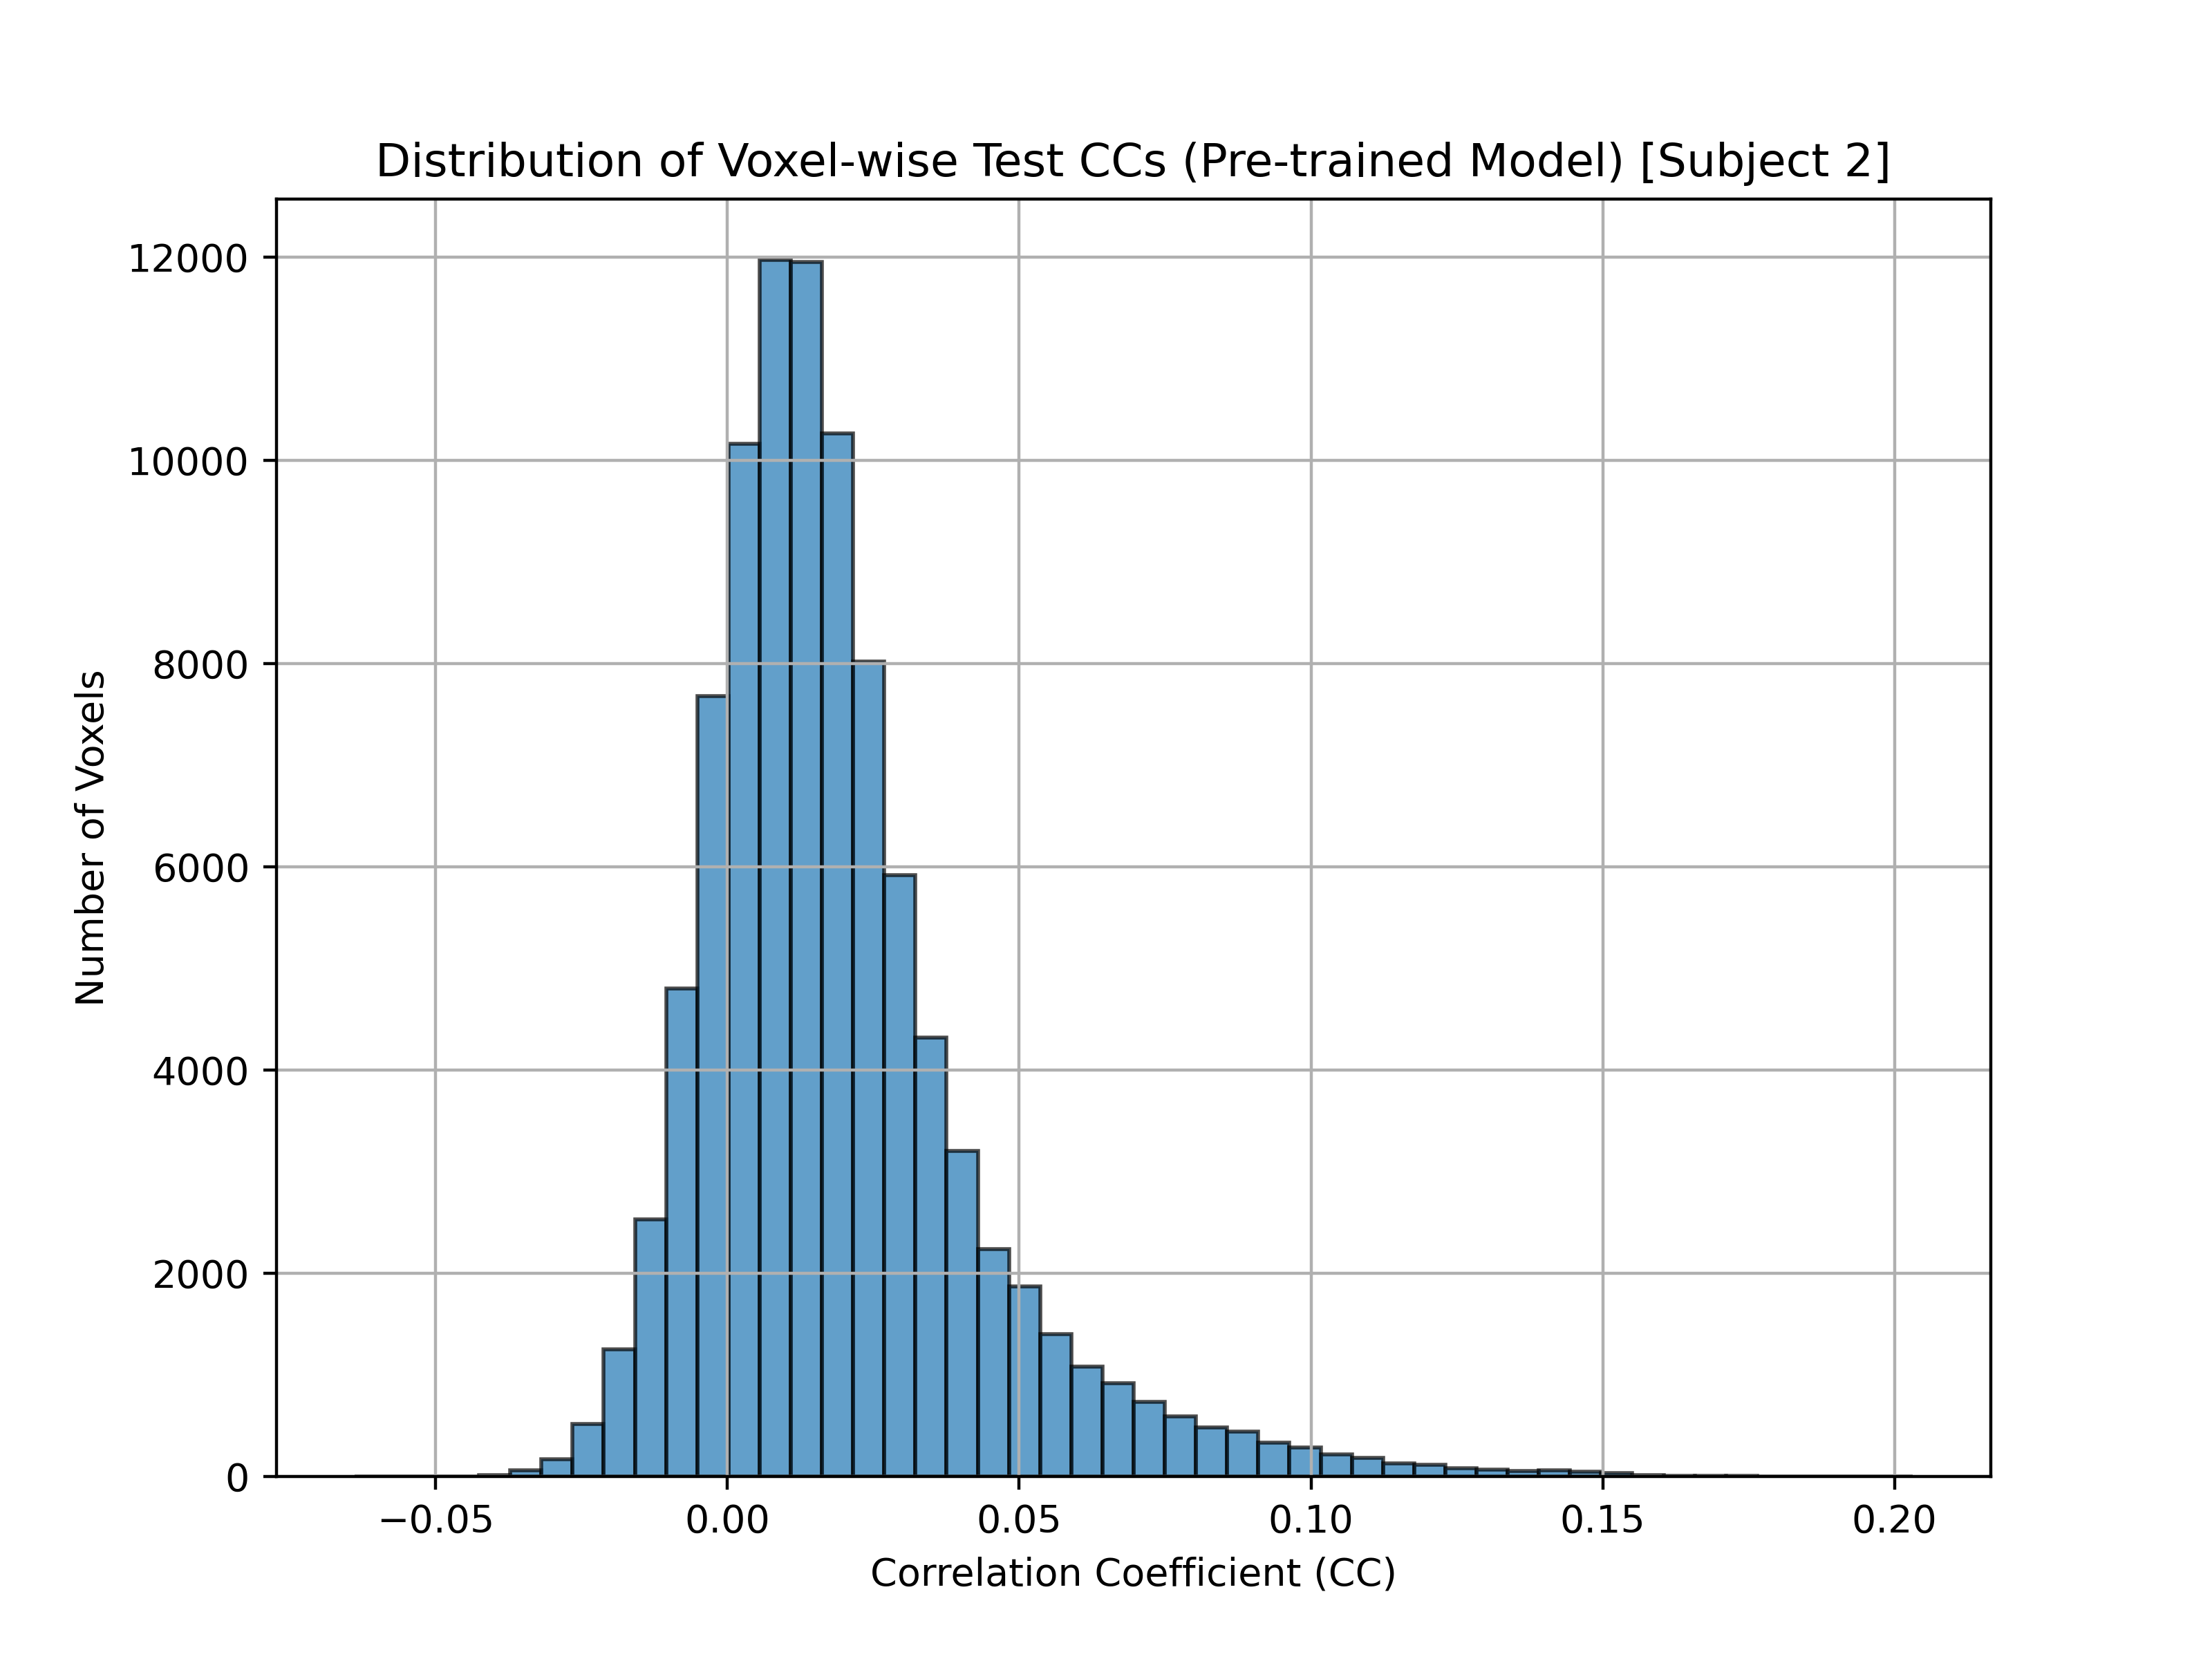
\includegraphics[width=\textwidth]{figs/cc_dist_pretrained_subj2.png}
        \label{fig:cc_dist_pretrained_subj2}
    \end{subfigure}
    \hfill
    \begin{subfigure}[t]{0.4\textwidth}
        \centering
        \caption{Fine-tuned Model}
        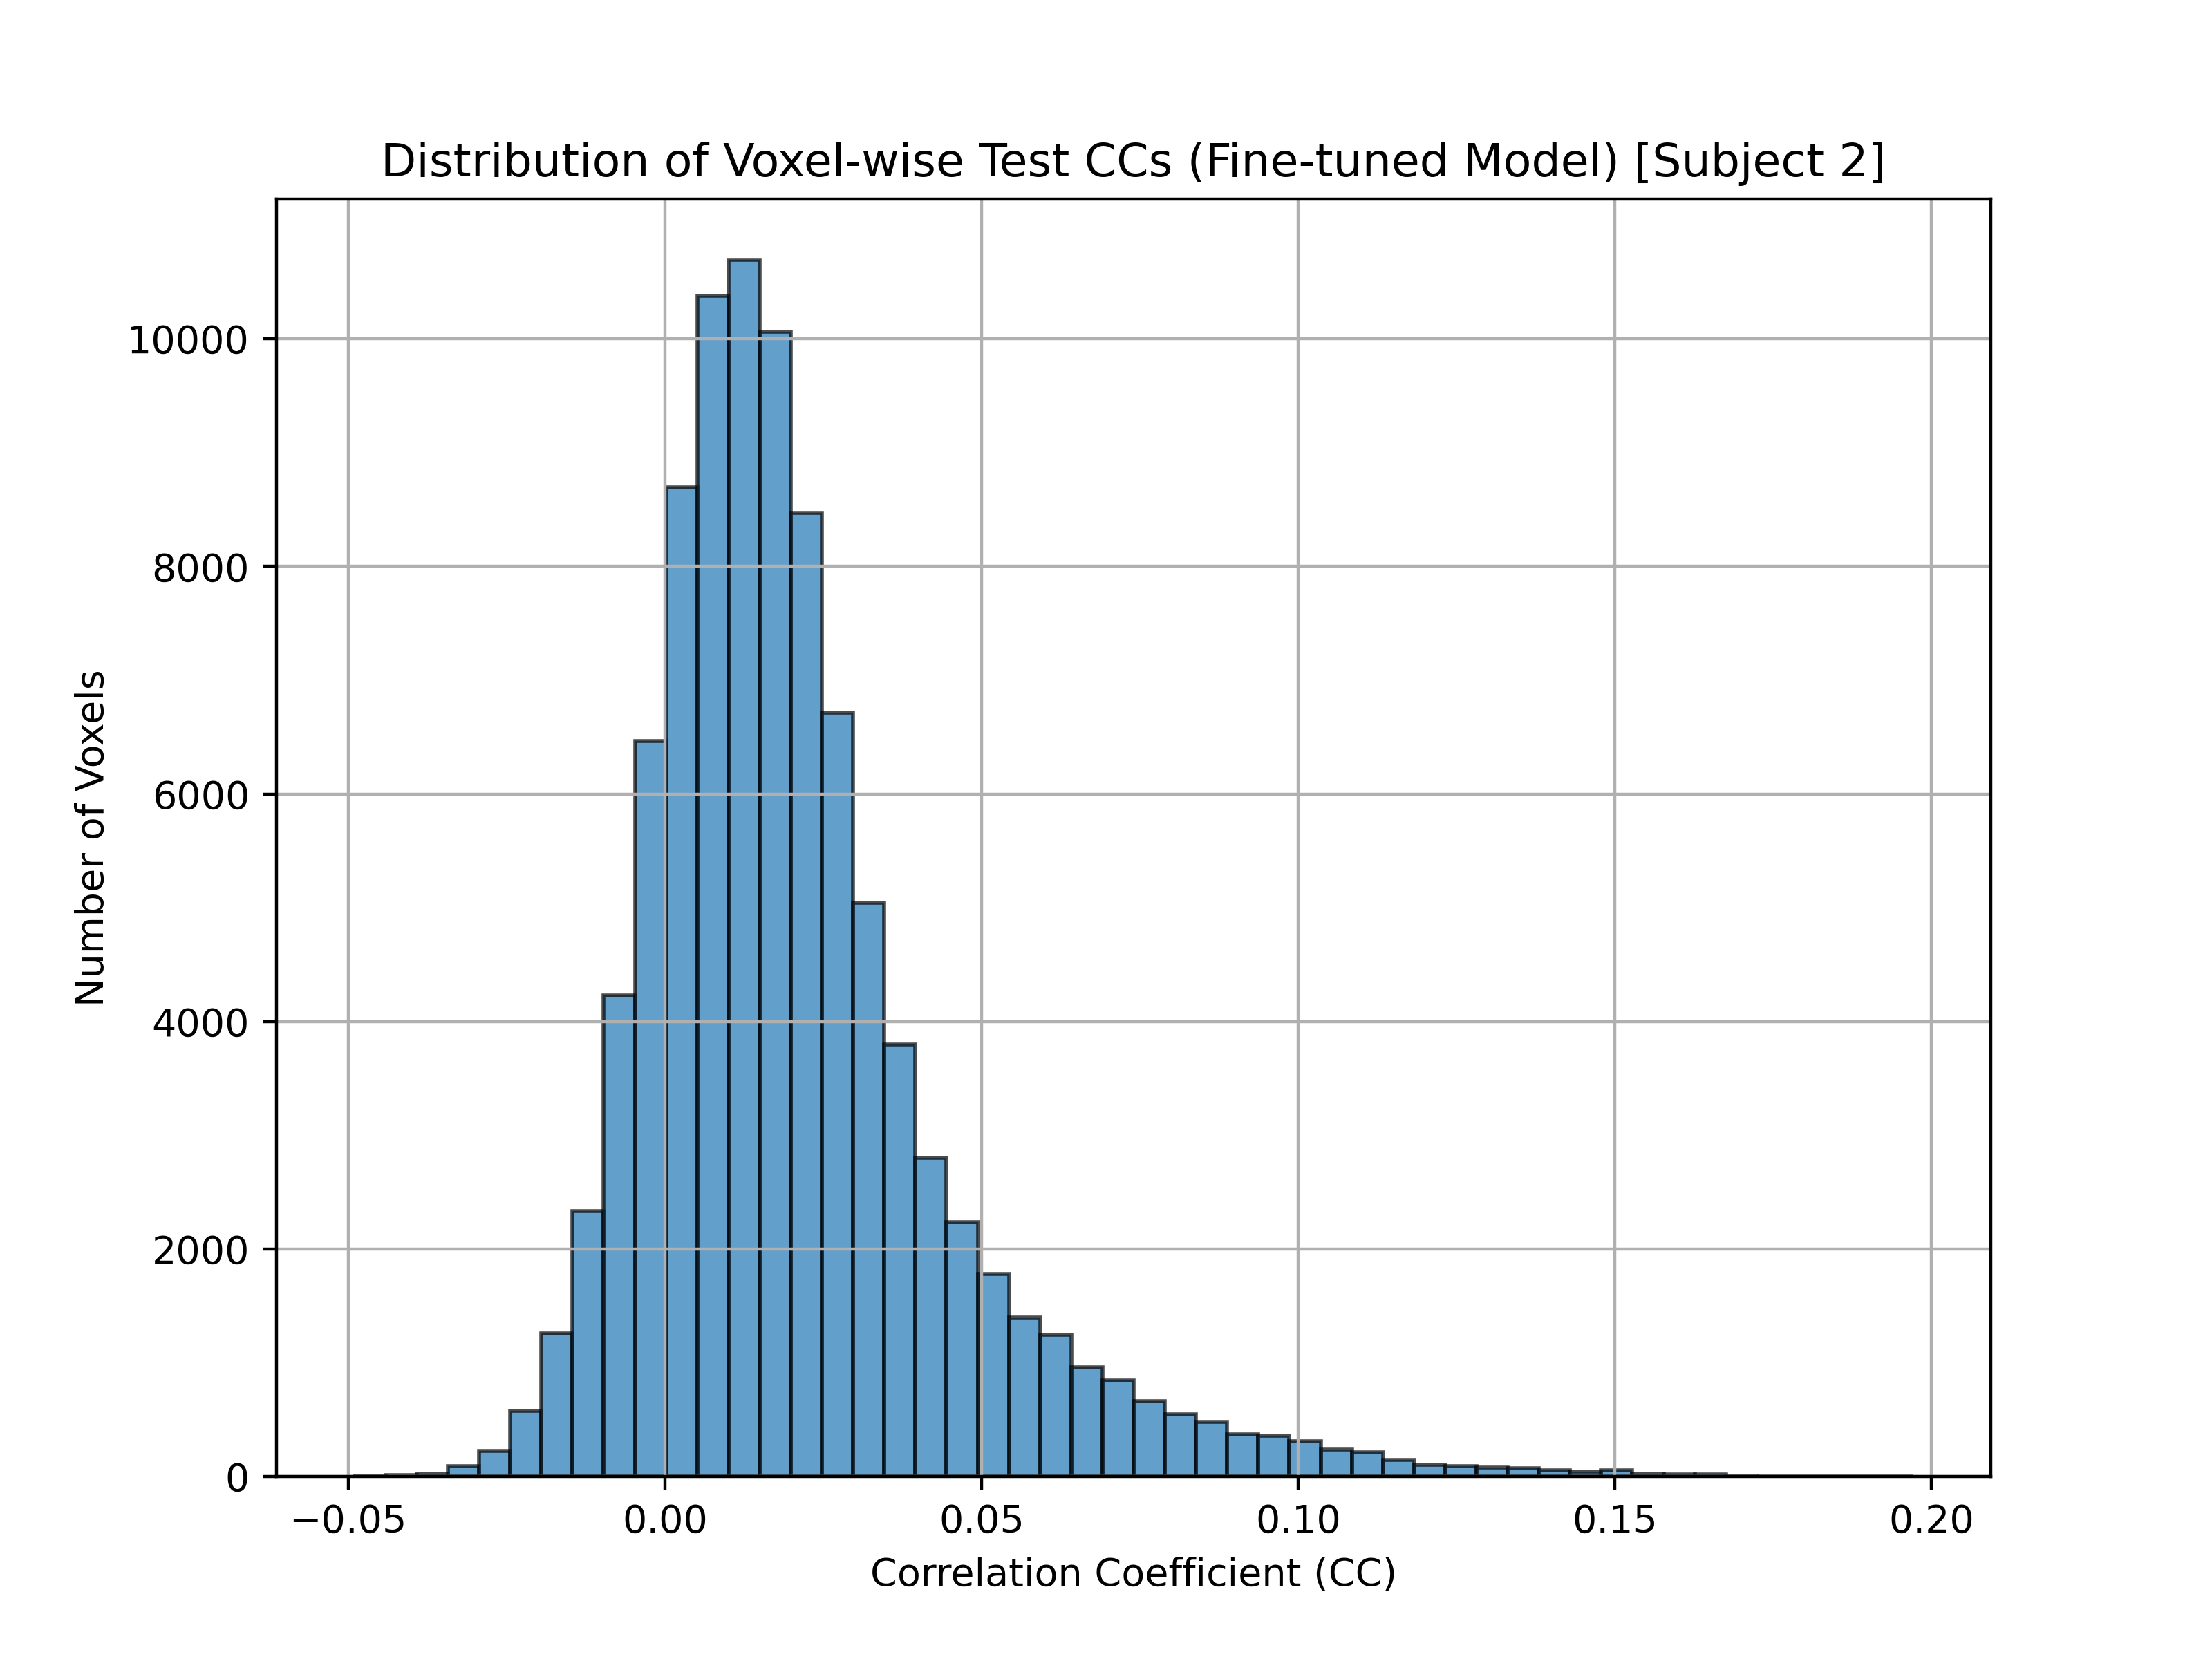
\includegraphics[width=\textwidth]{figs/cc_dist_finetuned_subj2.png}
        \label{fig:cc_dist_finetuned_subj2}
    \end{subfigure}

    \caption{Test CC Distribution for the Pre-trained Model (left) and Fine-tuned Model (right) for Subject 2.}
    \label{fig:cc_dist_pretrained_finetuned_subj2}
\end{figure}



\subsection{Model Comparison - All Models}
We now compare the performance of the fine-tuned model and pre-trained model with all models from parts 3.1 and 3.2. This includes the model with encoder embeddings, Word2Vec, GloVe, and Bag of Words. The results are shown in Table \ref{tab:cc_subject2_full}

\begin{table}[ht]
\centering
\caption{Voxel-wise test-set correlation coefficients (CC) for \textbf{Subject 2}.}
\label{tab:cc_subject2_full}
\begin{tabular}{lcccc}
\toprule
\textbf{Model} &
\textbf{Mean CC} &
\textbf{Median CC} &
\textbf{Top 1\% CC} &
\textbf{Top 5\% CC} \\
\midrule
Finetuned  & 0.020627 & 0.015985 & 0.108326 & 0.069247 \\
Pretrained & 0.018732 & 0.014398 & 0.103731 & 0.064962 \\
Encoder    & 0.005989 & 0.005274 & 0.041602 & 0.029038 \\
Word2Vec   & 0.005648 & 0.004466 & 0.050116 & 0.032150 \\
GloVe      & 0.004951 & 0.004253 & 0.043254 & 0.029343 \\
BoW        & 0.000904 & 0.000870 & 0.031131 & 0.021515 \\
\bottomrule
\end{tabular}
\end{table}

For the purpose of stability and completeness of our analysis, this comparison was repeated for Subject 3. These results are shown in Table \ref{tab:cc_subject3_full}.



\begin{table}[ht]
\centering
\caption{Voxel-wise test-set correlation coefficients (CC) for \textbf{Subject 3}.}
\label{tab:cc_subject3_full}
\begin{tabular}{lcccc}
\toprule
\textbf{Model} &
\textbf{Mean CC} &
\textbf{Median CC} &
\textbf{Top 1\% CC} &
\textbf{Top 5\% CC} \\
\midrule
Finetuned  & 0.005947 & 0.005888 & 0.045137 & 0.031242 \\
Pretrained & 0.005317 & 0.005367 & 0.044171 & 0.030436 \\
Encoder    & 0.011400 & 0.009270 & 0.068056 & 0.042578 \\
Word2Vec   & 0.008742 & 0.006996 & 0.062659 & 0.038738 \\
GloVe      & 0.008662 & 0.006905 & 0.061016 & 0.038540 \\
BoW        & 0.001653 & 0.001390 & 0.032009 & 0.021303 \\
\bottomrule
\end{tabular}
\end{table}


We also compare against the visual distributions of the previous models (in Labs 3.1 and 3.2) to understand the specific performance across voxels. We can see that the pretrained and finetuned models have a more skewed distribution than the previous models, which have a more centered distribution. In general, the previous models also exhibit lower performance than the pretrained and finetuned models, which have more parameters and are pretrained on a larger corpus. This is expected, as the pretrained and finetuned models are more complex and capable of capturing more complex patterns in natural language.

However, for Subject 3, the performance is quite different. The Encoder-based model, Word2Vec, and GloVe end up having better performance than the finetuned and pretrained models. This could indicate some instability in the result between the two subjects. Additionally, it could indicate that simpler baselines work better for Subject 3 prediction.

\begin{figure}[ht]
    \centering
    
    \begin{subfigure}[t]{0.4\textwidth}
        \centering
        \caption{Word2Vec Model}
        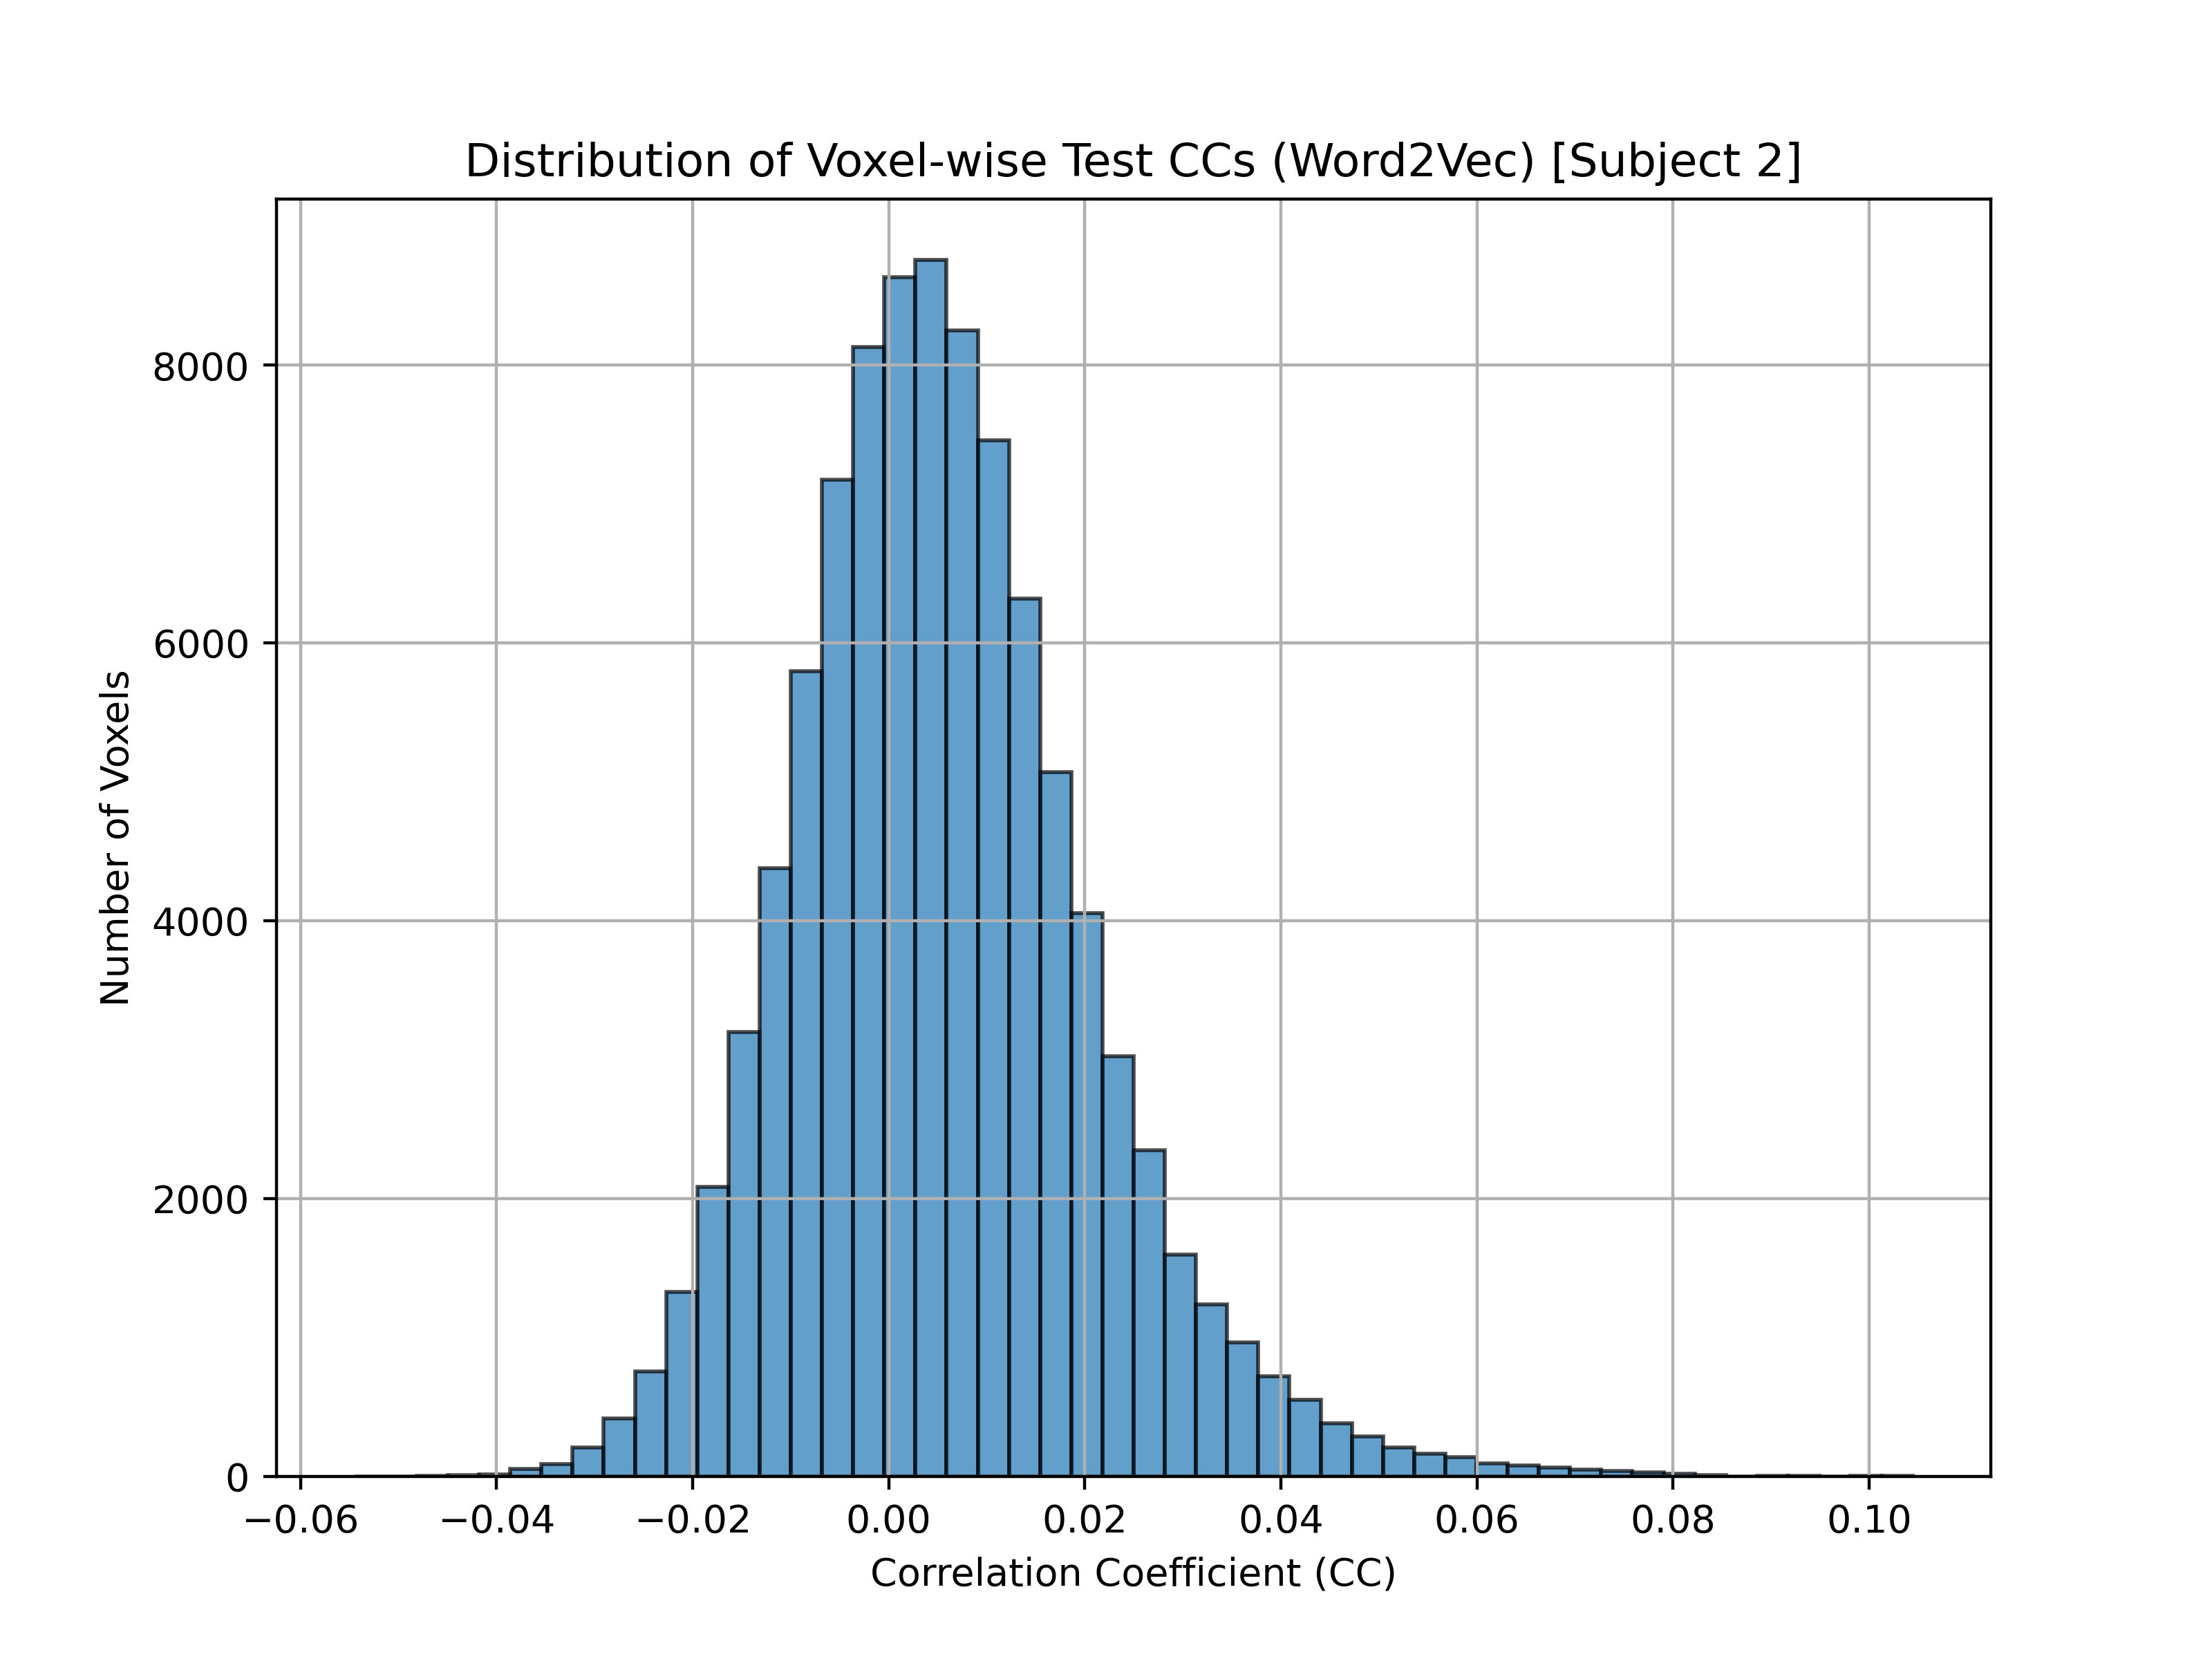
\includegraphics[width=\textwidth]{figs/cc_dist_Word2Vec.png}
        \label{fig:cc_dist_Word2Vec}
    \end{subfigure}
    \hfill
    \begin{subfigure}[t]{0.4\textwidth}
        \centering
        \caption{Encoder Model}
        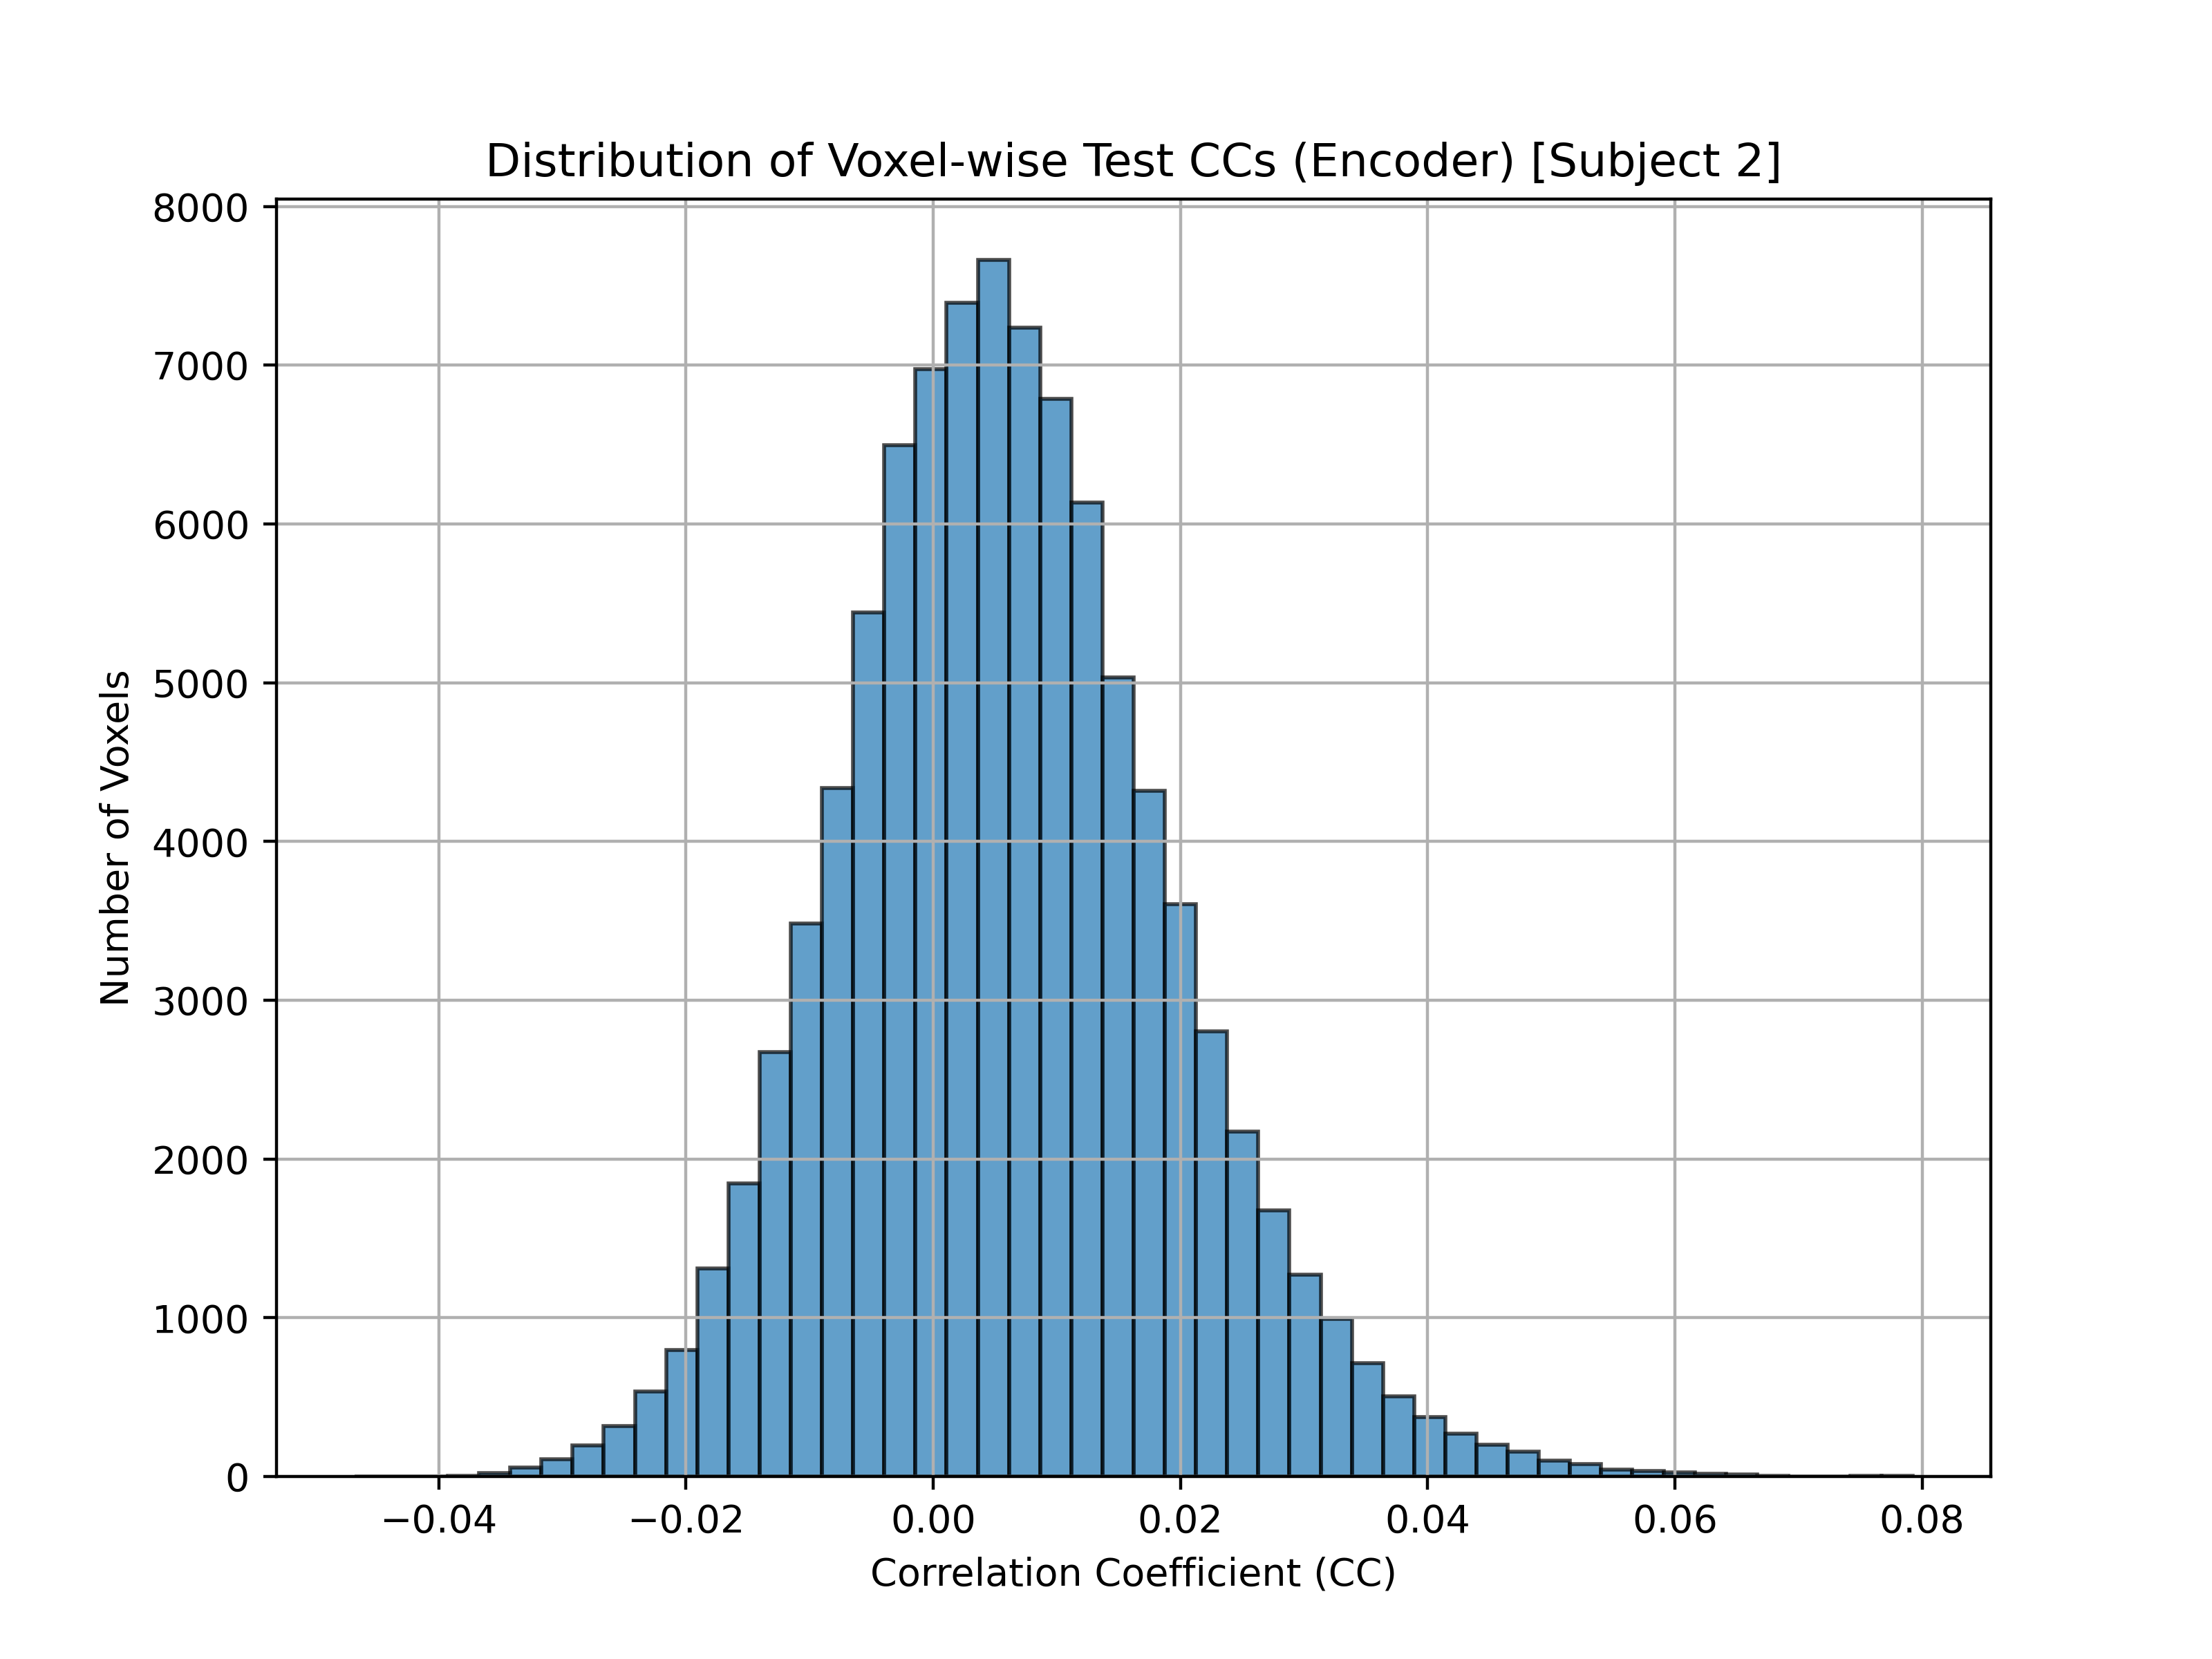
\includegraphics[width=\textwidth]{figs/cc_dist_Encoder.png}
        \label{fig:cc_dist_Encoder}
    \end{subfigure}

    \caption{Test CC Distribution for the Word2Vec Model (left) and Encoder Model (right) for Subject 2.}
    \label{fig:cc_dist_Word2Vec_Encoder}
\end{figure}

\newpage

\section{Interpretation}

In this section, we apply SHAP (SHapley Additive exPlanations) and LIME (Local Interpretable Model-agnostic Explanations) to interpret the fine-tuned BERT model's predictions by identifying the most influential words for two different test stories: \texttt{buck} and \texttt{lawsthatchokecreativity}. Annotated versions of each story, highlighting word-level importances, are included in Appendix \ref{sec:buck_text} and Appendix \ref{sec:laws_text}.

\subsection{Voxel Selection}

Although the fine-tuned model generates predictions for all $94{,}251$ voxels in Subject 2 and $95{,}556$ voxels in Subject 3, we limit our interpretability analysis to the voxels where the model performs well. This selective approach is crucial: methods like SHAP and LIME attempt to assign attribution based on a model's behavior, so they are only meaningful when the model's predictions are reliable. Interpreting poorly performing voxels would be misleading because feature attributions would reflect noise rather than a meaningful signal.

To identify the most informative voxels, we rank them by the CC between predicted and actual fMRI responses across time points. We then select voxels whose performance exceeds the 99.5th percentile (i.e., the top 0.5\% of correlation scores). Table \ref{tab:voxel_select} shows the corresponding CC thresholds for each subject and story. From the eligible voxels, we randomly sample a subset for SHAP and LIME interpretation to keep the analysis computationally manageable.


\begin{table}[ht]
    \centering
    \caption{Top 0.5\% CC Voxel Thresholds}
    \begin{tabular}{r|r|r}
        \toprule
        \textbf{Story}                   &  \textbf{Subject 2} & \textbf{Subject 3}\\
        \midrule
        \texttt{buck}                    &  0.216              & 0.294\\
        \hline
        \texttt{lawsthatchokecreativity} &  0.159              & 0.206\\
        \bottomrule
    \end{tabular}
    \label{tab:voxel_select}
\end{table}

\subsection{SHAP \& LIME Implementation}

Both SHAP and LIME explain model predictions by perturbing the input features and measuring how those changes affect the output, attributing influence to each feature accordingly. In our case, the model takes BERT embeddings as input and outputs fMRI predictions, so we define a wrapper function around the model that returns predictions only for a subset of high-performing voxels. This allows SHAP and LIME to focus their explanations on the most informative regions of the brain.

For SHAP, we use \texttt{KernelExplainer}, a model-agnostic method that estimates Shapley values by fitting a locally weighted linear model around each prediction. For LIME, we use \texttt{LimeTabularExplainer}, which similarly fits local linear models to approximate feature importances. Both methods require a background dataset to serve as a reference distribution for generating perturbed samples. To ensure consistency and interpretability, we use the BERT embeddings from several training set stories as the background.

After applying SHAP and LIME, we obtain a three-dimensional array of explanation values with shape \texttt{(num\_chunks, embedding\_dim, num\_voxels)}. To summarize these into word-level importance scores for each voxel, we take the absolute value of the explanation values and then average across the embedding dimension. The result is a matrix of shape \texttt{(num\_chunks, num\_voxels)} that reflects the relative importance of each word chunk to each voxel’s predicted activation.

\subsection{Test Story 1: \texttt{buck}}

As shown in Figure \ref{fig:scatter_buck_1}, the word rankings produced by SHAP and LIME for \texttt{buck} are fairly consistent between Subject 2 and Subject 3, although the correlation is weaker than that observed for the raw attribution scores. This suggests that both SHAP- and LIME-based word importances are relatively stable across listeners to this story.


\begin{figure}[ht]
    \centering

    \parbox{\textwidth}{\centering 
        \fontsize{13pt}{13pt}\selectfont \textbf{Cross-Subject Consistency in Word Importance}  
        
        {\fontsize{11pt}{13pt}\selectfont Comparing SHAP and LIME scores and ranks between Subject 2 and Subject 3} 
    }
    
    \begin{subfigure}[t]{0.22\textwidth}
        \centering
        \caption{SHAP Scores}
        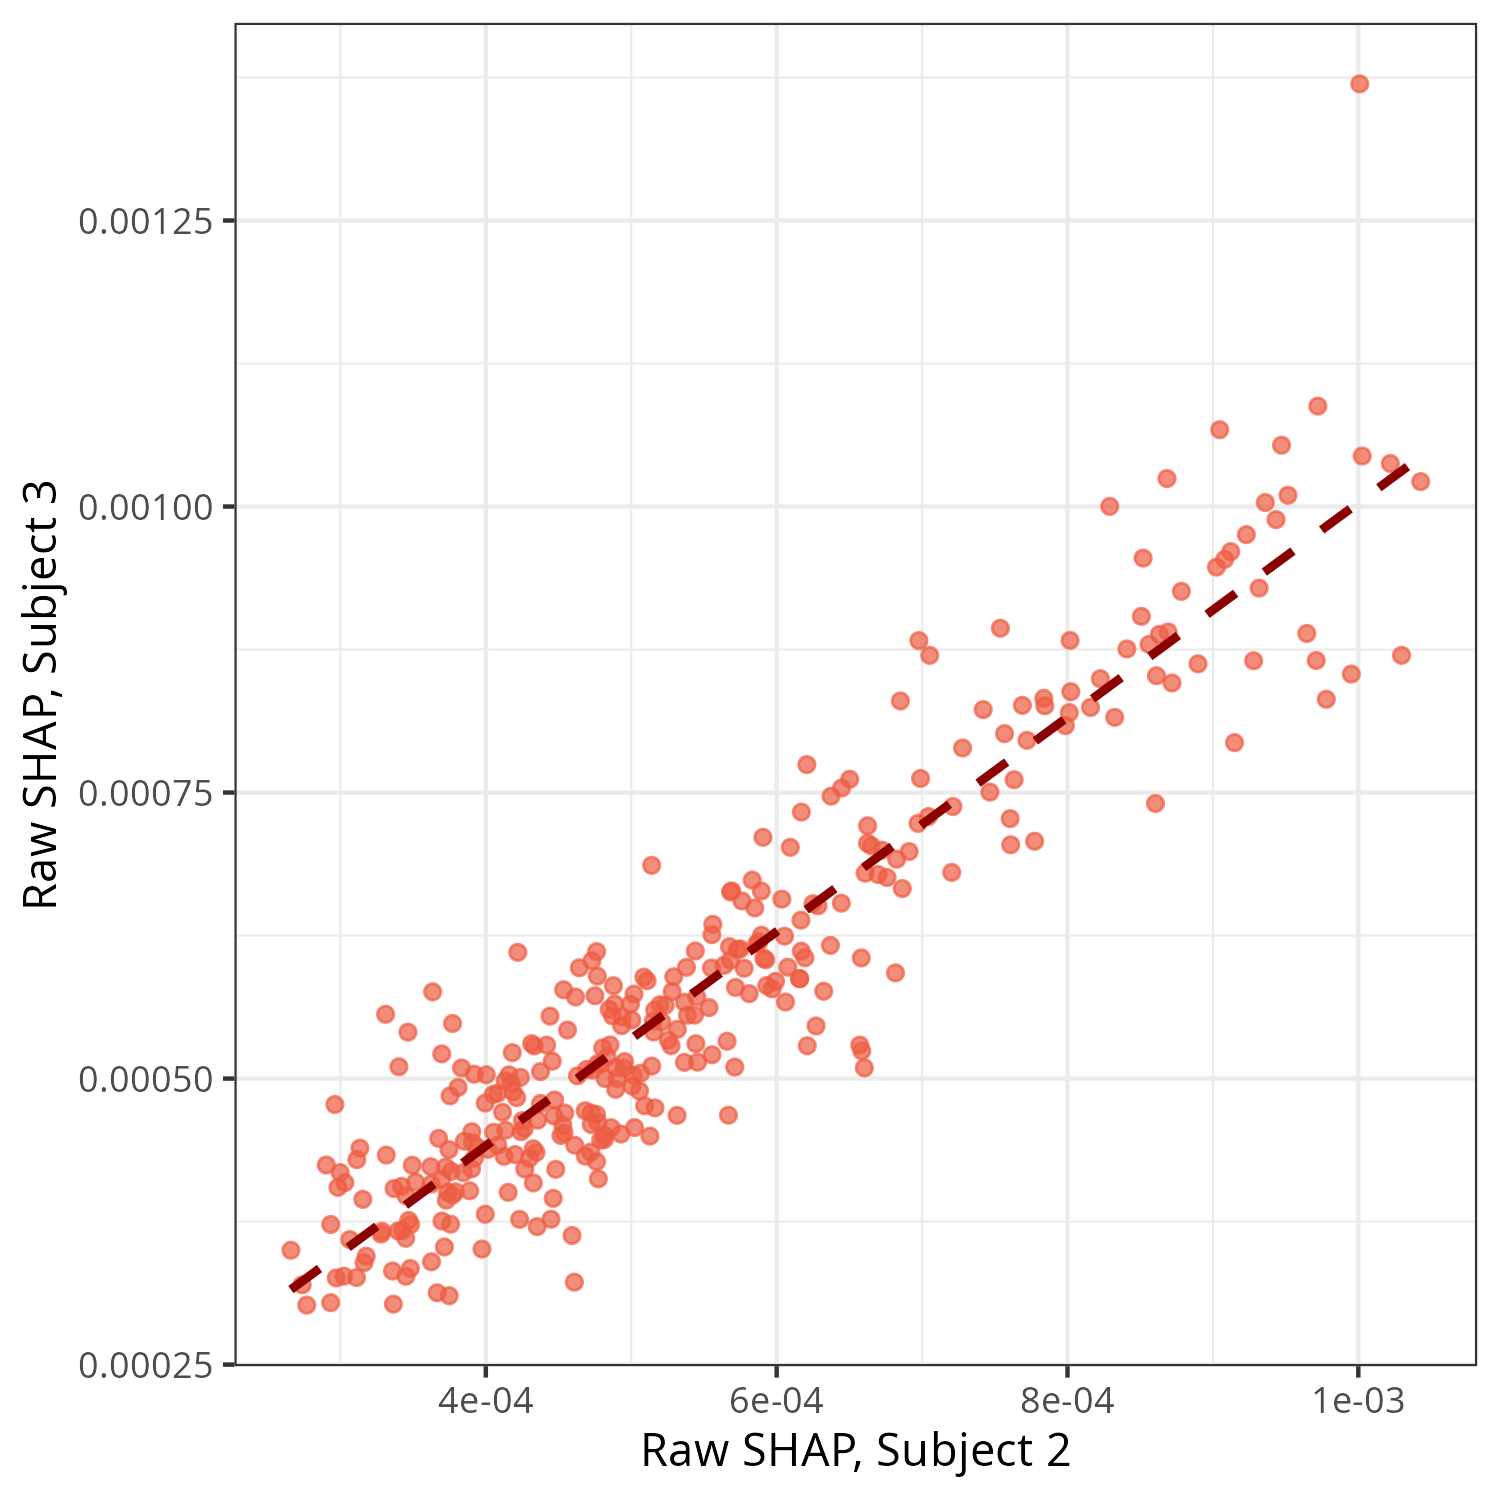
\includegraphics[width=\textwidth]{figs/scatter_buck_shap_raw.png}
        \label{subfig:scatter_buck_shap_raw}
    \end{subfigure}
    \hfill
    \begin{subfigure}[t]{0.22\textwidth}
        \centering
        \caption{SHAP Ranks}
        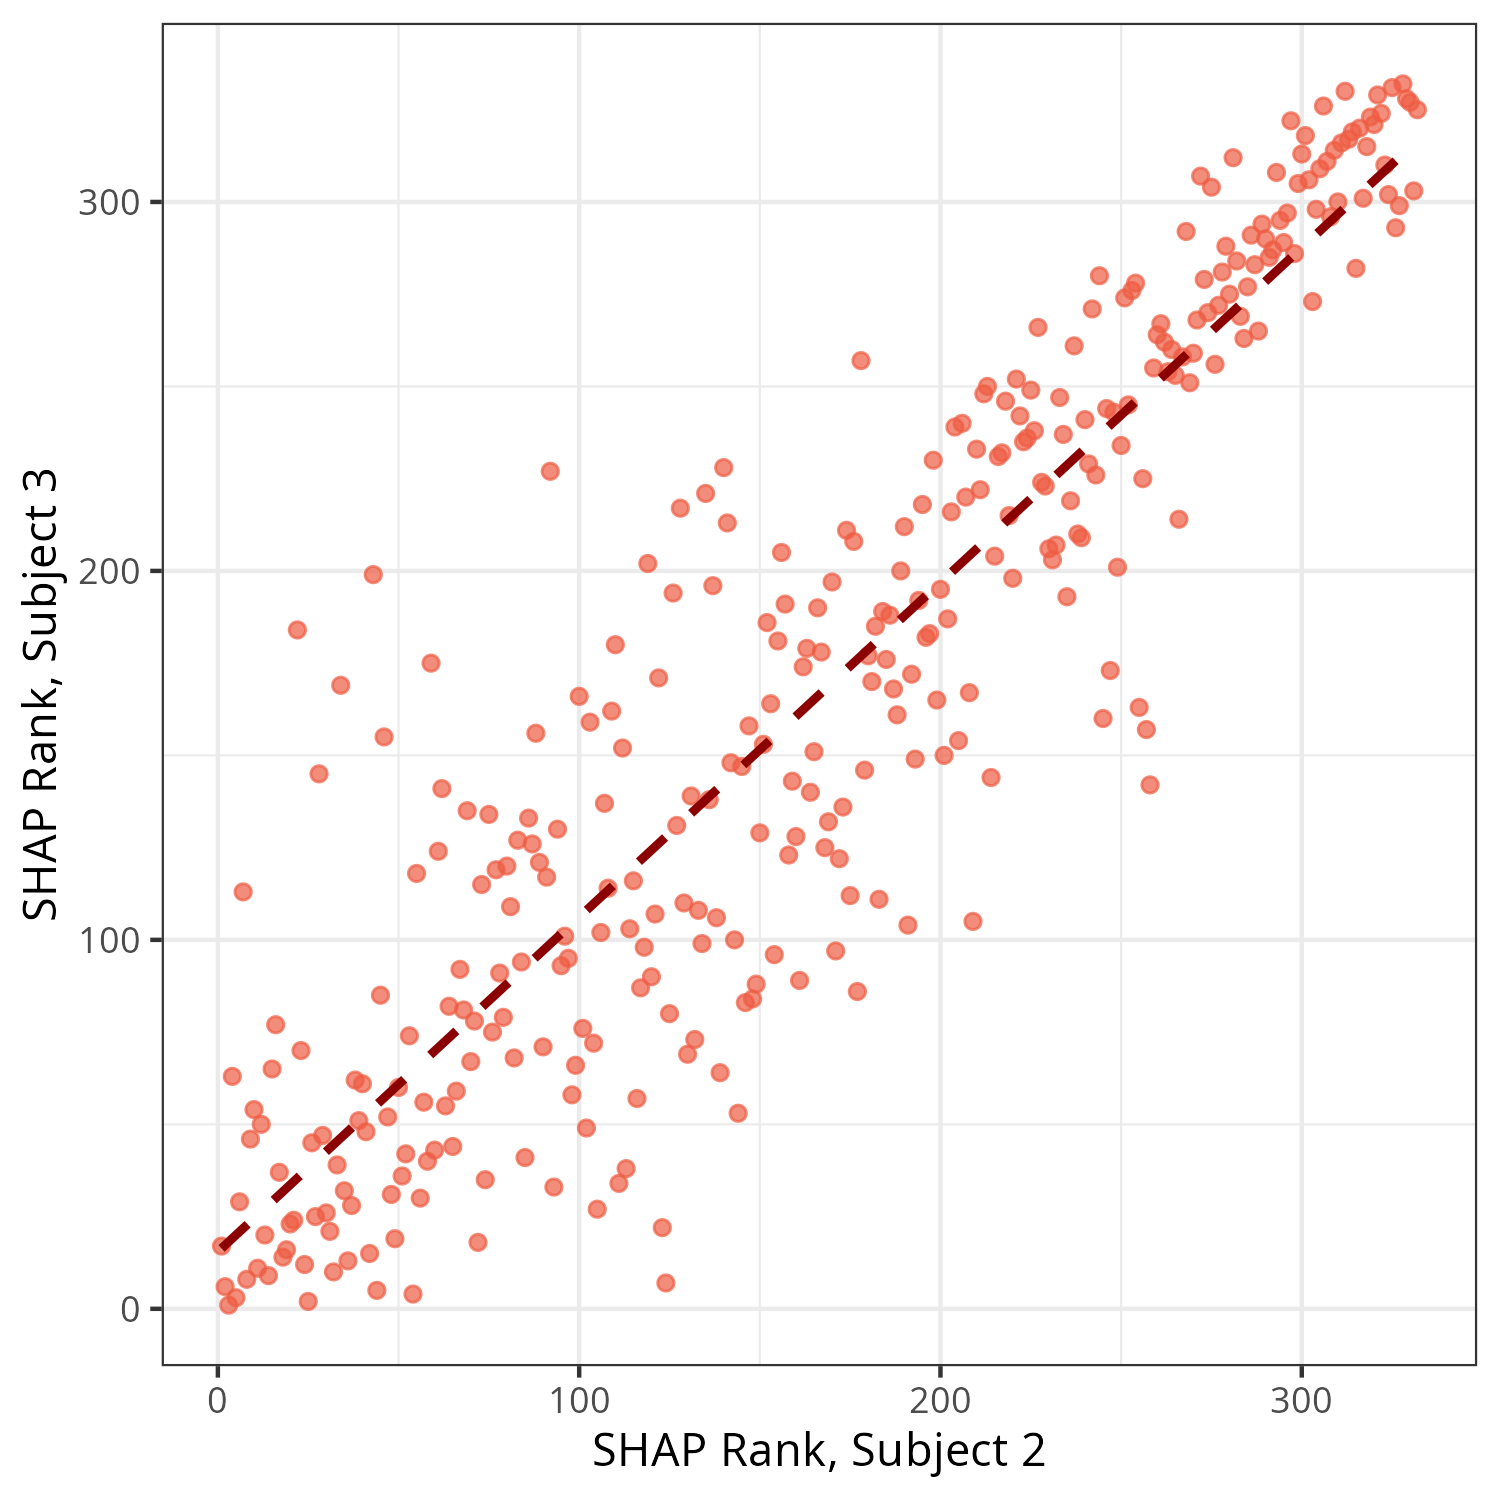
\includegraphics[width=\textwidth]{figs/scatter_buck_shap_rank.png}
        \label{subfig:scatter_buck_shap_rank}
    \end{subfigure}
    \hfill
    \begin{subfigure}[t]{0.22\textwidth}
        \centering
        \caption{LIME Scores}
        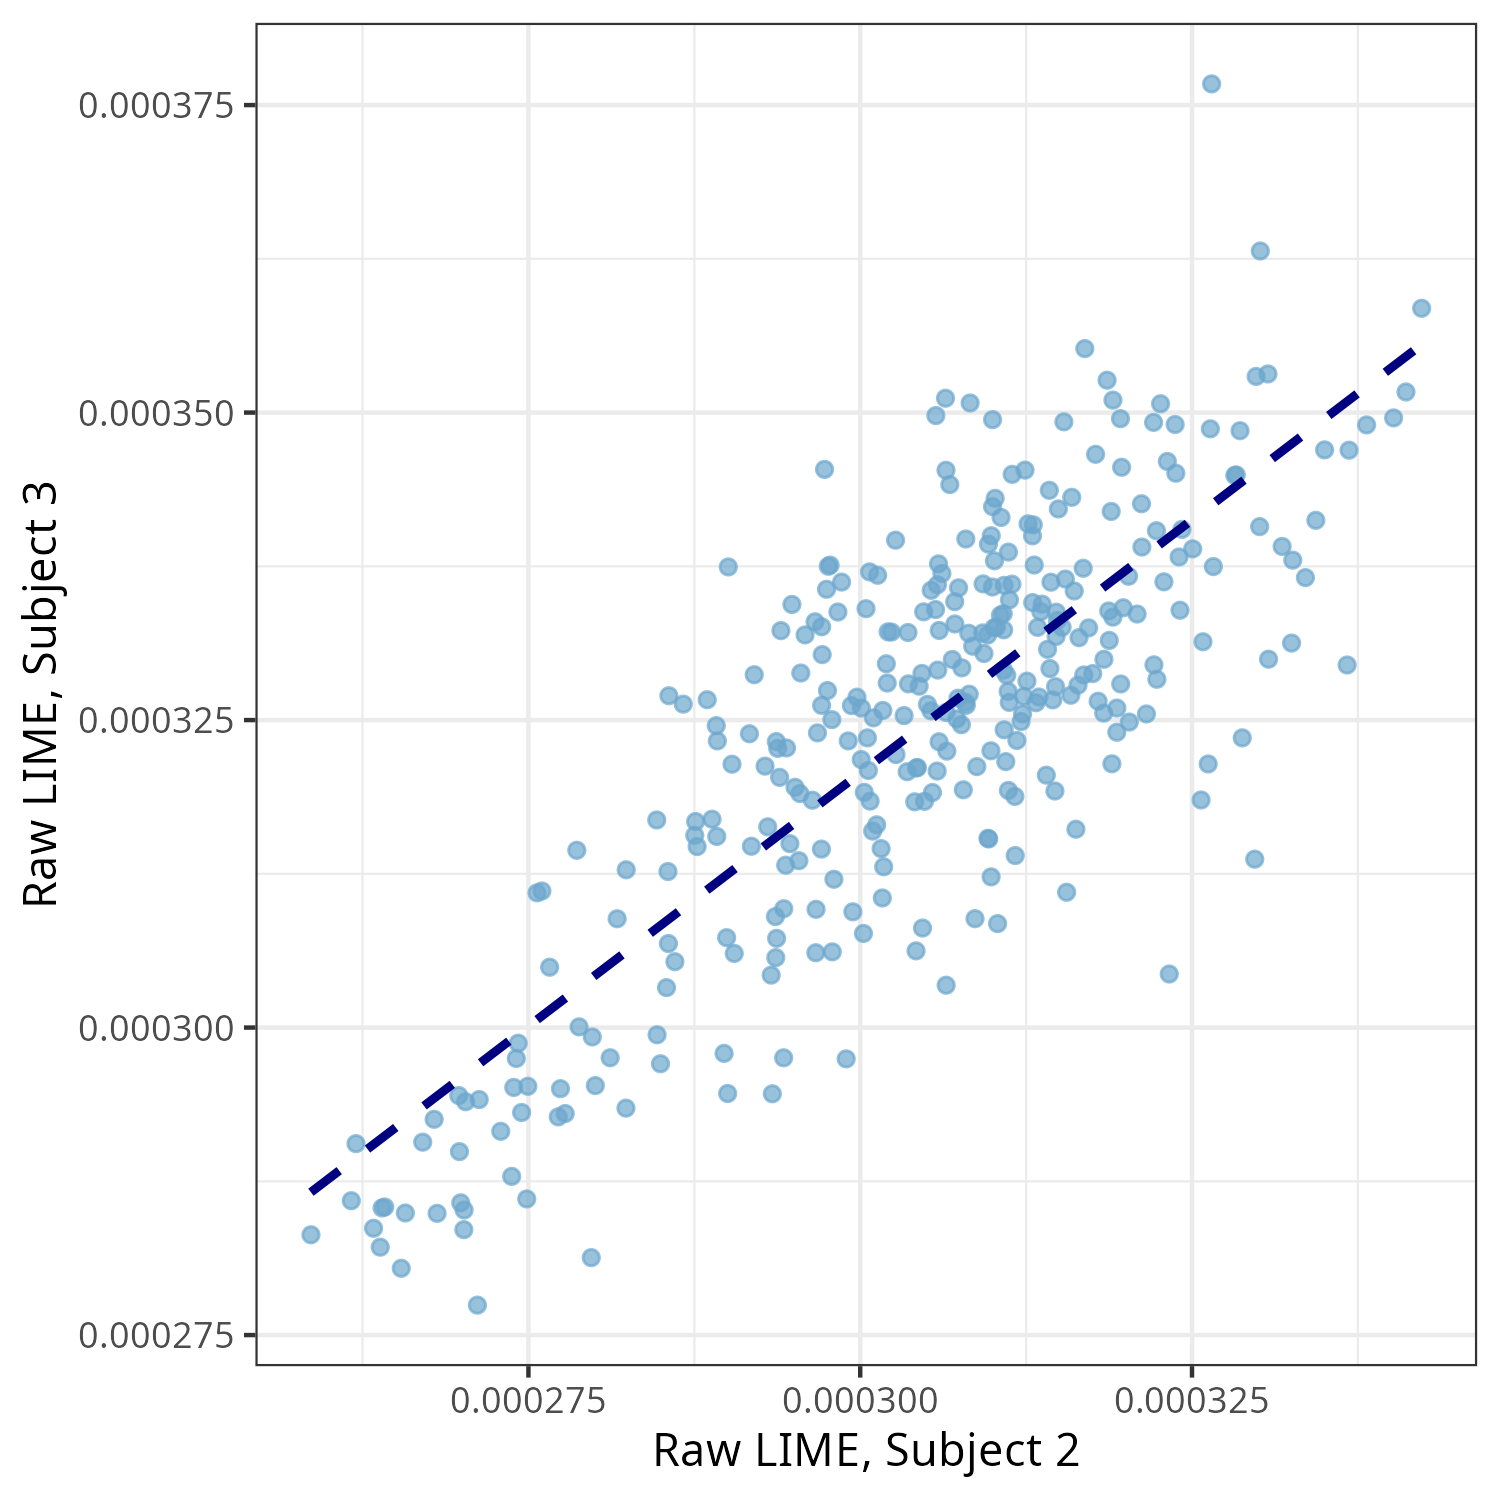
\includegraphics[width=\textwidth]{figs/scatter_buck_lime_raw.png}
        \label{subfig:scatter_buck_lime_raw}
    \end{subfigure}
    \hfill
    \begin{subfigure}[t]{0.22\textwidth}
        \centering
        \caption{LIME Ranks}
        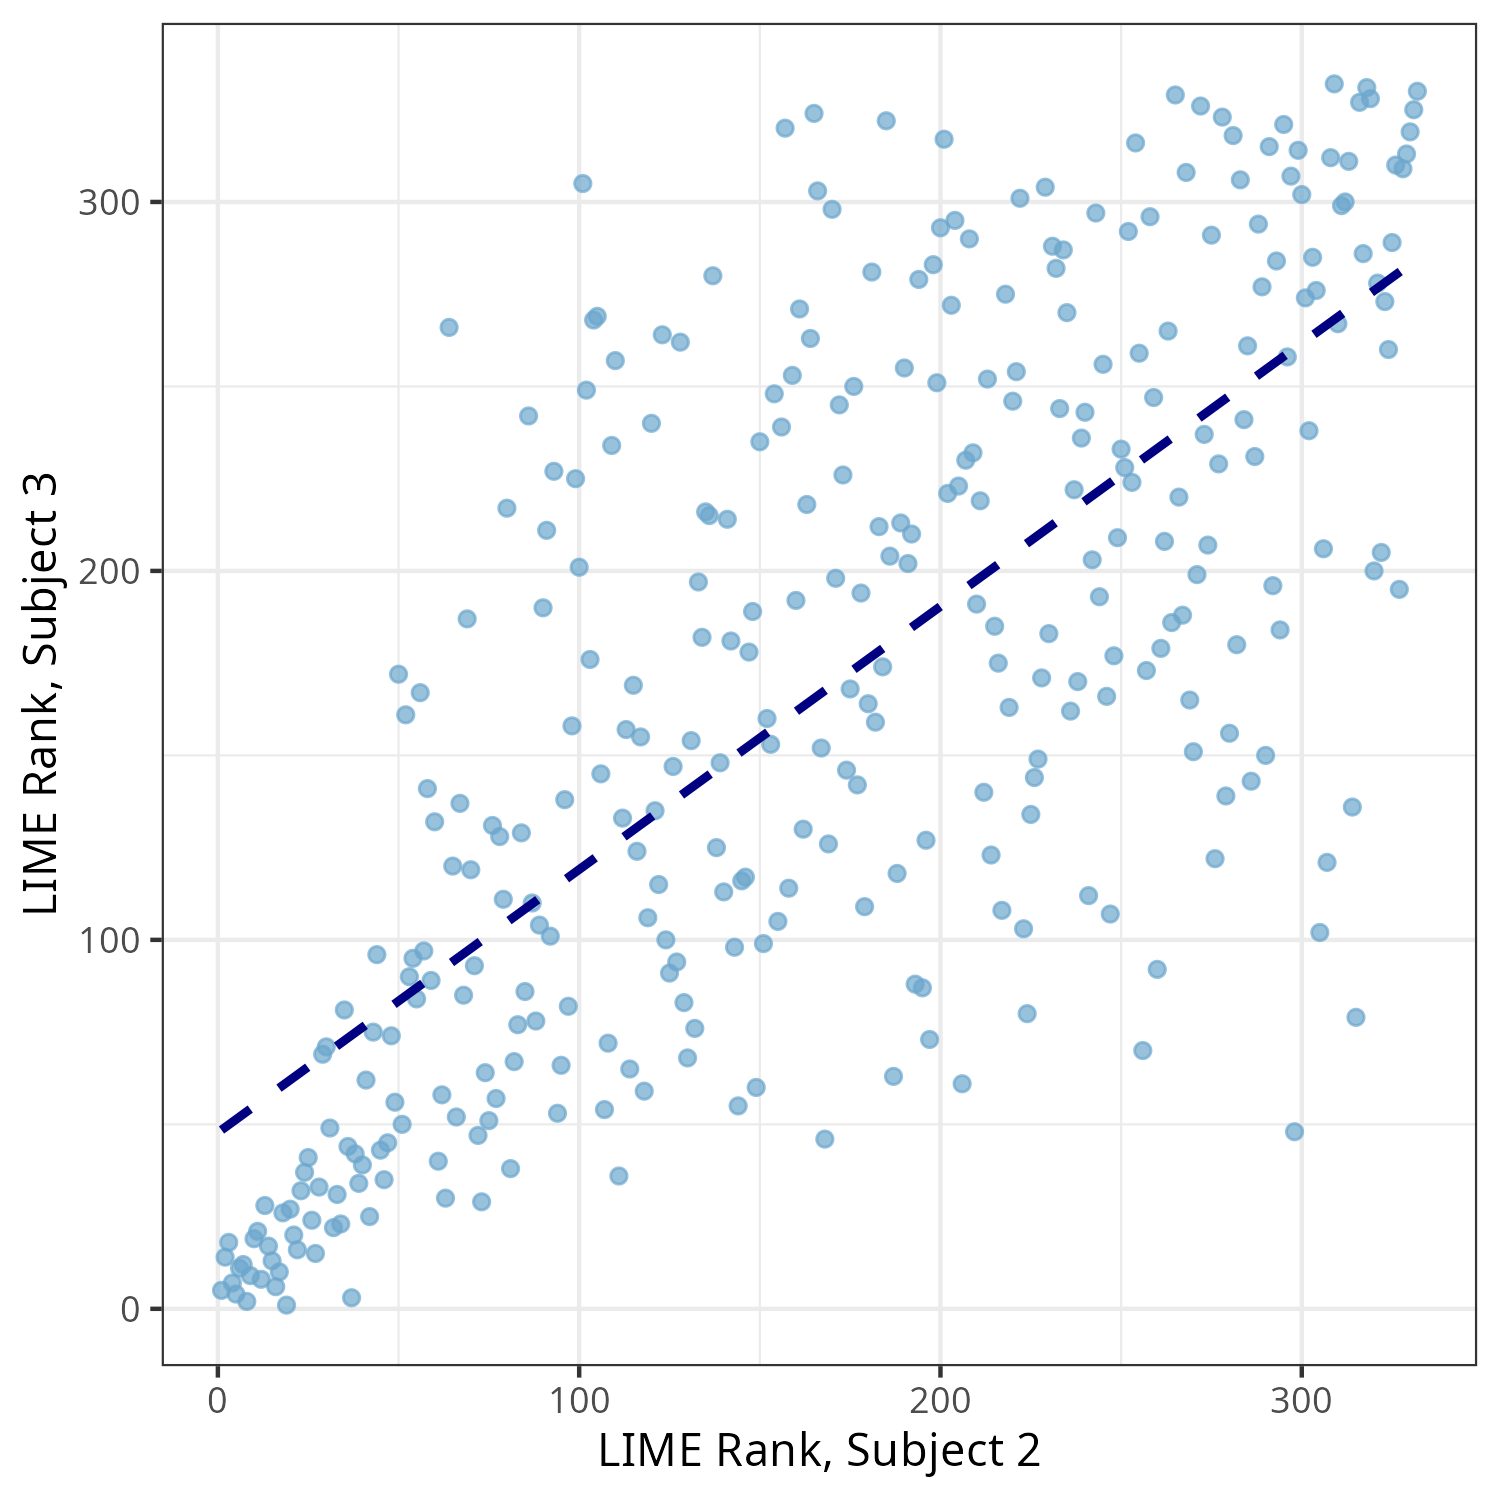
\includegraphics[width=\textwidth]{figs/scatter_buck_lime_rank.png}
        \label{subfig:scatter_buck_lime_rank}
    \end{subfigure}
    \caption{Scatterplots comparing word-level SHAP (red) and LIME (blue) values between Subject 2 and Subject 3. Scores (left) show strong cross-subject agreement, while ranks (right) exhibit greater dispersion—indicating consistency in which words matter, but differences in their relative importance.}
    \label{fig:scatter_buck_1}
\end{figure}

Interestingly, Figure \ref{fig:scatter_buck_2} indicates that the words most highly ranked by SHAP differ substantially from those most highly ranked by LIME. In fact, their word rankings are weakly negatively correlated, implying that SHAP and LIME emphasize different features of the input when assigning importance. This points to complementary but largely divergent interpretations of model behavior by the two methods and suggests instability.

\begin{figure}[ht]
    \centering

    \parbox{\textwidth}{\centering 
        \fontsize{13pt}{13pt}\selectfont \textbf{SHAP vs. LIME: Average Word Rank Comparison}  
        
        {\fontsize{11pt}{13pt}\selectfont Comparing average word ranks across Subject 2 and Subject 3} 
    }
  
    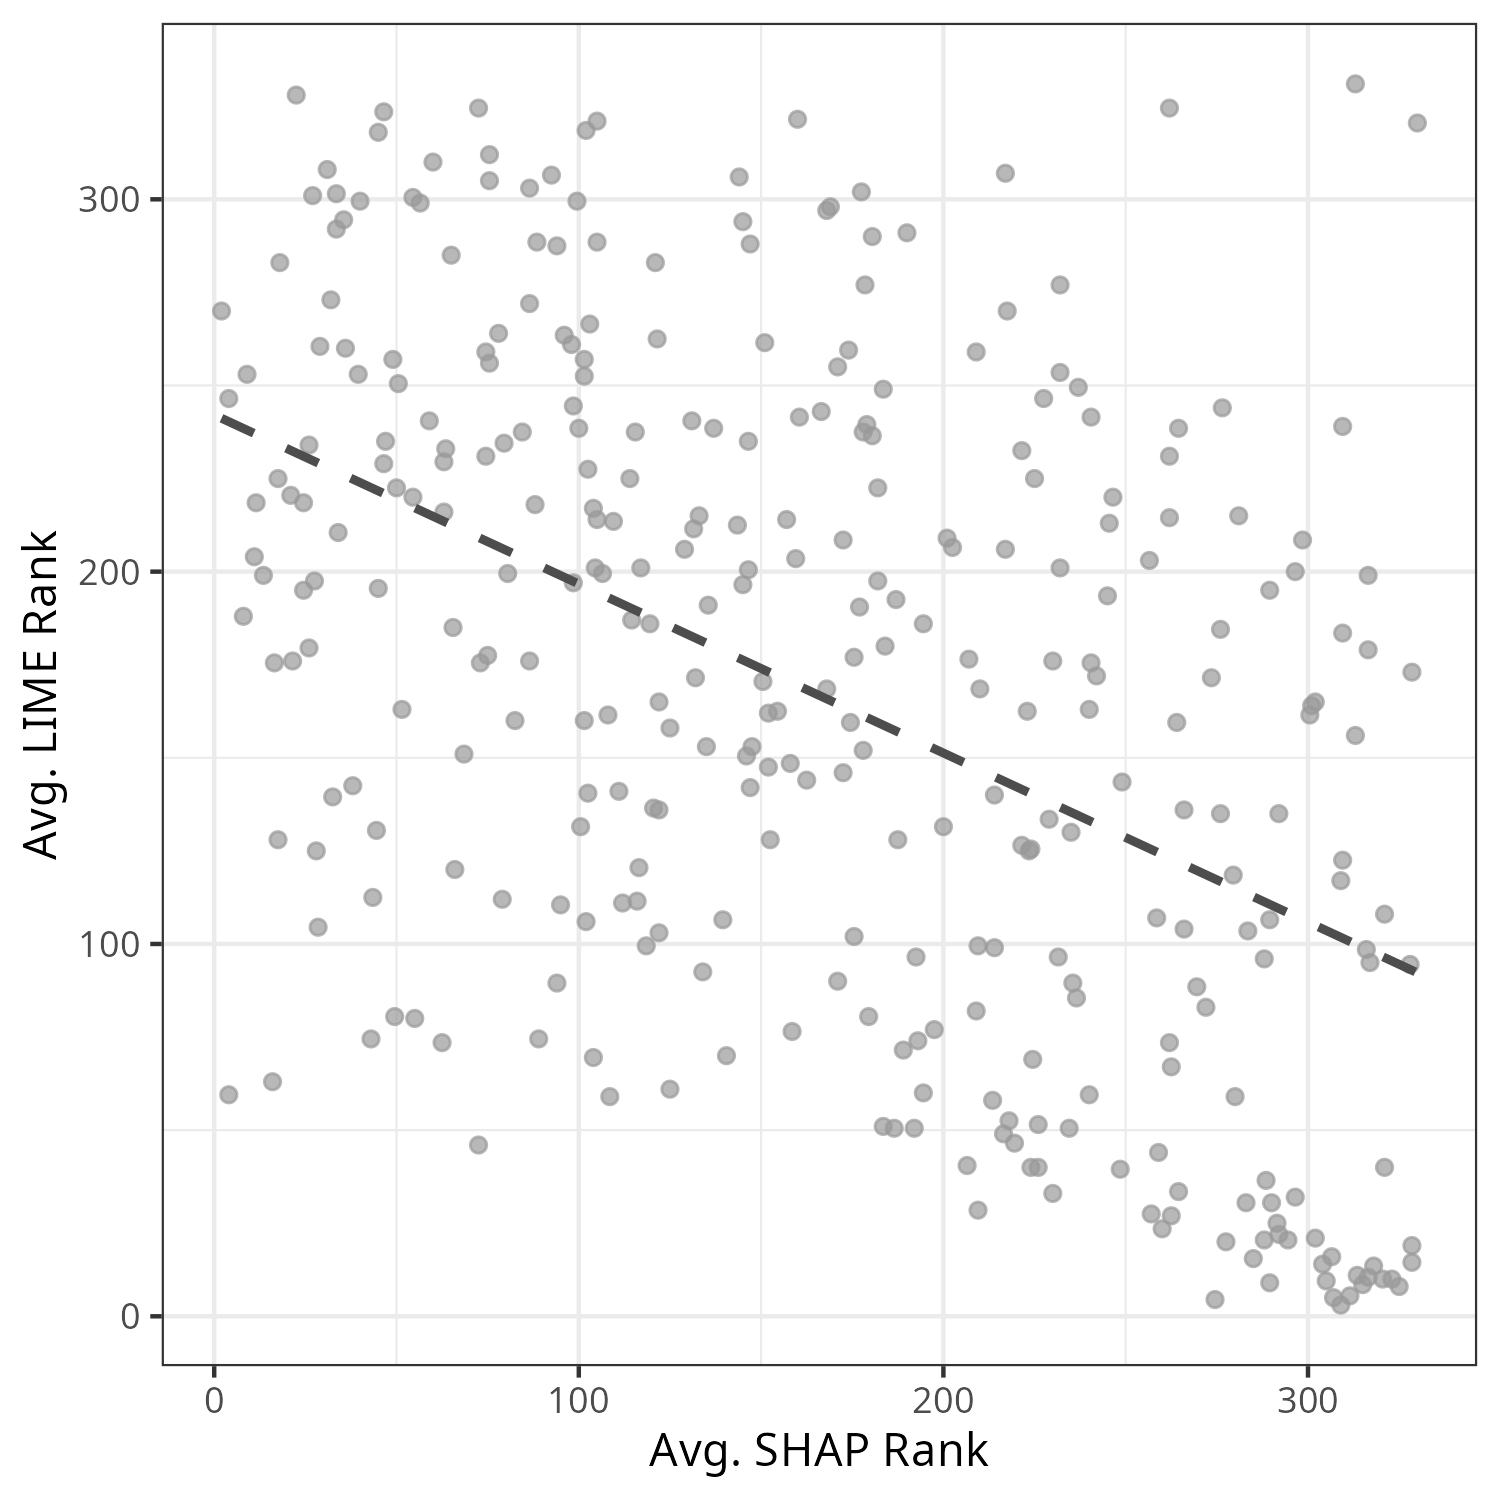
\includegraphics[width=0.35\textwidth]{figs/scatter_buck_rank.png}
    
    \caption{The weak negative correlation $r = -0.35$ between SHAP ranks (x-axis) and LIME ranks (y-axis) suggests that the two methods often prioritize different sets of words, even when averaged across subjects.}
    \label{fig:scatter_buck_2}
\end{figure}


In \texttt{buck}, SHAP tends to highlight:
\begin{itemize}
	\item \textbf{Emotional experiences} (e.g., "to eat from this spread", "no one had ever asked me what i want")
	\item \textbf{Prison dynamics} (e.g., "prison", "walk the one gate after another", "hundred guys waiting", "[out] of prison they know you on parole")
	\item \textbf{Identity markers} (e.g., "know this ink work this is prison ink", "now i speak a lot of different gangster languages", "understand blood i even speak a little")
	\item \textbf{Transitional phrases} (e.g., "so", "because for the past ten years", "and leave out of here")
\end{itemize}


Meanwhile, LIME tends to highlight:
\begin{itemize}
	\item \textbf{Temporal markers} (e.g., "after twenty six years", "corridor for the last time", "through that last gate")
	\item \textbf{Quantitative details} (e.g., "thirty seven eighty seven five report", "with two hundred dollars in it", "no more than eight feet away")
	\item \textbf{Action sequences} (e.g., "they load us on a van", "i get to r and r", "washing dishes my wife says")
\end{itemize}

Curiously, words identified by both methods almost exclusively involve \textbf{interactions with the speaker's wife} (e.g., "gave her a quick kiss whispered in", "call out to my wife i said hey babe", "i could see her she was snapping pictures", "and he tells my wife wait").

This pattern suggests that these two methods can provide complementary insights about which textual features drive fMRI responses: SHAP may better capture emotional and thematic elements, while LIME may be more effective at identifying sequentially important narrative details. For a more comprehensive list of words identified by each method, see Appendix \ref{sec:buck_text}.

\begin{figure}[ht]
    \centering

    \parbox{\textwidth}{\centering 
        \fontsize{13pt}{13pt}\selectfont \textbf{Voxelwise Consistency of SHAP and LIME Word Ranks}  
        
        {\fontsize{11pt}{13pt}\selectfont Distribution of word rankings across individual voxels and subject-score combinations} 
    }
    
    \begin{subfigure}[t]{0.35\textwidth}
        \centering
        \caption{Voxelwise Rank Heatmap}
        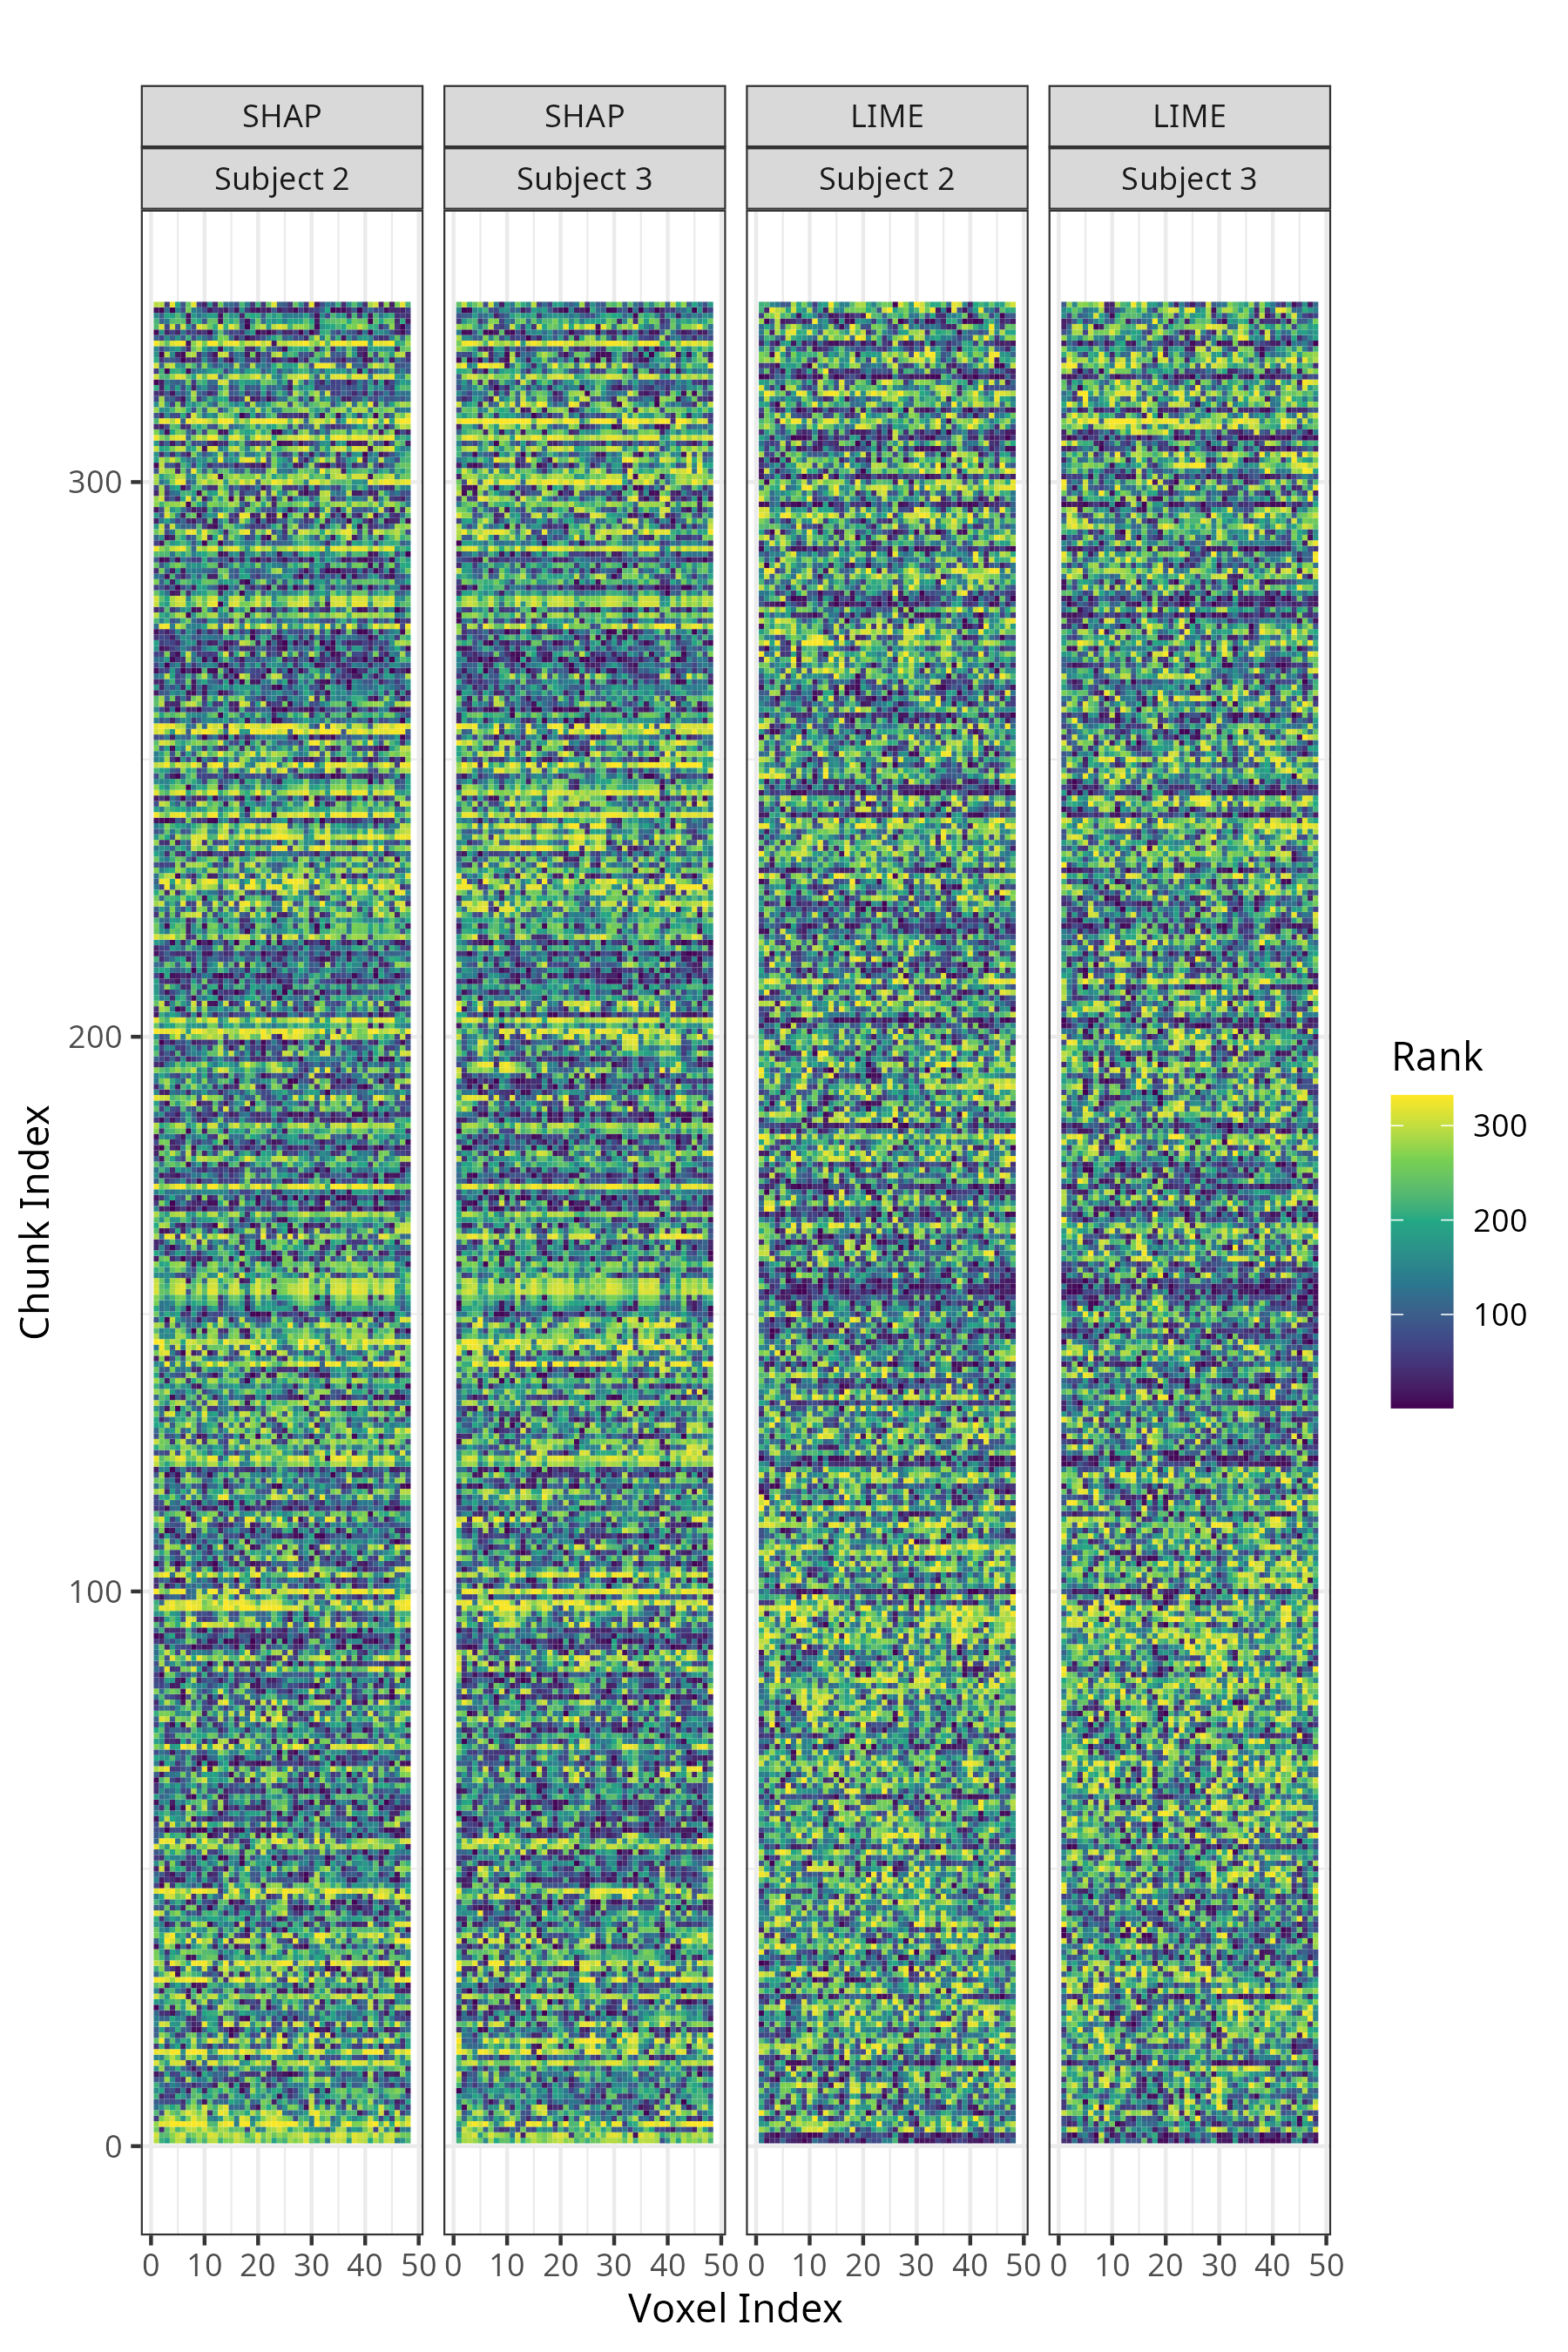
\includegraphics[width=\textwidth]{figs/heatmap_buck.png}
        \label{subfig:heatmap_buck}
    \end{subfigure}
    \hfill
    \begin{subfigure}[t]{0.35\textwidth}
        \centering
        \caption{Interquartile Range of Word Ranks}
        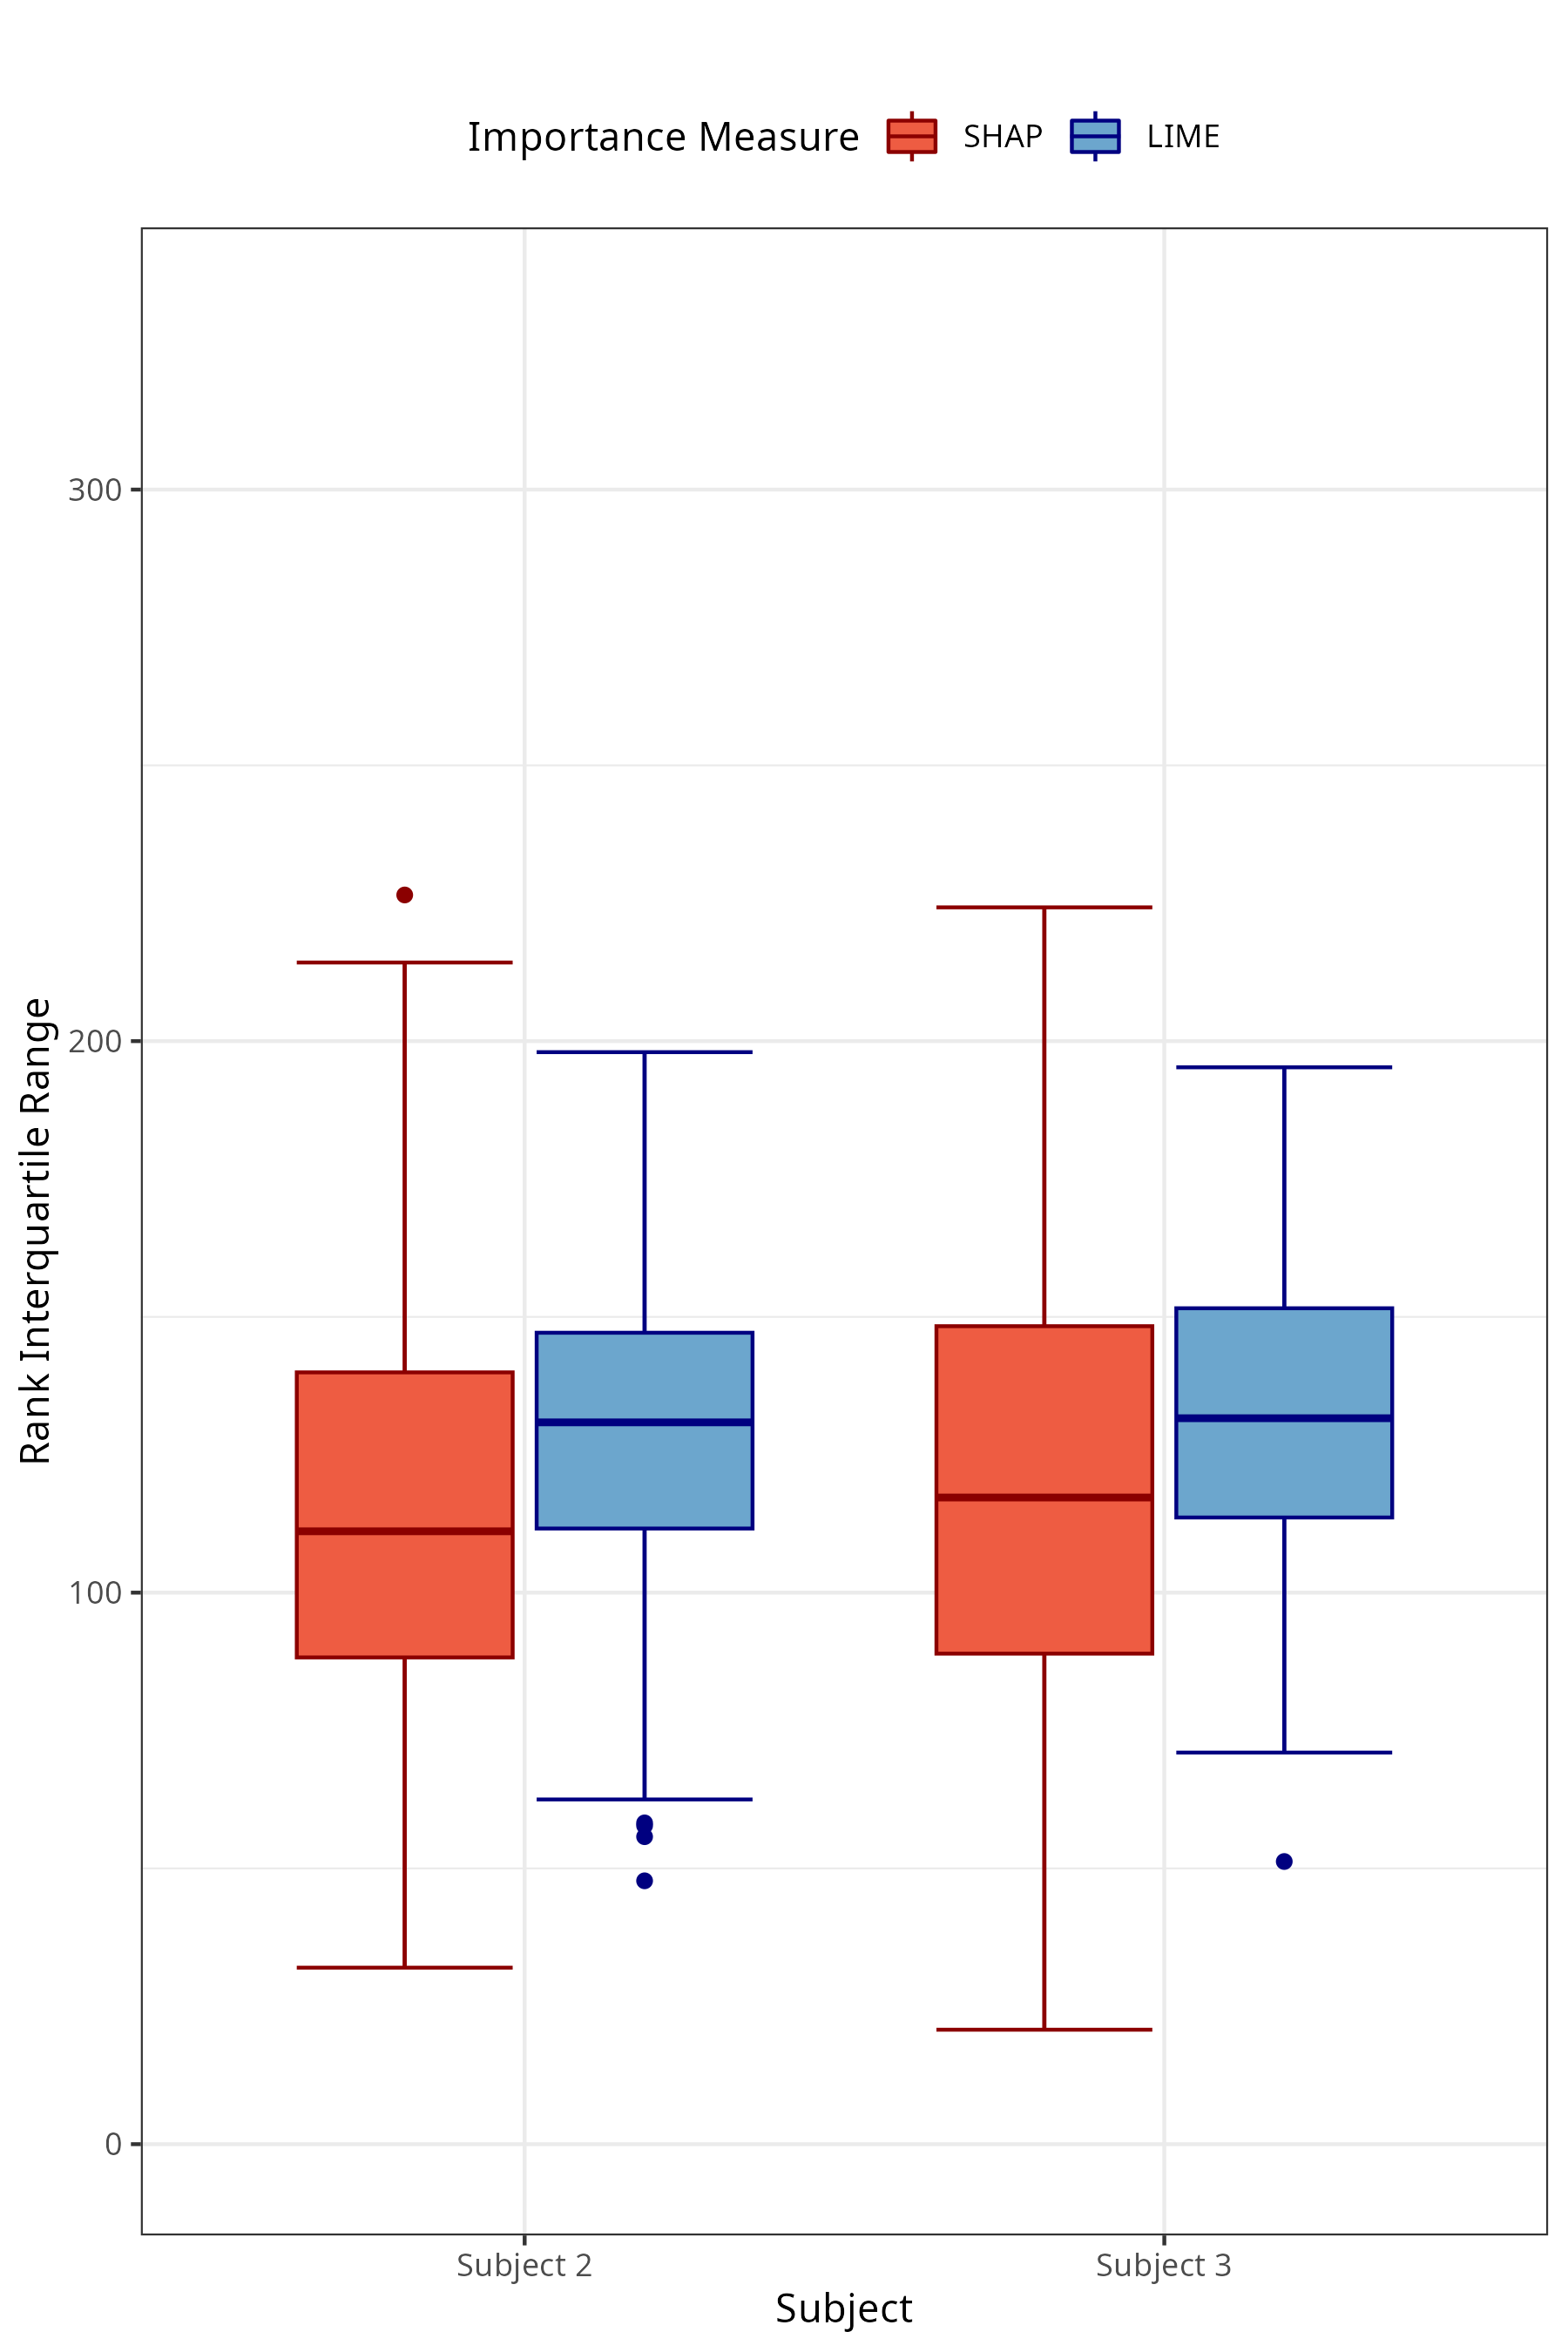
\includegraphics[width=\textwidth]{figs/boxplot_buck.png}
        \label{subfig:boxplot_buck}
    \end{subfigure}
    \caption{Word ranks assigned by individual voxels show a high degree of consistency within and across subjects. The heatmap (left) displays voxelwise rankings for 332 word chunks, revealing horizontal banding patterns that reflect agreement in word importance. The boxplot (right) summarizes the spread of these ranks within chunks. For the average word, the IQR spans only ${\sim}125$ ranks, suggesting relatively stable importance scores across voxels.}
    \label{fig:buck_voxelwise}
\end{figure}

\newpage

Regarding differences across voxels, Figure \ref{fig:buck_voxelwise} reveals visible horizontal banding in the heatmaps for both SHAP and LIME, indicating that word rankings are relatively consistent across voxels within and between subjects. The accompanying boxplot shows that SHAP produces slightly lower median IQRs for word ranks across voxels, suggesting less variability and lower voxel sensitivity for the average word. Conversely, LIME exhibits a tighter distribution of IQR values, indicating that while its average variability may be higher, the spread among the least consistently ranked words is smaller.


\subsection{Test Story 2: \texttt{lawsthatchokecreativity}}

As shown in Figure \ref{fig:scatter_laws_1}, the word rankings produced by SHAP and LIME for \texttt{lawsthatchokecreativity} are fairly consistent between Subject 2 and Subject 3, although the correlation is weaker than that observed for the raw attribution scores. This suggests that both SHAP- and LIME-based word importances are relatively stable across listeners to this story.


\begin{figure}[ht]
    \centering

    \parbox{\textwidth}{\centering 
        \fontsize{13pt}{13pt}\selectfont \textbf{Cross-Subject Consistency in Word Importance}  
        
        {\fontsize{11pt}{13pt}\selectfont Comparing SHAP and LIME scores and ranks between Subject 2 and Subject 3} 
    }
    
    \begin{subfigure}[t]{0.22\textwidth}
        \centering
        \caption{SHAP Scores}
        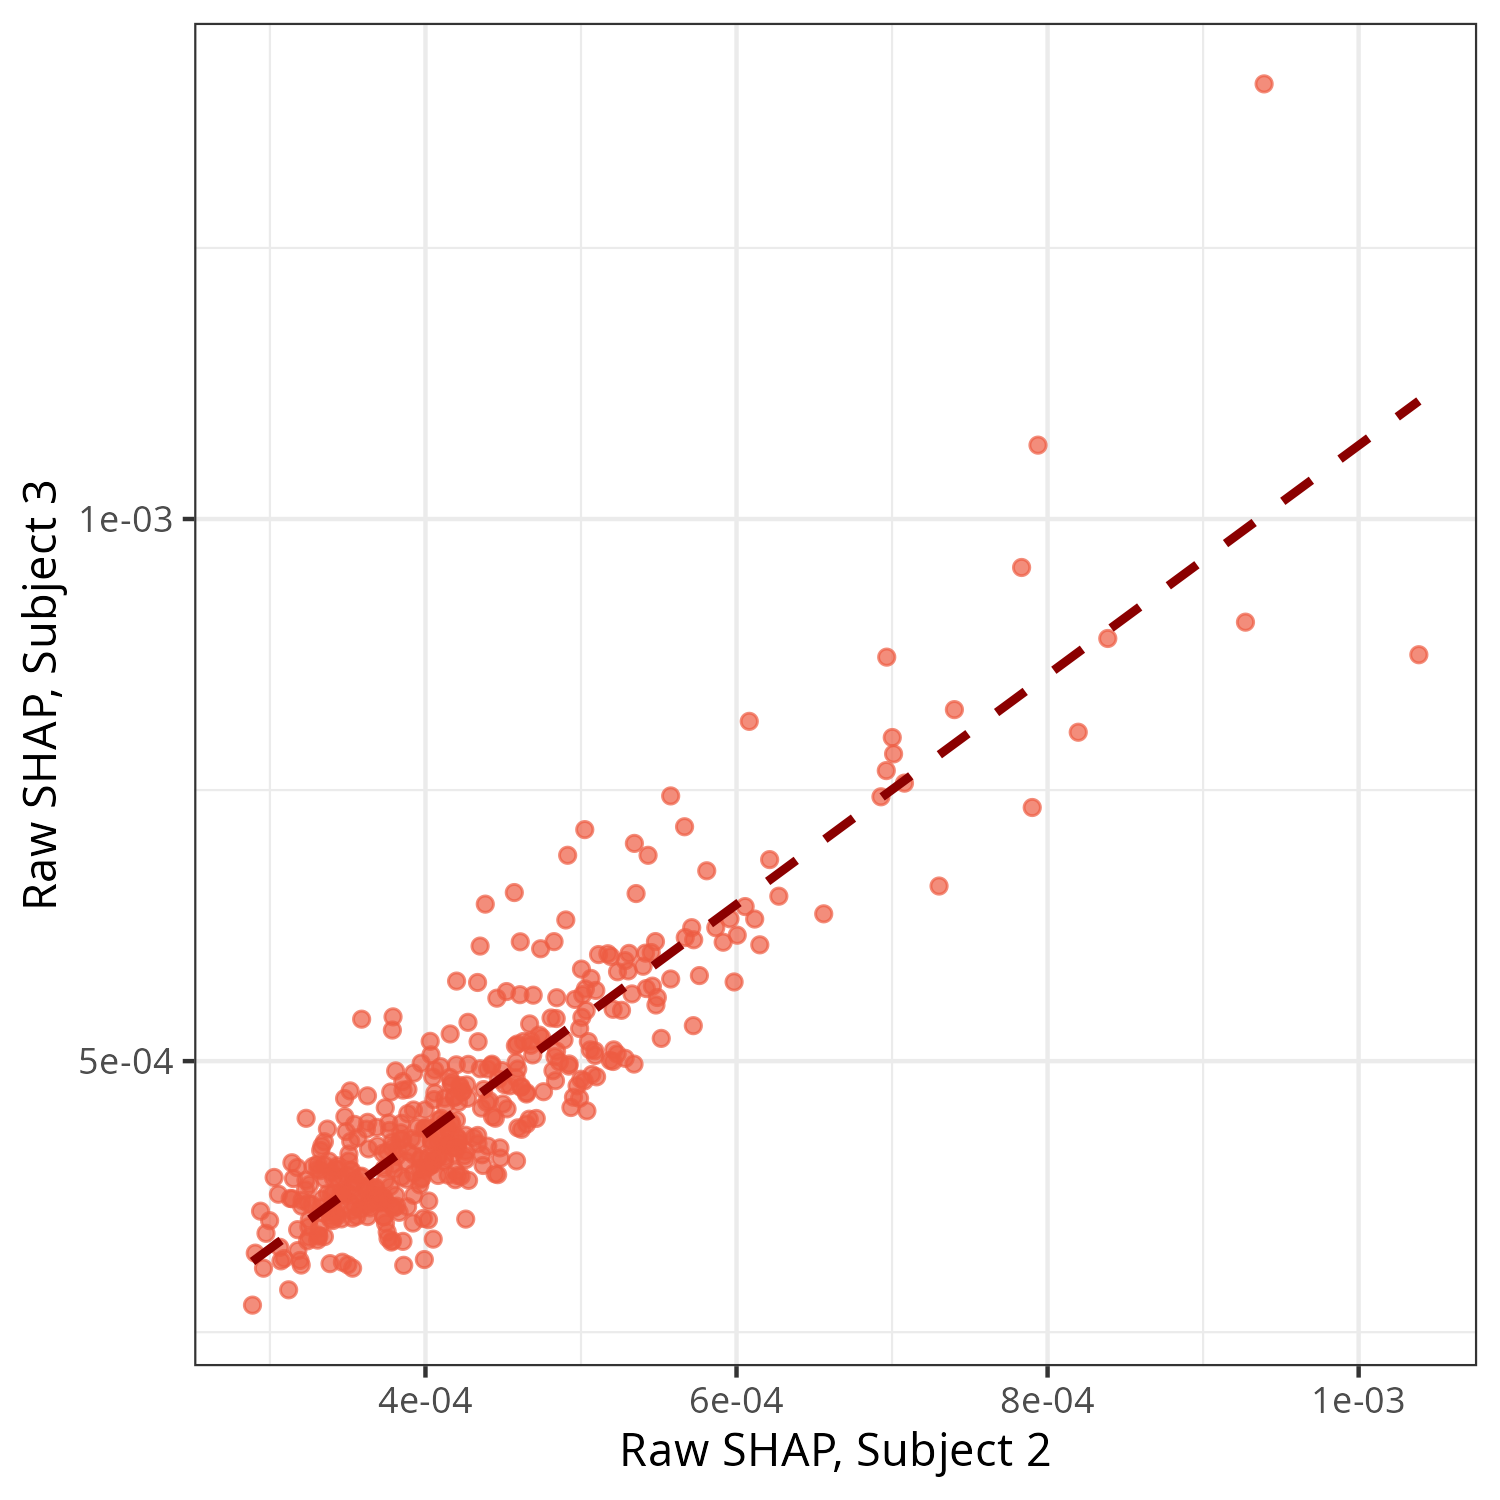
\includegraphics[width=\textwidth]{figs/scatter_laws_shap_raw.png}
        \label{subfig:scatter_laws_shap_raw}
    \end{subfigure}
    \hfill
    \begin{subfigure}[t]{0.22\textwidth}
        \centering
        \caption{SHAP Ranks}
        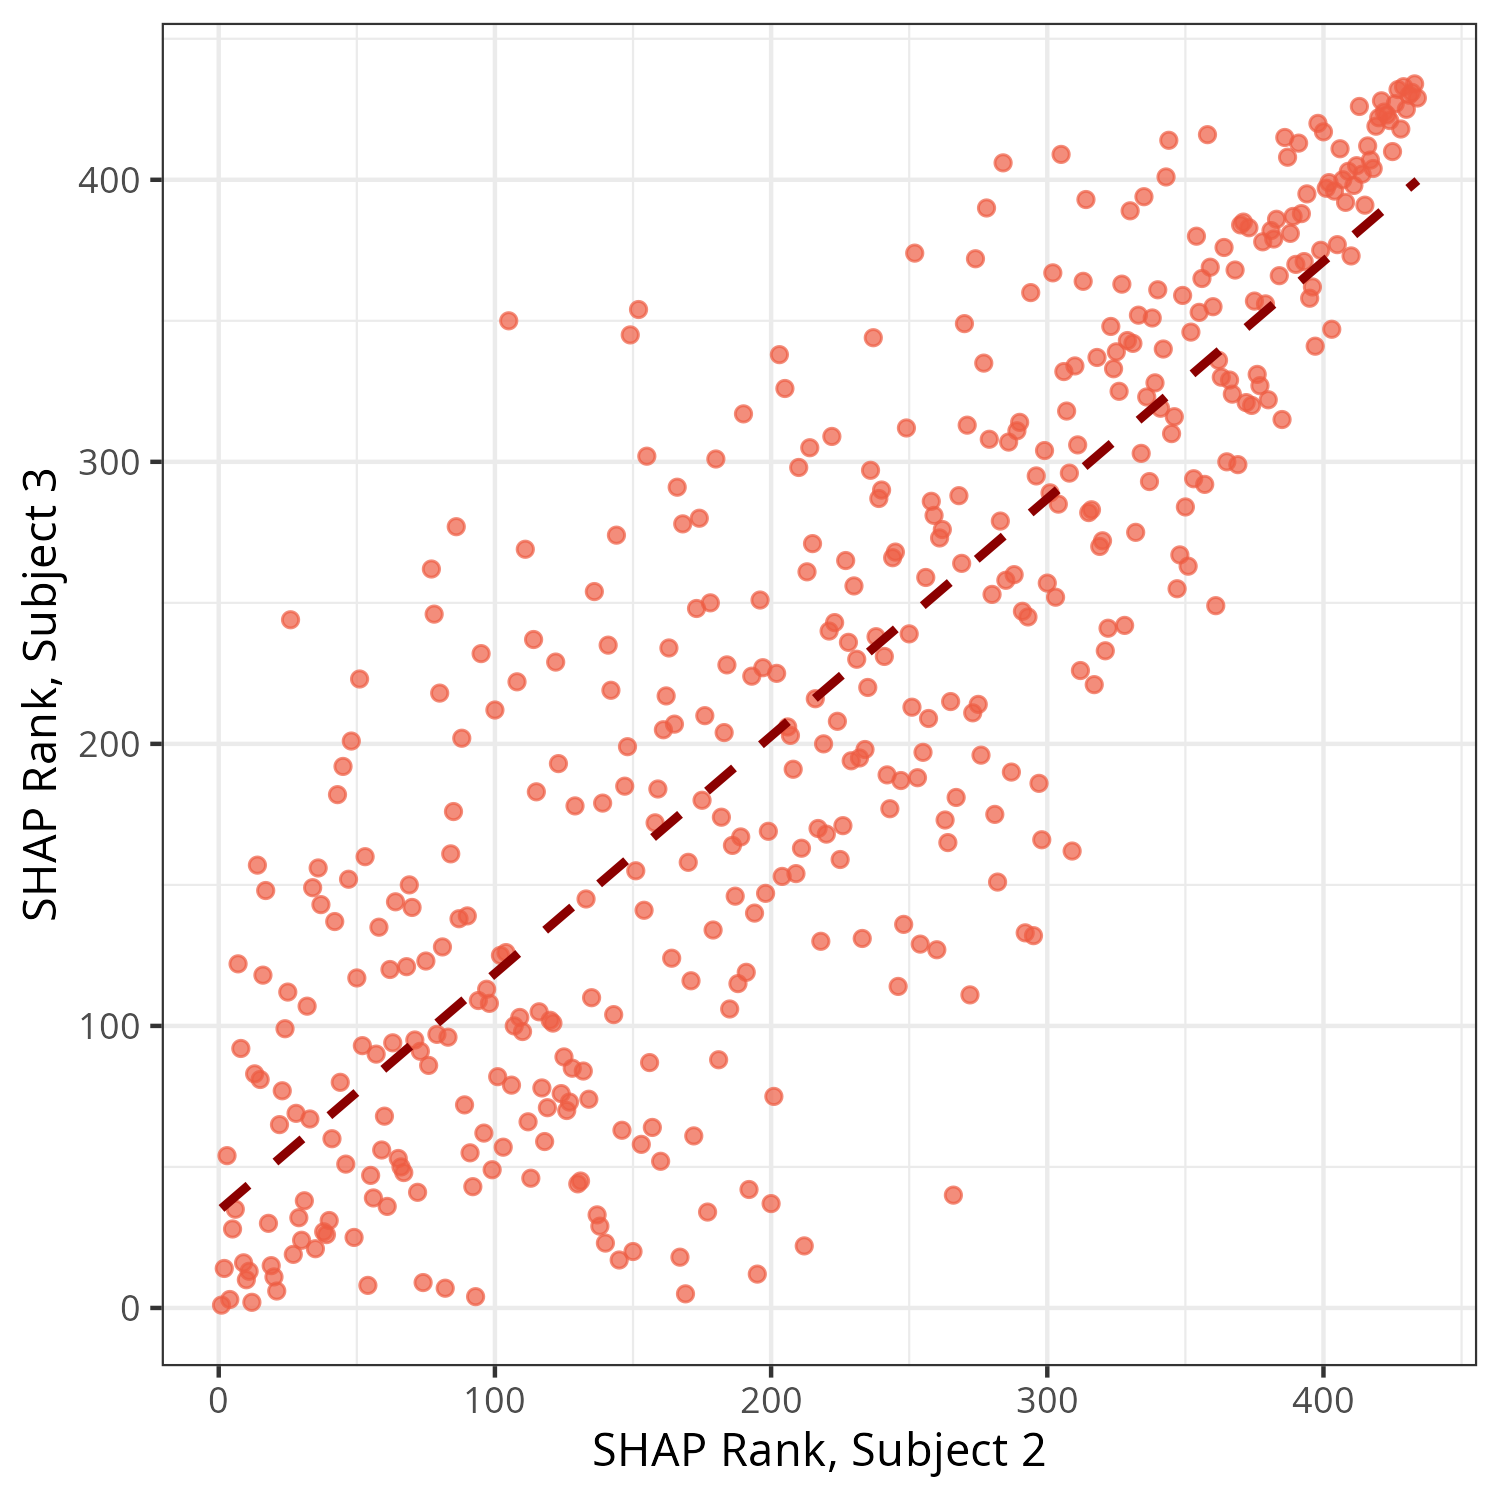
\includegraphics[width=\textwidth]{figs/scatter_laws_shap_rank.png}
        \label{subfig:scatter_laws_shap_rank}
    \end{subfigure}
    \hfill
    \begin{subfigure}[t]{0.22\textwidth}
        \centering
        \caption{LIME Scores}
        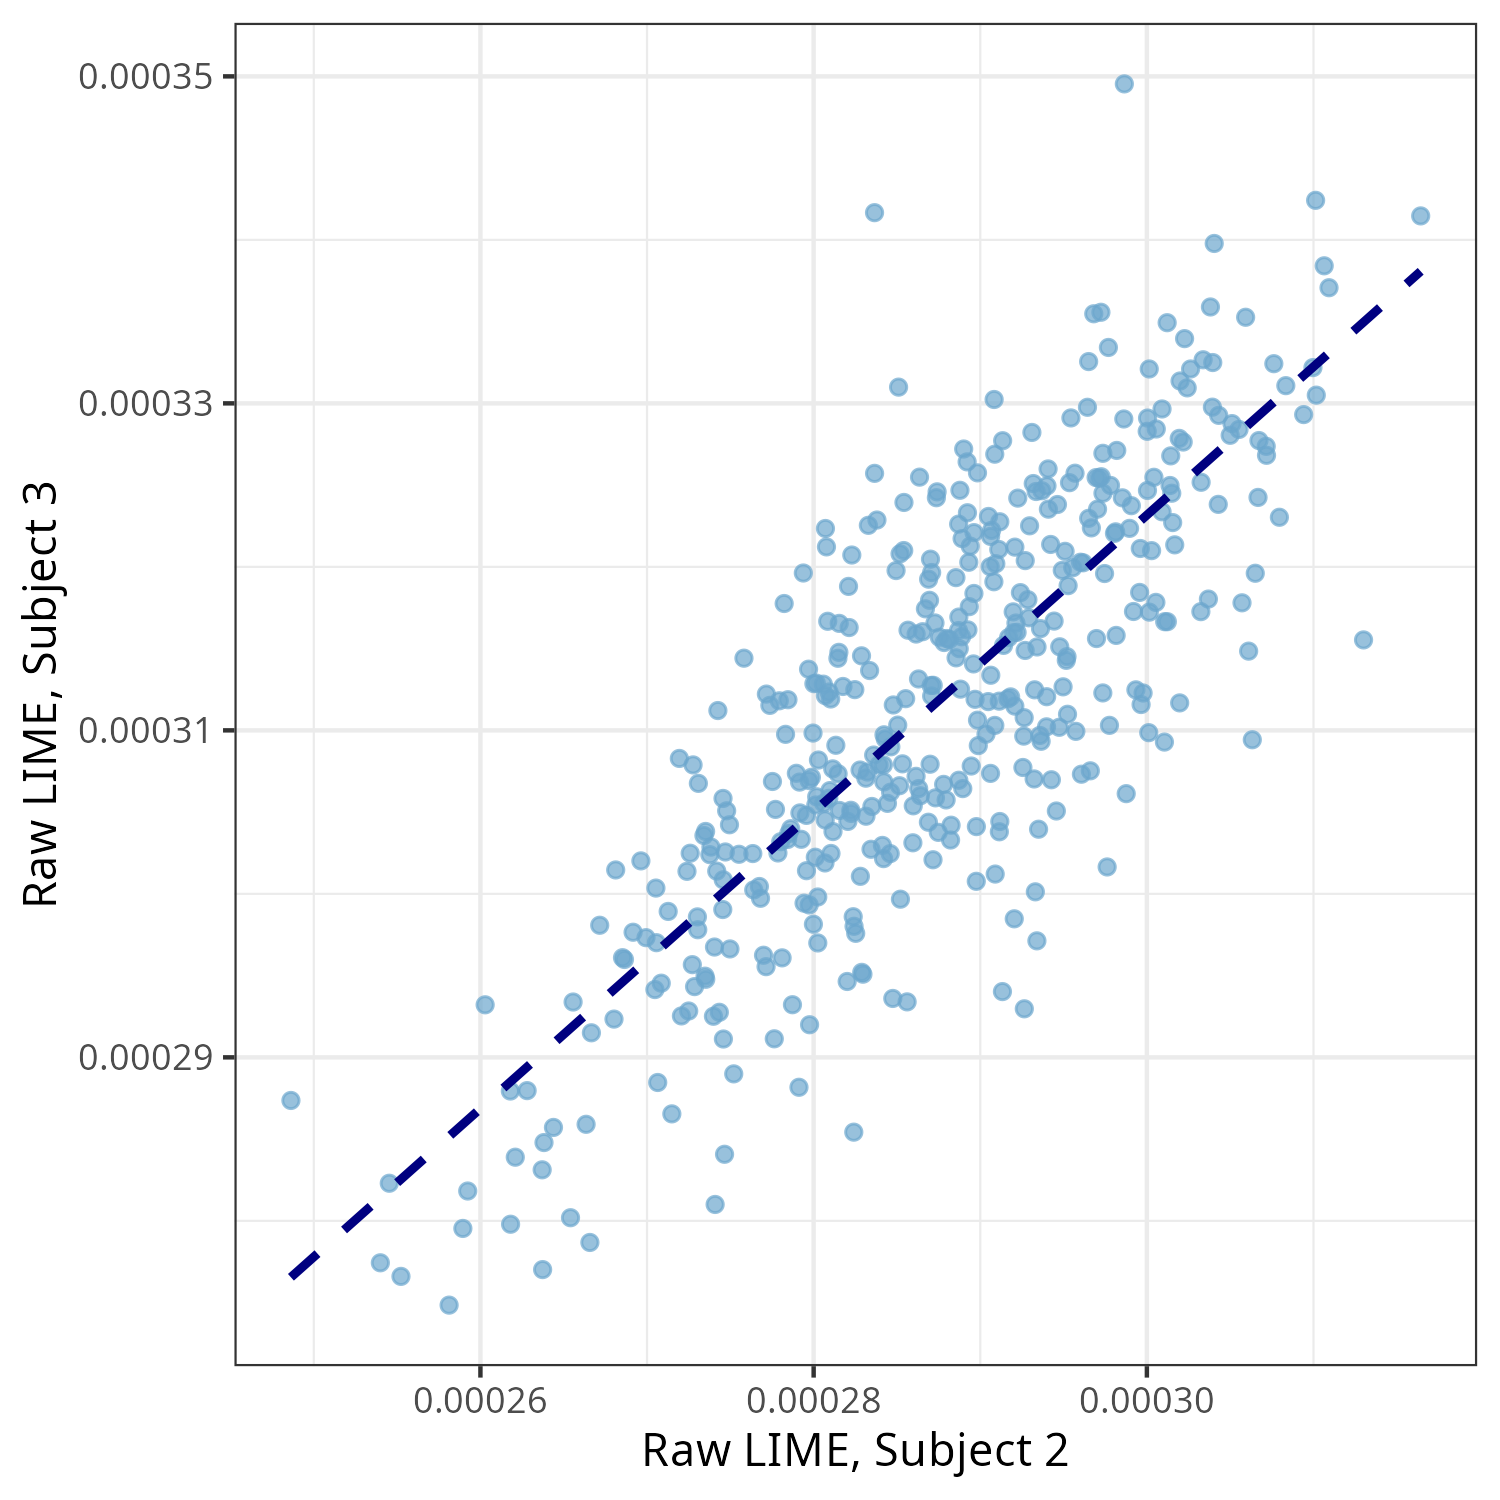
\includegraphics[width=\textwidth]{figs/scatter_laws_lime_raw.png}
        \label{subfig:scatter_laws_lime_raw}
    \end{subfigure}
    \hfill
    \begin{subfigure}[t]{0.22\textwidth}
        \centering
        \caption{LIME Ranks}
        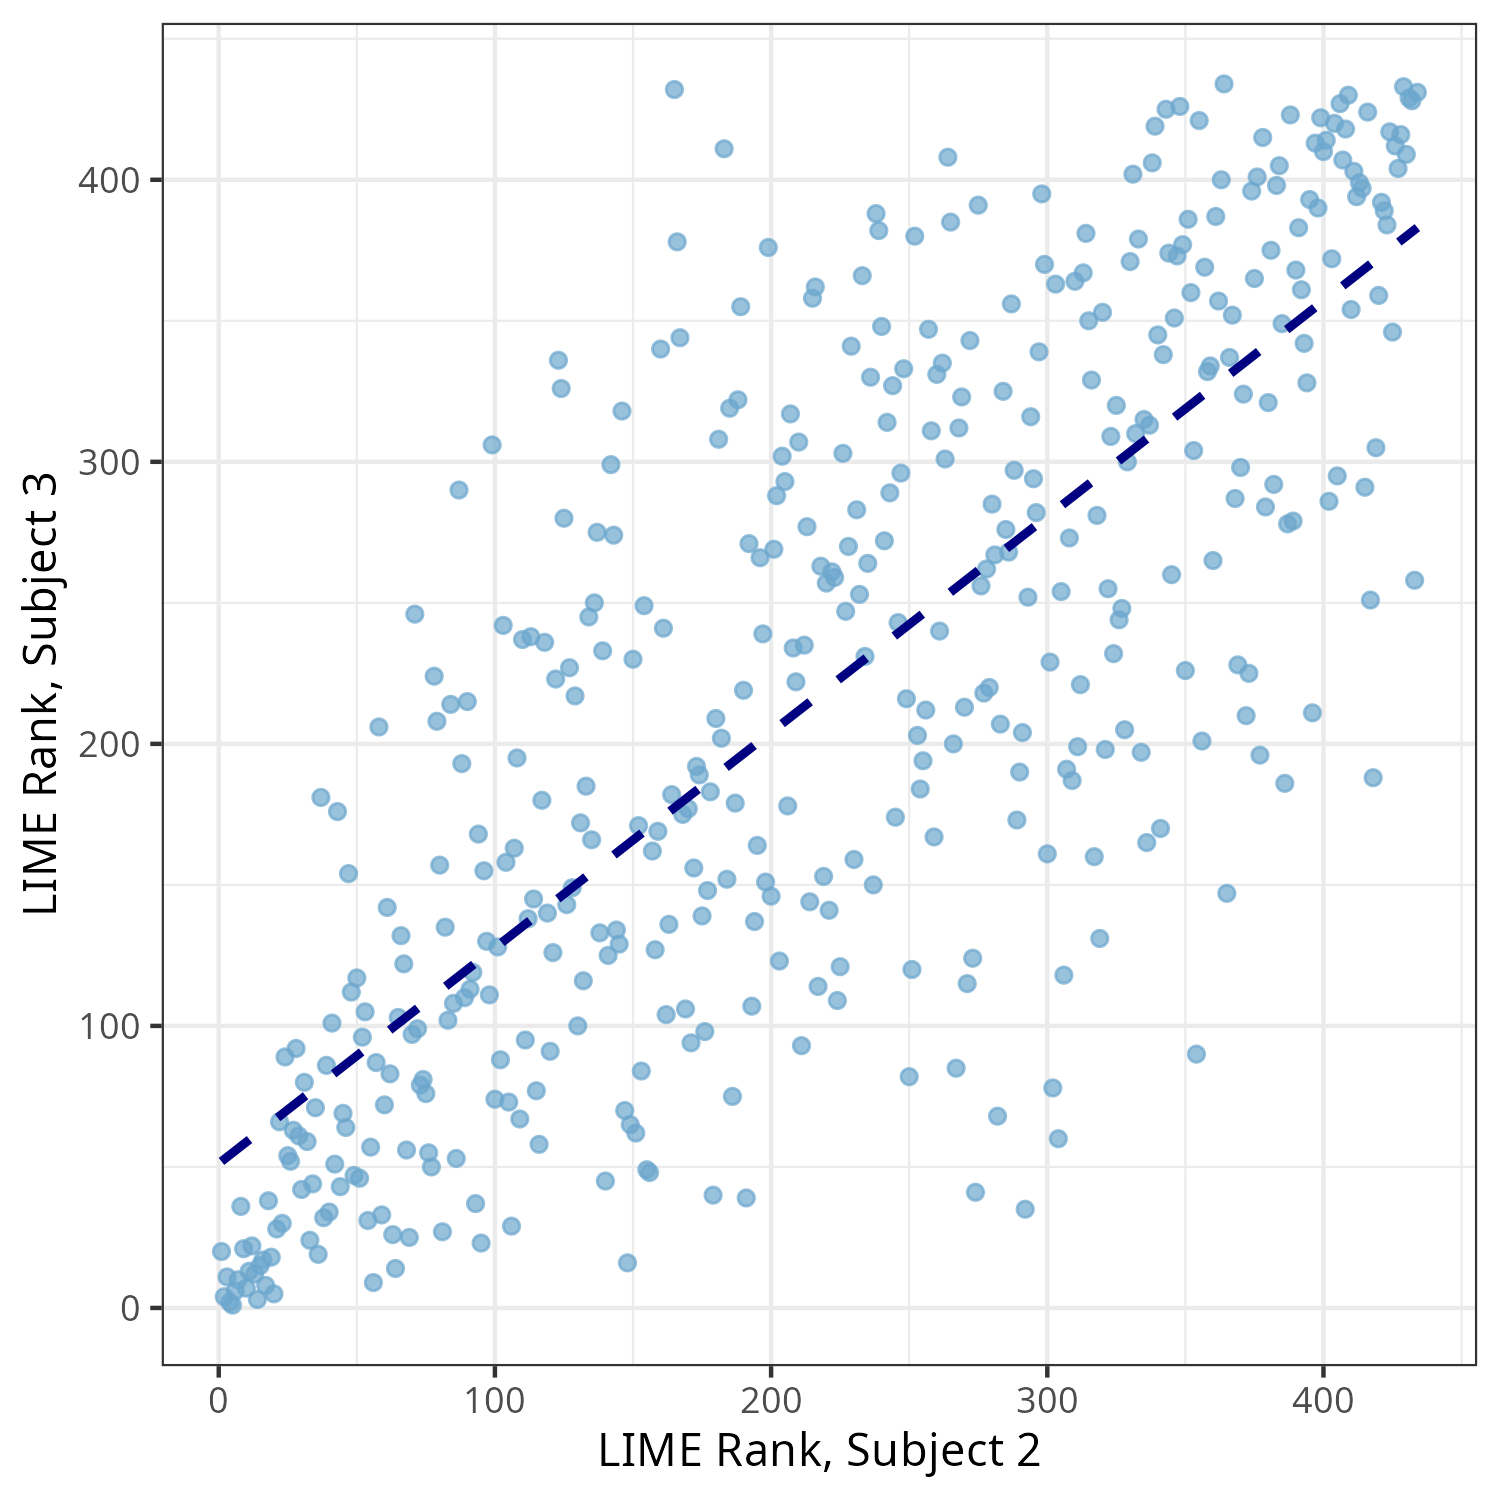
\includegraphics[width=\textwidth]{figs/scatter_laws_lime_rank.png}
        \label{subfig:scatter_laws_lime_rank}
    \end{subfigure}
    \caption{Scatterplots comparing word-level SHAP (red) and LIME (blue) values between Subject 2 and Subject 3. Scores (left) show strong cross-subject agreement, while ranks (right) exhibit greater dispersion—indicating consistency in which words matter, but differences in their relative importance.}
    \label{fig:scatter_laws_1}
\end{figure}


Interestingly, Figure \ref{fig:scatter_laws_2} indicates that the words most highly ranked by SHAP differ substantially from those most highly ranked by LIME. In fact, their word rankings are weakly negatively correlated, implying that SHAP and LIME emphasize different features of the input when assigning importance. This points to complementary but largely divergent interpretations of model behavior by the two methods.


\begin{figure}[ht]
    \centering

    \parbox{\textwidth}{\centering 
        \fontsize{13pt}{13pt}\selectfont \textbf{SHAP vs. LIME: Average Word Rank Comparison}  
        
        {\fontsize{11pt}{13pt}\selectfont Comparing average word ranks across Subject 2 and Subject 3} 
    }
  
    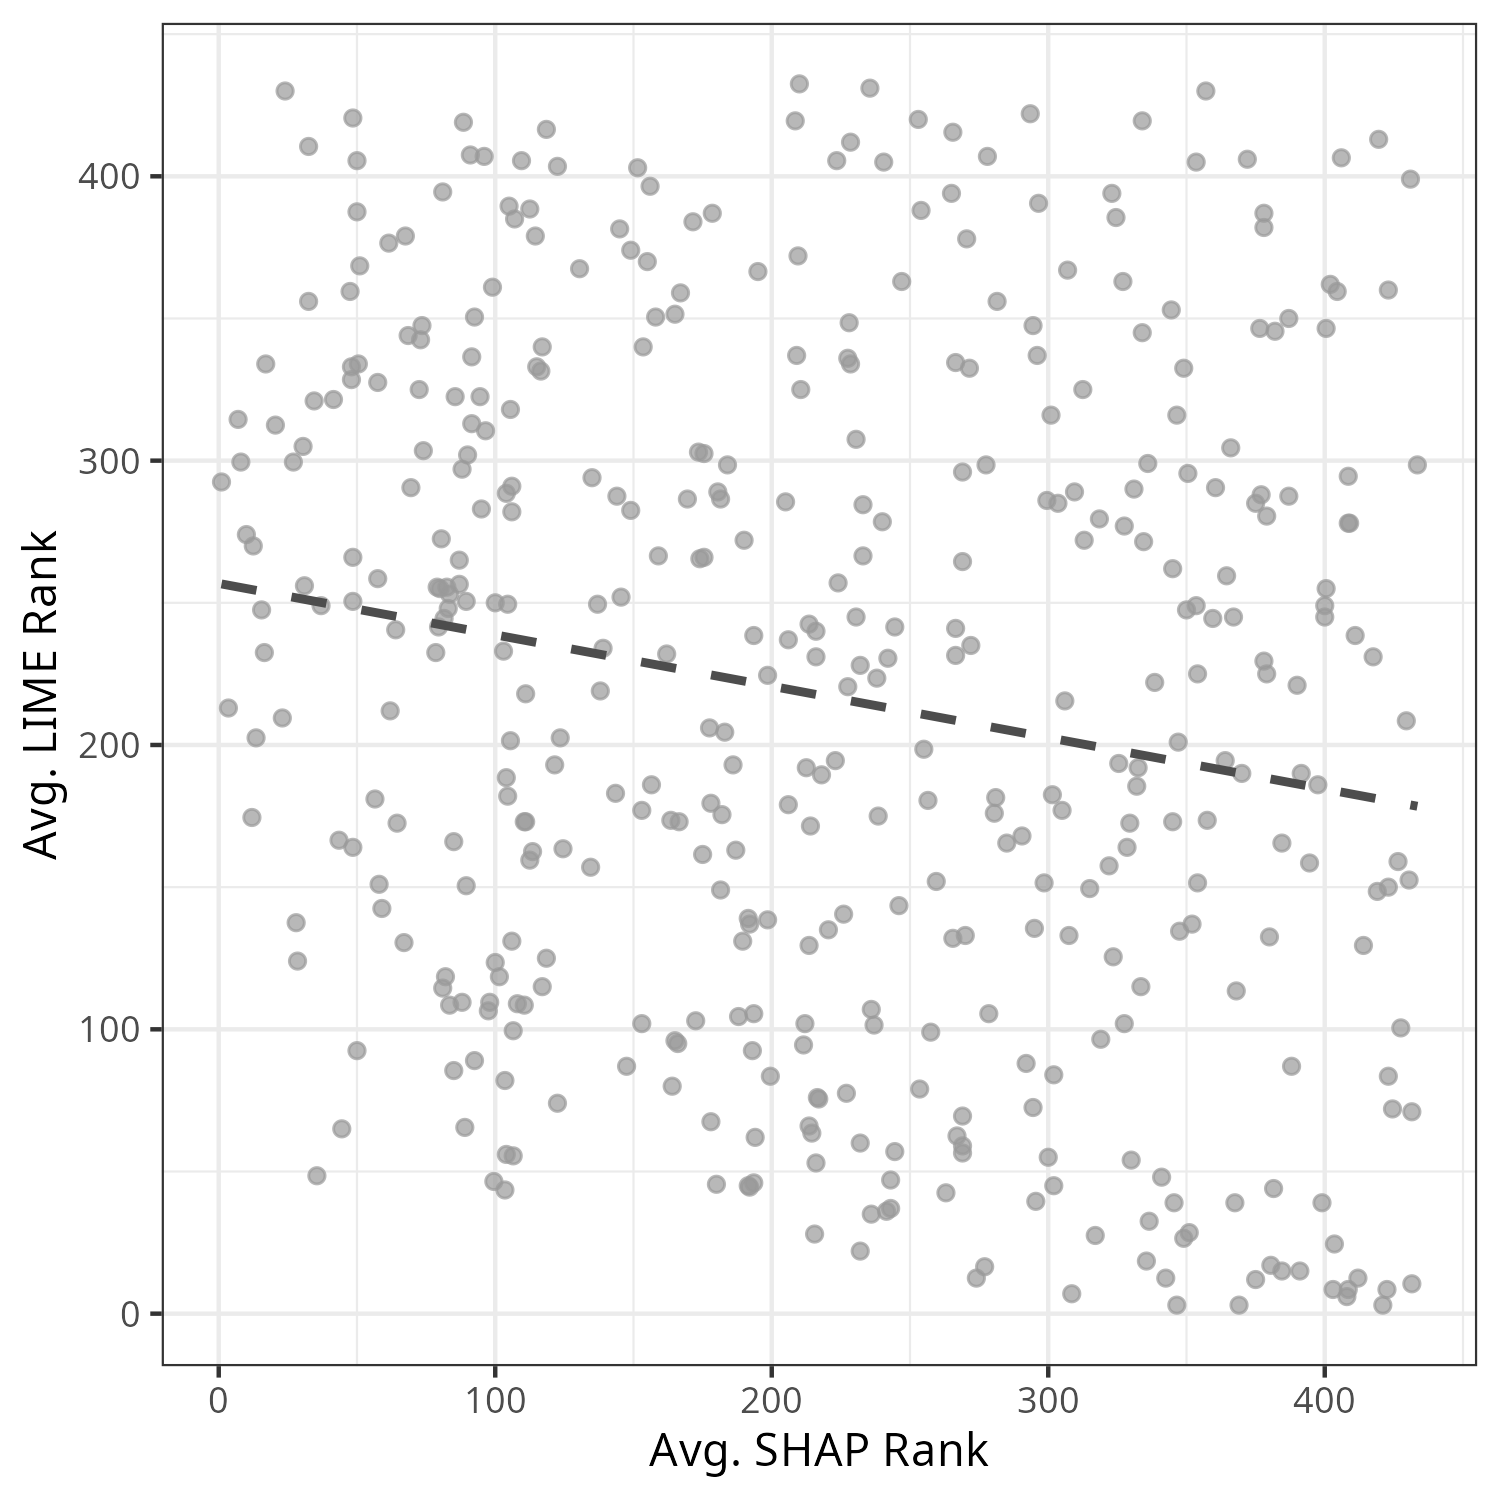
\includegraphics[width=0.3\textwidth]{figs/scatter_laws_rank.png}
    
    \caption{The weak negative correlation $r = -0.12$ between SHAP ranks (x-axis) and LIME ranks (y-axis) suggests that the two methods often prioritize different sets of words, even when averaged across subjects.}
    \label{fig:scatter_laws_2}
\end{figure}

\newpage


In \texttt{lawsthatchokecreativity}, SHAP tends to highlight:
\begin{itemize}
    \item \textbf{Concrete entities and specific references} (e.g., "john philip sousa", "united states capitol", "four hundred and forty eight percent", "supreme court considered")
    \item \textbf{Technical legal terminology} (e.g., "will be eliminated by a process of evolution", "copyright law at its core regulates", "judgement of fair use")
    \item \textbf{Action-oriented phrases} (e.g., "singing the songs", "take sounds and images", "traveled to this place")
\end{itemize}

Meanwhile, LIME tends to highlight:
\begin{itemize}
    \item \textbf{Abstract concepts} (e.g., "a culture which is top down owned", "it is a literacy", "weird time it's kind of age of prohibitions")
    \item \textbf{Temporal and spatial references} (e.g., "across the country well in nineteen forty five", "at that time this legal", "and in nineteen forty one")
    \item \textbf{Cultural commentary} (e.g., "this is a picture of culture", "celebrating amateur culture", "it is how our kids think")
    \item \textbf{Technology-related expressions} (e.g., "with access to a fifteen hundred dollar computer", "instinct the technology produces", "can't stop our kids from using")
\end{itemize}


\begin{figure}[ht]
    \centering

    \parbox{\textwidth}{\centering 
        \fontsize{13pt}{13pt}\selectfont \textbf{Voxelwise Consistency of SHAP and LIME Word Ranks}  
        
        {\fontsize{11pt}{13pt}\selectfont Distribution of word rankings across individual voxels and subject-score combination} 
    }
    
    \begin{subfigure}[t]{0.35\textwidth}
        \centering
        \caption{Voxelwise Rank Heatmap}
        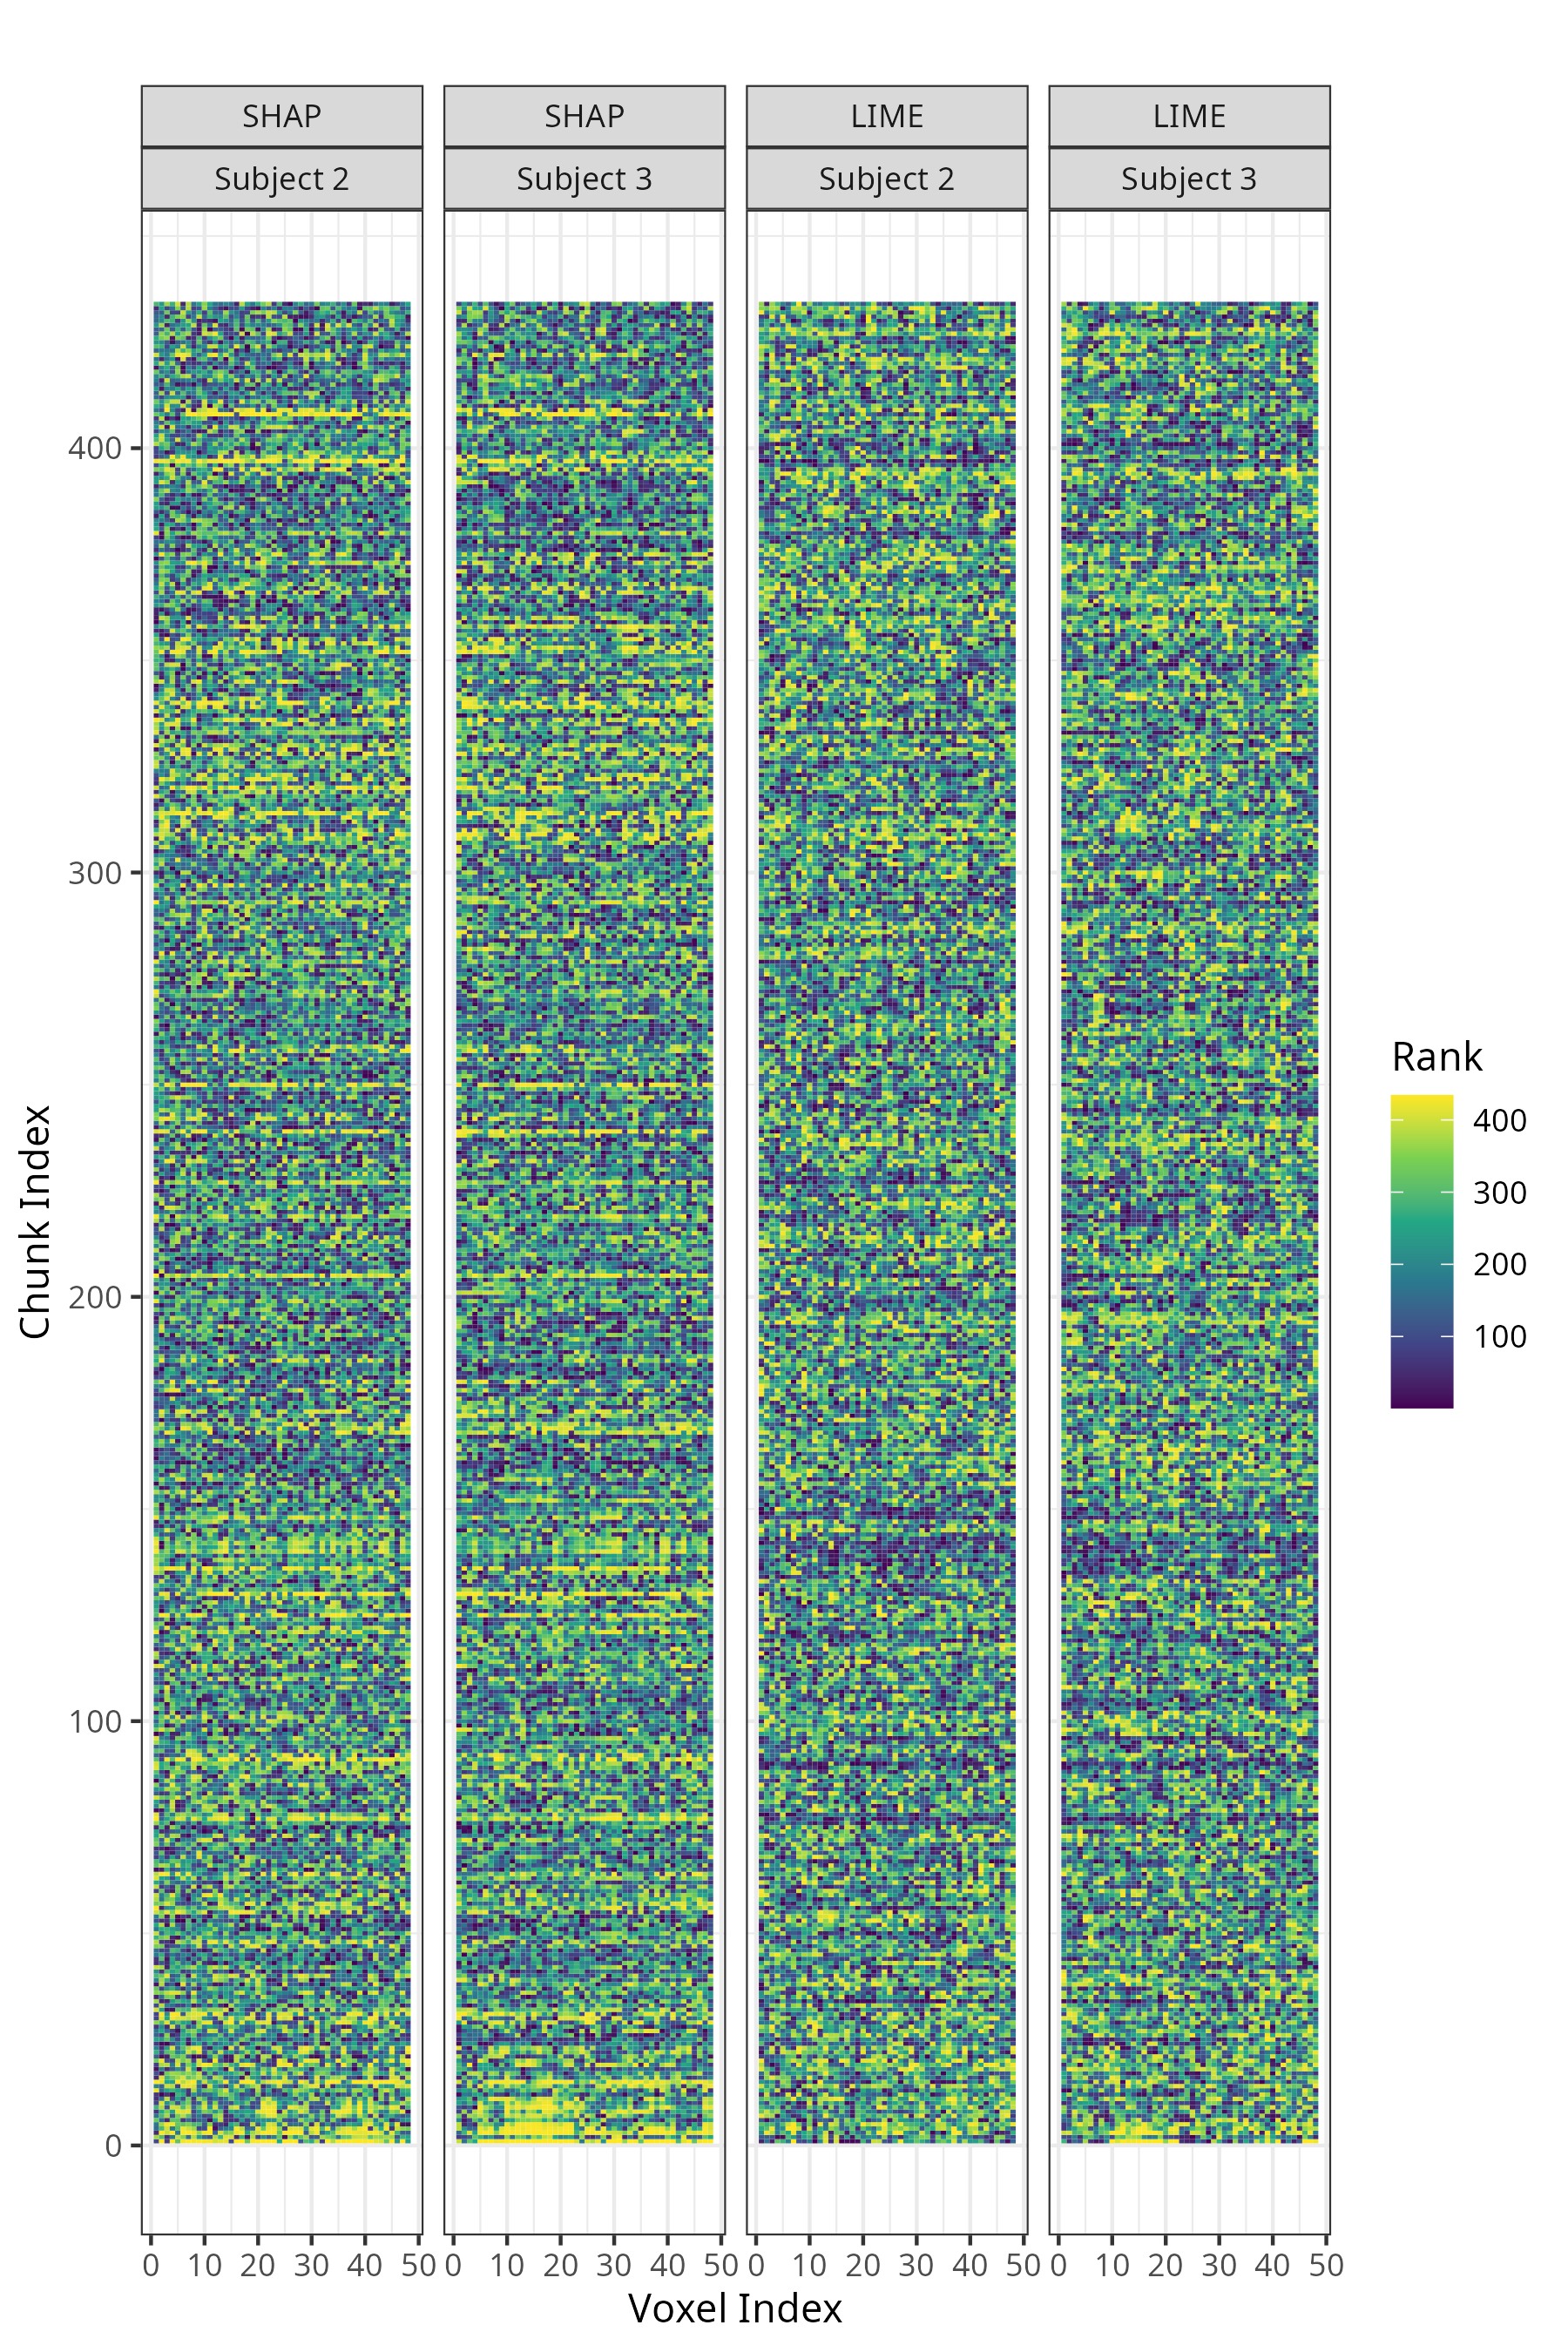
\includegraphics[width=\textwidth]{figs/heatmap_laws.png}
        \label{subfig:heatmap_laws}
    \end{subfigure}
    \hfill
    \begin{subfigure}[t]{0.35\textwidth}
        \centering
        \caption{Interquartile Range of Word Ranks}
        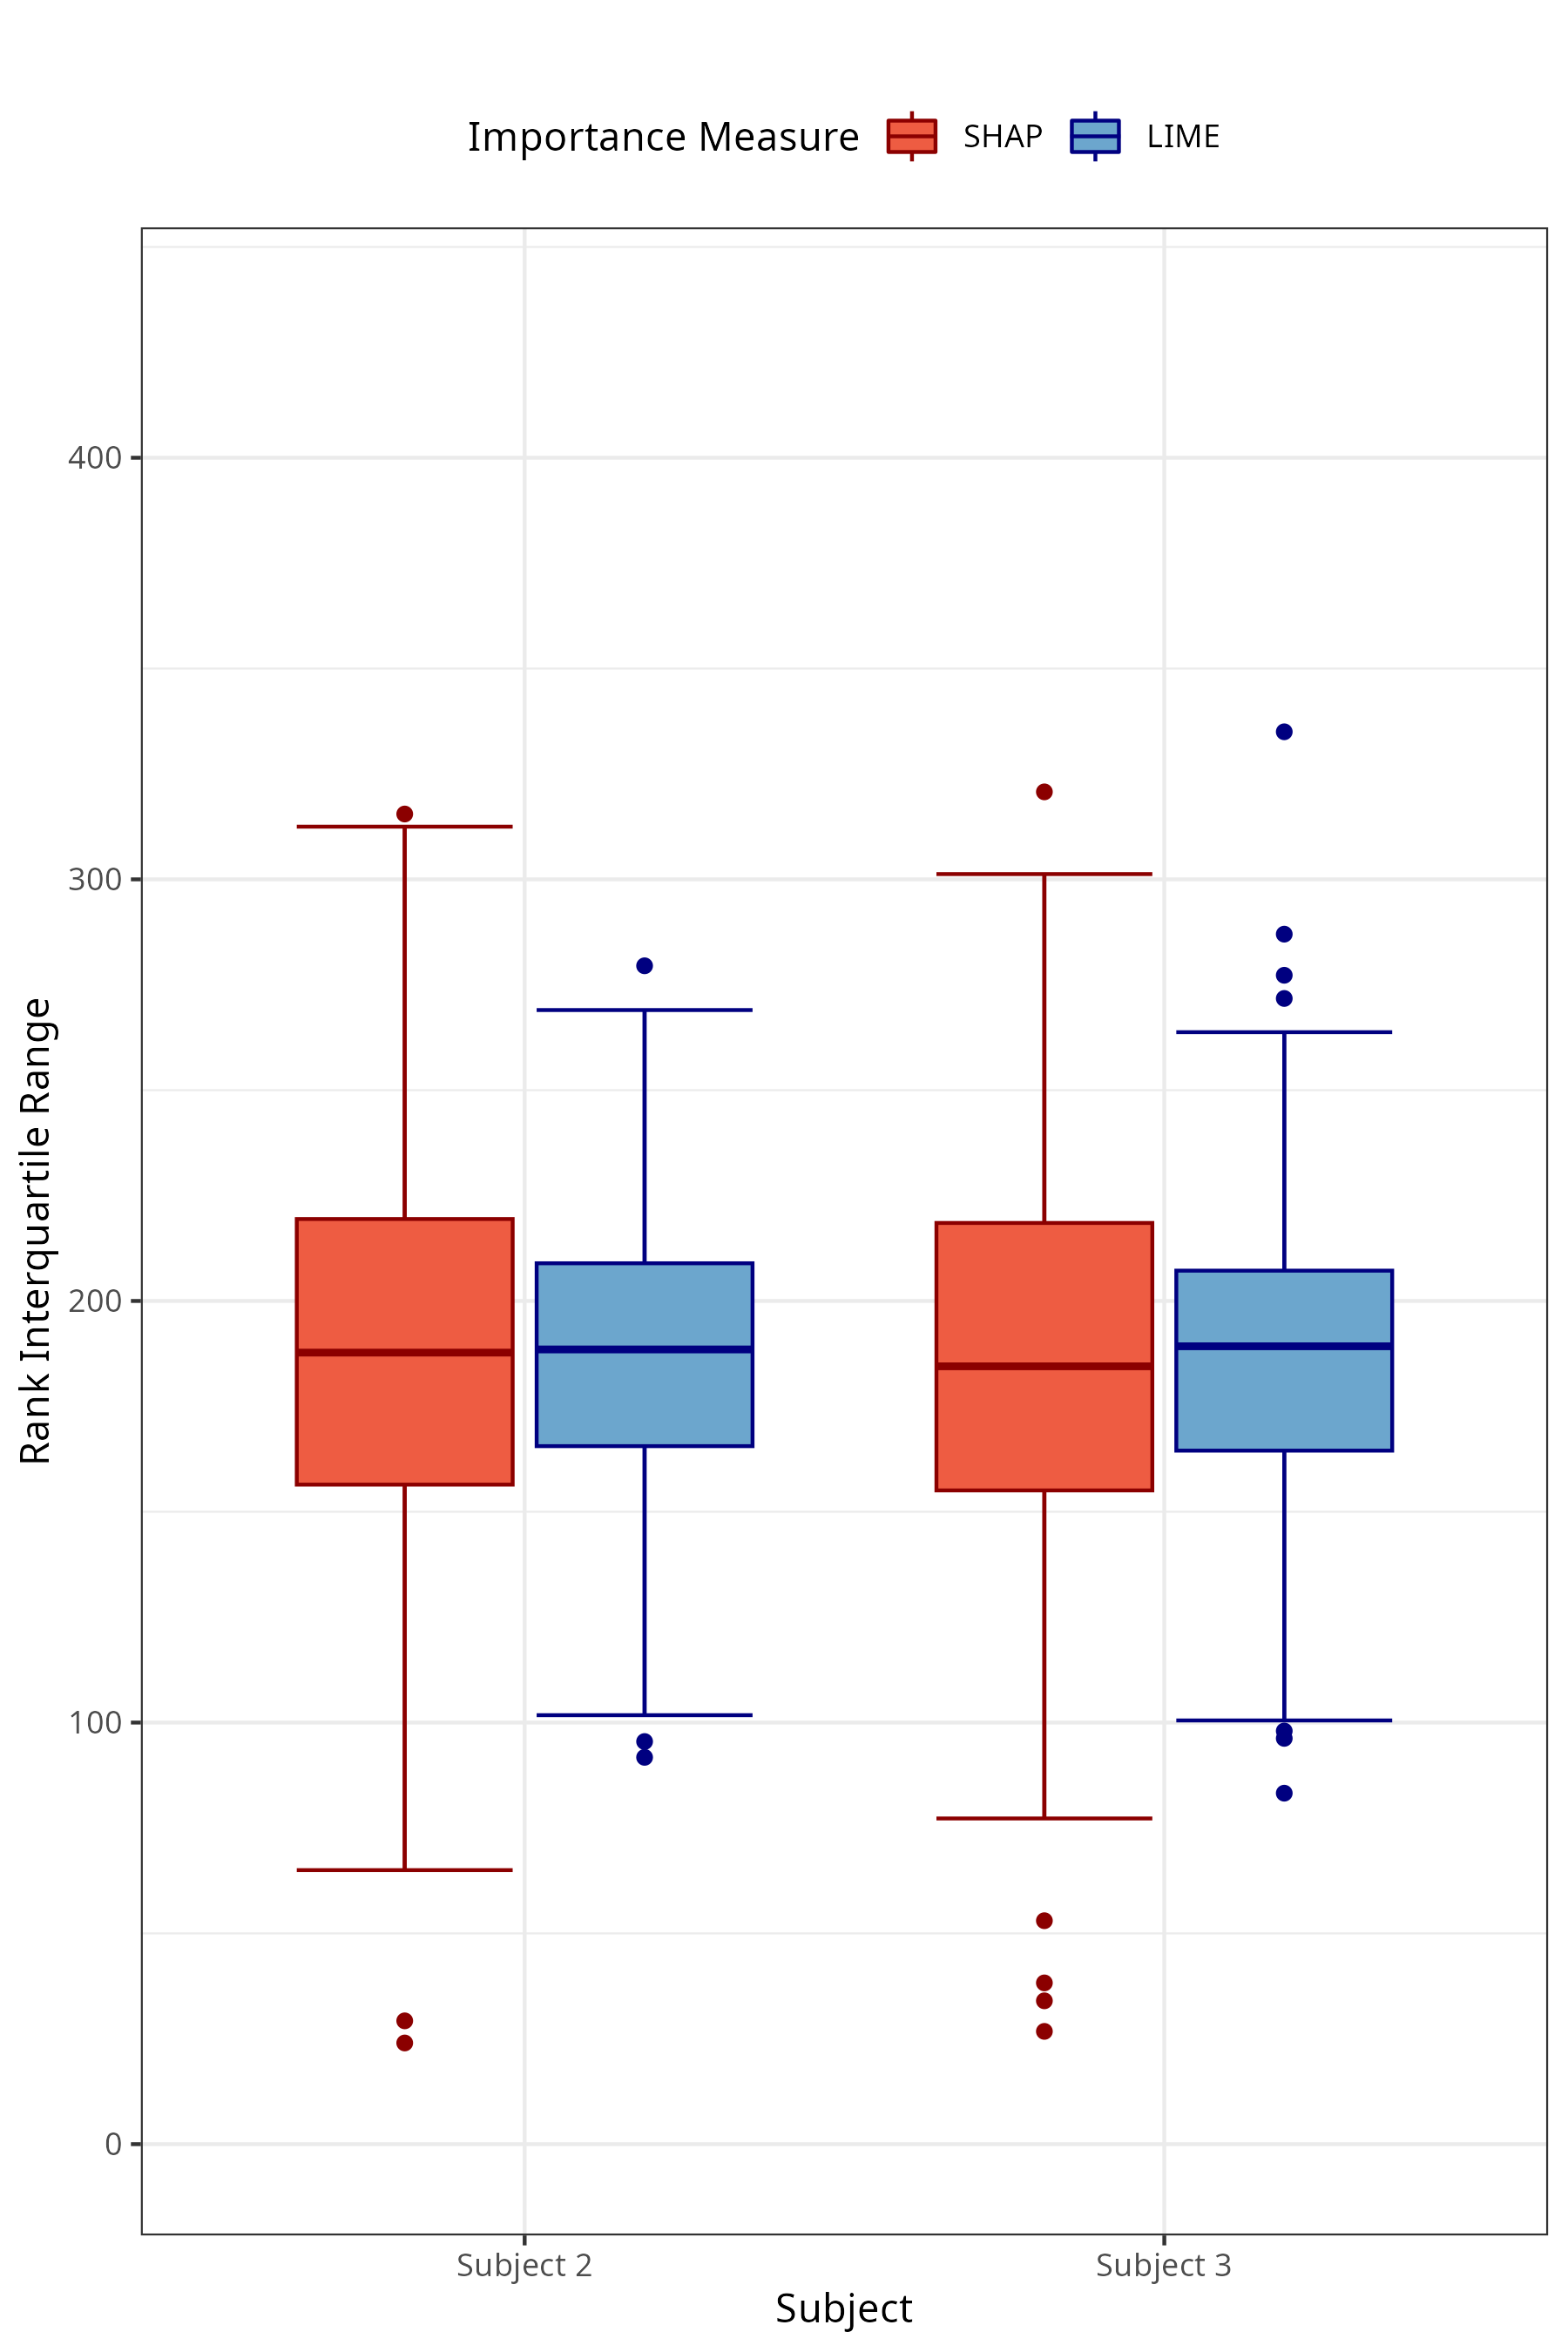
\includegraphics[width=\textwidth]{figs/boxplot_laws.png}
        \label{subfig:boxplot_laws}
    \end{subfigure}
    \caption{Word ranks assigned by individual voxels show a high degree of consistency within and across subjects. The heatmap (left) displays voxelwise rankings for 434 word chunks, revealing horizontal banding patterns that reflect agreement in word importance. The boxplot (right) summarizes the spread of these ranks within chunks. For the average word, the IQR spans only ${\sim}180$ ranks, suggesting relatively stable importance scores across voxels.}
    \label{fig:laws_voxelwise}
\end{figure}

\newpage

However, words identified by both methods include:
\begin{itemize}
    \item \textbf{Key thesis statements} (e.g., "i'm gonna tell you three stories", "now so instead what we need is")
    \item \textbf{Narrative transitions} (e.g., "and that's where the story of", "extremism on the other a fact we should have many many")
    \item \textbf{Opinion indicators} (e.g., "i think much more important much", "to fight for i as any good")
\end{itemize}

This pattern suggests that fMRI responses may be driven by both specific semantic content (captured by SHAP) and broader narrative structure (captured by LIME), reflecting the multi-level processing that occurs in the brain during language comprehension. For a more comprehensive list of words identified by each method, see Appendix \ref{sec:laws_text}.

Regarding differences across voxels, Figure \ref{fig:laws_voxelwise} reveals visible horizontal banding in the heatmaps for both SHAP and LIME, indicating that word rankings are relatively consistent across voxels within and between subjects. The accompanying boxplot shows that SHAP produces slightly lower median IQRs for word ranks across voxels, suggesting less variability and lower voxel sensitivity for the average word. Conversely, LIME exhibits a tighter distribution of IQR values, indicating that while its average variability may be higher, the spread among the least consistently ranked words is smaller.



\section{Conclusion}

This lab demonstrated the efficacy of leveraging pre-trained language models for predicting fMRI responses to narrative stimuli. Our experiments focused on utilizing BERT, first with static embeddings and then through parameter-efficient fine-tuning using LoRA.

The results indicate that embeddings from the pre-trained BERT model significantly outperform those from earlier labs (custom encoders or simpler static embeddings like Bag-of-Words) for Subject 2, and show competitive results for Subject 3. This highlights the benefit of the rich contextual representations learned by larger models. Furthermore, fine-tuning these BERT embeddings with LoRA provided an additional, albeit modest, improvement in predictive accuracy across both subjects, underscoring the value of task-specific adaptation even with limited trainable parameters. The choice of LoRA rank (\(r=8\)) and initializing regression heads from prior experiments proved beneficial.

Interpretability analysis using SHAP and LIME on the fine-tuned LoRA-BERT model identified words relevant to the narrative content that influenced predictions for well-modeled voxels. While SHAP and LIME offered somewhat divergent perspectives—SHAP often emphasizing thematic content and LIME highlighting structural or specific details—their combined insights suggest that the model attends to various meaningful linguistic features. Word importance showed reasonable consistency across subjects and voxels, indicating some shared neural processing patterns captured by the model.

In summary, this work confirms that pre-trained transformers, further refined with techniques like LoRA, provide a robust framework for modeling neural language processing. They offer improved predictive power and, through interpretability methods, can shed light on the linguistic features driving brain activity.

\newpage


\printbibliography

\appendix
\section{Academic honesty}
\subsection{Statement}
We affirm that the work in this report is entirely my own. We have not copied from any unauthorized sources, and all contributions from classmates, external sources, or tools are acknowledged. Academic research honesty is necessary because it ensures fairness, builds trust in scholarly work, and reflects personal integrity. Misrepresenting work undermines academic standards and disrespects the time and effort of peers and educators. Maintaining honesty in research fosters a learning environment where collaboration and progress can thrive authentically.

\subsection{LLM Usage}

We used ChatGPT to assist in clarifying concepts, creating visualizations, checking grammar, and improving the structure of our explanations. No content of the report or code was generated by the LLM without our review, editing, and refinement. We ensured that all content was written and understood by us, and the LLM was used as a tool to enhance our work rather than replace our understanding, we take full responsibility for all content in the report.

\newpage

\section{\texttt{buck} Full Text} \label{sec:buck_text}

Words discovered by SHAP in \textcolor{Maroon}{red}, LIME in \textcolor{RoyalBlue}{blue}, or both in \textbf{bold}. Threshold based on $75^{th}$ percentile word ranks.

\vspace{1em}
\noindent
\begin{minipage}{\textwidth}
\scriptsize % \small, \footnotesize, \scriptsize, etc.
\begin{spacing}{1.0} % line spacing
\textcolor{Maroon}{so} \textcolor{RoyalBlue}{as} \textcolor{RoyalBlue}{i} \textcolor{RoyalBlue}{sit} \textcolor{RoyalBlue}{down} \textcolor{Maroon}{to} \textcolor{Maroon}{eat} \textcolor{Maroon}{from} \textcolor{Maroon}{this} \textcolor{Maroon}{spread} \textcolor{Maroon}{that} \textcolor{Maroon}{has} \textcolor{Maroon}{been} \textcolor{Maroon}{given} in my honor i can't help but to f notice the two feelings that i'm having one i'm a little nervous two i'm very excited \textcolor{RoyalBlue}{because} \textcolor{RoyalBlue}{you} \textcolor{RoyalBlue}{see} in the morning i'll be paroling from state prison \textcolor{RoyalBlue}{after} \textcolor{RoyalBlue}{twenty} \textcolor{RoyalBlue}{six} \textcolor{RoyalBlue}{years} this spread is given \textcolor{Maroon}{to} \textcolor{Maroon}{me} \textcolor{Maroon}{not} \textcolor{Maroon}{as} \textcolor{Maroon}{like} \textcolor{Maroon}{to} \textcolor{Maroon}{say} \textcolor{Maroon}{hey} homie we appreciate you nah it was \textcolor{Maroon}{a} \textcolor{Maroon}{spread} \textcolor{Maroon}{to} \textcolor{Maroon}{say} \textcolor{Maroon}{we} \textcolor{Maroon}{don't} \textcolor{Maroon}{never} \textcolor{Maroon}{wanna} \textcolor{RoyalBlue}{see} \textcolor{RoyalBlue}{your} \textcolor{RoyalBlue}{ass} \textcolor{RoyalBlue}{in} \textcolor{RoyalBlue}{here} \textcolor{RoyalBlue}{again} and they broke \textcolor{Maroon}{out} \textcolor{Maroon}{the} \textcolor{Maroon}{finest} \textcolor{Maroon}{of} \textcolor{Maroon}{the} \textcolor{Maroon}{finest} \textcolor{Maroon}{top} \textcolor{Maroon}{ramen} \textcolor{RoyalBlue}{chili} \textcolor{RoyalBlue}{in} \textcolor{RoyalBlue}{a} \textcolor{RoyalBlue}{can} uh roast beef in \textcolor{RoyalBlue}{a} \textcolor{RoyalBlue}{can} \textcolor{RoyalBlue}{you} \textcolor{RoyalBlue}{know} \textcolor{RoyalBlue}{this} \textcolor{RoyalBlue}{this} \textcolor{RoyalBlue}{top} \textcolor{RoyalBlue}{line} \textcolor{RoyalBlue}{of} \textcolor{RoyalBlue}{stuff} \textcolor{RoyalBlue}{right} \textcolor{Maroon}{so} \textcolor{RoyalBlue}{after} \textcolor{RoyalBlue}{the} \textcolor{RoyalBlue}{spread} \textcolor{RoyalBlue}{has} \textcolor{RoyalBlue}{been} had \textcolor{Maroon}{it's} \textcolor{Maroon}{time} \textcolor{Maroon}{for} \textcolor{Maroon}{me} \textcolor{Maroon}{to} \textcolor{Maroon}{give} \textcolor{Maroon}{away} \textcolor{Maroon}{some} \textcolor{Maroon}{property} \textcolor{RoyalBlue}{such} \textcolor{RoyalBlue}{as} \textcolor{RoyalBlue}{my} \textcolor{RoyalBlue}{tv} \textcolor{RoyalBlue}{my} \textcolor{RoyalBlue}{radio} \textcolor{RoyalBlue}{and} \textcolor{RoyalBlue}{some} \textcolor{RoyalBlue}{self} \textcolor{RoyalBlue}{help} \textcolor{RoyalBlue}{books} \textcolor{Maroon}{that} \textcolor{Maroon}{helped} \textcolor{Maroon}{me} \textcolor{Maroon}{a} \textcolor{Maroon}{lot} \textcolor{Maroon}{so} \textcolor{Maroon}{they'll} \textcolor{Maroon}{be} \textcolor{Maroon}{better} \textcolor{Maroon}{utilized} left behind nine o'clock rolls around \textcolor{RoyalBlue}{it's} \textcolor{RoyalBlue}{lights} \textcolor{RoyalBlue}{out} \textcolor{RoyalBlue}{you} \textcolor{Maroon}{don't} \textcolor{Maroon}{have} \textcolor{Maroon}{to} \textcolor{Maroon}{go} \textcolor{Maroon}{to} \textcolor{Maroon}{sleep} \textcolor{Maroon}{but} \textcolor{Maroon}{you} \textcolor{Maroon}{do} \textcolor{Maroon}{gotta} \textcolor{Maroon}{get} \textcolor{Maroon}{off} \textcolor{Maroon}{the} \textcolor{Maroon}{day} \textcolor{Maroon}{room} \textcolor{Maroon}{floor} it's cool by me i'm leaving in the morning so i may have gotten like three hours worth of sleep that night i slept ready roll and that means \textcolor{Maroon}{i} \textcolor{Maroon}{slept} \textcolor{Maroon}{with} \textcolor{Maroon}{my} \textcolor{Maroon}{clothes} \textcolor{Maroon}{on} \textcolor{Maroon}{so} \textcolor{Maroon}{once} \textcolor{Maroon}{they} \textcolor{Maroon}{call} \textcolor{Maroon}{my} \textcolor{Maroon}{name} \textcolor{Maroon}{i'm} \textcolor{Maroon}{out} \textcolor{Maroon}{of} \textcolor{Maroon}{there} \textcolor{Maroon}{bye} see you later so five forty five rolls around the night man says cyprien d \textcolor{RoyalBlue}{thirty} \textcolor{RoyalBlue}{seven} \textcolor{RoyalBlue}{eighty} \textcolor{RoyalBlue}{seven} \textcolor{RoyalBlue}{five} \textcolor{RoyalBlue}{report} to r and r i walk down that \textcolor{RoyalBlue}{corridor} \textcolor{RoyalBlue}{for} \textcolor{RoyalBlue}{the} \textcolor{RoyalBlue}{last} \textcolor{RoyalBlue}{time} \textcolor{Maroon}{walk} \textcolor{Maroon}{the} \textcolor{Maroon}{one} \textcolor{Maroon}{gate} \textcolor{Maroon}{after} \textcolor{Maroon}{another} \textcolor{Maroon}{till} \textcolor{Maroon}{i} \textcolor{Maroon}{get} \textcolor{Maroon}{to} \textcolor{RoyalBlue}{r} \textcolor{RoyalBlue}{and} \textcolor{RoyalBlue}{r} \textcolor{RoyalBlue}{and} \textcolor{RoyalBlue}{that's} \textcolor{RoyalBlue}{receiving} and release and i'm on the release end at this point \textcolor{RoyalBlue}{i} \textcolor{RoyalBlue}{get} \textcolor{RoyalBlue}{to} \textcolor{RoyalBlue}{r} \textcolor{RoyalBlue}{and} \textcolor{RoyalBlue}{r} and there's about seven \textcolor{RoyalBlue}{to} \textcolor{RoyalBlue}{six} \textcolor{RoyalBlue}{other} \textcolor{RoyalBlue}{guys} \textcolor{RoyalBlue}{waiting} \textcolor{RoyalBlue}{for} \textcolor{RoyalBlue}{the} \textcolor{RoyalBlue}{same} thing they start fingerprinting me mugshots and everything i'm cool like time to go so \textcolor{RoyalBlue}{they} \textcolor{RoyalBlue}{load} \textcolor{RoyalBlue}{us} \textcolor{RoyalBlue}{on} \textcolor{RoyalBlue}{a} \textcolor{RoyalBlue}{van} and we drive through one gate after \textcolor{RoyalBlue}{another} \textcolor{RoyalBlue}{gate} \textcolor{RoyalBlue}{till} \textcolor{RoyalBlue}{we} \textcolor{RoyalBlue}{get} \textcolor{RoyalBlue}{to} \textcolor{RoyalBlue}{the} \textcolor{RoyalBlue}{final} \textcolor{RoyalBlue}{gate} \textcolor{RoyalBlue}{the} \textcolor{RoyalBlue}{cop} \textcolor{RoyalBlue}{says} alright everybody off the van you'll step to the \textcolor{Maroon}{man} \textcolor{Maroon}{at} \textcolor{Maroon}{the} \textcolor{Maroon}{base} \textcolor{Maroon}{of} \textcolor{Maroon}{the} \textcolor{Maroon}{tower} \textcolor{Maroon}{there} and you'll give him some personal information so we did and he gave each man an envelope \textcolor{RoyalBlue}{with} \textcolor{RoyalBlue}{two} \textcolor{RoyalBlue}{hundred} \textcolor{RoyalBlue}{dollars} \textcolor{RoyalBlue}{in} \textcolor{RoyalBlue}{it} better known as gate money we all got back onto the van and drove \textcolor{RoyalBlue}{through} \textcolor{RoyalBlue}{that} \textcolor{RoyalBlue}{last} \textcolor{RoyalBlue}{gate} \textcolor{RoyalBlue}{we} \textcolor{RoyalBlue}{made} \textcolor{RoyalBlue}{it} \textcolor{RoyalBlue}{around} \textcolor{RoyalBlue}{to} \textcolor{RoyalBlue}{the} \textcolor{RoyalBlue}{visitor's} \textcolor{RoyalBlue}{parking} \textcolor{RoyalBlue}{lot} \textcolor{RoyalBlue}{and} \textcolor{RoyalBlue}{he} \textcolor{RoyalBlue}{asked} \textcolor{RoyalBlue}{is} \textcolor{RoyalBlue}{there} \textcolor{RoyalBlue}{anyone} \textcolor{RoyalBlue}{with} \textcolor{RoyalBlue}{a} \textcolor{RoyalBlue}{ride} i do i was \textcolor{Maroon}{the} \textcolor{Maroon}{only} \textcolor{Maroon}{one} \textcolor{Maroon}{to} \textcolor{Maroon}{get} \textcolor{Maroon}{off} \textcolor{Maroon}{the} \textcolor{Maroon}{van} \textcolor{RoyalBlue}{these} \textcolor{RoyalBlue}{other} \textcolor{RoyalBlue}{guys} \textcolor{RoyalBlue}{that} \textcolor{RoyalBlue}{two} \textcolor{RoyalBlue}{hundred} \textcolor{RoyalBlue}{dollar} \textcolor{RoyalBlue}{gate} \textcolor{RoyalBlue}{money} \textcolor{Maroon}{they} \textcolor{Maroon}{had} \textcolor{Maroon}{to} \textcolor{Maroon}{spend} \textcolor{Maroon}{it} \textcolor{Maroon}{on} \textcolor{Maroon}{buying} \textcolor{Maroon}{their} bus tickets maybe back to southern california \textcolor{RoyalBlue}{or} \textcolor{RoyalBlue}{even} \textcolor{RoyalBlue}{further} \textcolor{RoyalBlue}{up} \textcolor{RoyalBlue}{north} \textcolor{RoyalBlue}{but} \textcolor{RoyalBlue}{i} \textcolor{RoyalBlue}{was} \textcolor{RoyalBlue}{the} \textcolor{RoyalBlue}{lucky} \textcolor{RoyalBlue}{one} \textcolor{RoyalBlue}{my} \textcolor{RoyalBlue}{wife} \textcolor{RoyalBlue}{was} \textcolor{RoyalBlue}{waiting} \textcolor{RoyalBlue}{there} \textcolor{RoyalBlue}{with} \textcolor{RoyalBlue}{her} \textcolor{RoyalBlue}{camera} \textbf{i} \textbf{could} \textbf{see} \textbf{her} \textbf{she} \textbf{was} \textbf{snapping} \textbf{pictures} \textcolor{RoyalBlue}{of} \textcolor{RoyalBlue}{me} \textcolor{RoyalBlue}{like} \textcolor{RoyalBlue}{a} \textcolor{RoyalBlue}{paparazzi} \textcolor{RoyalBlue}{i} \textcolor{RoyalBlue}{walk} \textcolor{RoyalBlue}{briskly} \textcolor{RoyalBlue}{towards} \textcolor{RoyalBlue}{her} \textbf{gave} \textbf{her} \textbf{a} \textbf{quick} \textbf{kiss} \textbf{whispered} \textbf{in} \textcolor{Maroon}{her} \textcolor{Maroon}{ear} \textcolor{Maroon}{let's} \textcolor{Maroon}{get} \textcolor{Maroon}{out} \textcolor{Maroon}{of} \textcolor{Maroon}{here} \textcolor{Maroon}{before} \textcolor{Maroon}{they} \textcolor{Maroon}{say} we made a mistake we got in the car drove \textcolor{RoyalBlue}{away} \textcolor{RoyalBlue}{i} \textcolor{RoyalBlue}{saw} \textcolor{RoyalBlue}{a} \textcolor{RoyalBlue}{seven} \textcolor{RoyalBlue}{eleven} \textcolor{Maroon}{i} \textcolor{Maroon}{was} \textcolor{Maroon}{like} \textcolor{Maroon}{hey} \textcolor{Maroon}{babe} \textcolor{Maroon}{pull} \textcolor{Maroon}{over} \textcolor{Maroon}{lemme} \textcolor{RoyalBlue}{i} \textcolor{RoyalBlue}{wanna} \textcolor{RoyalBlue}{go} \textcolor{RoyalBlue}{in} \textcolor{RoyalBlue}{and} \textcolor{RoyalBlue}{get} \textcolor{RoyalBlue}{something} \textcolor{RoyalBlue}{so} \textcolor{RoyalBlue}{i} \textcolor{RoyalBlue}{went} \textcolor{RoyalBlue}{in} \textcolor{RoyalBlue}{and} \textcolor{RoyalBlue}{i} grabbed a pack of big red gum i hadn't had chewing \textcolor{RoyalBlue}{gum} \textcolor{RoyalBlue}{in} \textcolor{RoyalBlue}{twenty} \textcolor{RoyalBlue}{six} \textcolor{RoyalBlue}{years} big red was my favorite we got back in the car drove \textcolor{RoyalBlue}{away} \textcolor{RoyalBlue}{we} \textcolor{RoyalBlue}{were} \textcolor{RoyalBlue}{on} \textcolor{RoyalBlue}{the} \textcolor{RoyalBlue}{road} \textcolor{Maroon}{for} \textcolor{Maroon}{about} \textcolor{Maroon}{thirty} \textcolor{Maroon}{to} \textcolor{Maroon}{forty} \textcolor{Maroon}{five} \textcolor{Maroon}{minutes} and i s \textcolor{RoyalBlue}{i} \textcolor{RoyalBlue}{spotted} \textcolor{RoyalBlue}{a} \textcolor{RoyalBlue}{target} i said hey babe that's target i saw that on the uh tv pull over lemme i wanna go in there so we did \textcolor{RoyalBlue}{the} \textcolor{RoyalBlue}{first} \textcolor{RoyalBlue}{thing} \textcolor{RoyalBlue}{that} \textcolor{RoyalBlue}{caught} \textcolor{RoyalBlue}{my} \textcolor{RoyalBlue}{eye} \textcolor{RoyalBlue}{was} \textcolor{RoyalBlue}{how} big the shopping basket was it was bigger than the space that i had to store my personal property while in \textcolor{Maroon}{prison} i grabbed the basket and went down the aisle grabbing various things such as underwear socks t-shirt toothbrush toothpaste you name it i grabbed it well there goes that two hundred dollar gate money \textcolor{RoyalBlue}{so} \textcolor{RoyalBlue}{back} \textcolor{RoyalBlue}{in} \textcolor{RoyalBlue}{the} \textcolor{RoyalBlue}{car} my wife says so what do you want for dinner whoa \textcolor{Maroon}{she's} stumped me with that one because for twenty six years \textcolor{Maroon}{no} \textcolor{Maroon}{one} \textcolor{Maroon}{had} \textcolor{Maroon}{ever} \textcolor{Maroon}{asked} \textcolor{Maroon}{me} \textcolor{Maroon}{what} \textcolor{Maroon}{do} \textcolor{Maroon}{i} \textcolor{Maroon}{want} for dinner my dinner came through a thirteen by thirteen hole in the wall \textcolor{Maroon}{you} \textcolor{Maroon}{stick} \textcolor{Maroon}{your} \textcolor{Maroon}{hand} \textcolor{Maroon}{in} \textcolor{Maroon}{there} \textcolor{Maroon}{and} \textcolor{Maroon}{pull} \textcolor{Maroon}{out} \textcolor{Maroon}{a} \textcolor{Maroon}{tray} \textcolor{Maroon}{and} \textcolor{Maroon}{what's} \textcolor{Maroon}{ever} \textcolor{Maroon}{on} \textcolor{Maroon}{there} \textcolor{Maroon}{that's} \textcolor{Maroon}{what} \textcolor{Maroon}{you} \textcolor{Maroon}{eat} so she \textcolor{Maroon}{says} \textcolor{Maroon}{i} \textcolor{Maroon}{know} \textcolor{Maroon}{what} \textcolor{Maroon}{to} \textcolor{Maroon}{fix} \textcolor{Maroon}{so} \textcolor{Maroon}{she} \textcolor{Maroon}{drove} we made it to the grocery store went into the grocery store this gigantic store \textcolor{Maroon}{berkeley} \textcolor{Maroon}{bowl} \textcolor{Maroon}{so} i made it to the produce section \textcolor{Maroon}{i'm} \textcolor{Maroon}{stuck} \textcolor{RoyalBlue}{there} \textcolor{RoyalBlue}{are} \textcolor{RoyalBlue}{so} \textcolor{RoyalBlue}{many} \textcolor{RoyalBlue}{oranges} to choose from and the reason and i'm stuck just looking at the oranges is \textcolor{Maroon}{because} \textcolor{Maroon}{for} \textcolor{Maroon}{the} \textcolor{Maroon}{past} \textcolor{Maroon}{ten} \textcolor{Maroon}{years} \textcolor{Maroon}{in} \textcolor{Maroon}{prison} \textcolor{RoyalBlue}{they} \textcolor{RoyalBlue}{had} \textcolor{RoyalBlue}{taken} \textcolor{RoyalBlue}{oranges} \textcolor{RoyalBlue}{away} \textcolor{RoyalBlue}{from} \textcolor{RoyalBlue}{us} \textcolor{RoyalBlue}{because} \textcolor{RoyalBlue}{they} \textcolor{RoyalBlue}{were} \textcolor{RoyalBlue}{used} \textcolor{RoyalBlue}{to} \textcolor{RoyalBlue}{make} wine \textcolor{Maroon}{so} there's like a bumpy orange \textcolor{RoyalBlue}{a} \textcolor{RoyalBlue}{smooth} \textcolor{RoyalBlue}{orange} \textcolor{RoyalBlue}{a} \textcolor{RoyalBlue}{navel} \textcolor{RoyalBlue}{orange} i even met my first blood orange and at the same time this wave hit me of alone and feeling like \textcolor{RoyalBlue}{i} \textcolor{RoyalBlue}{don't} \textcolor{RoyalBlue}{know} \textcolor{RoyalBlue}{a} \textcolor{RoyalBlue}{nervous} \textcolor{RoyalBlue}{feeling} \textcolor{RoyalBlue}{hit} \textcolor{RoyalBlue}{me} \textcolor{RoyalBlue}{like} i'm the only person in this store who's paroled from a prison today after twenty six years \textcolor{RoyalBlue}{i'm} \textcolor{RoyalBlue}{a} \textcolor{RoyalBlue}{little} \textcolor{RoyalBlue}{stuck} \textcolor{RoyalBlue}{a} \textcolor{RoyalBlue}{little} \textcolor{Maroon}{so} i'm looking around and i spot \textcolor{RoyalBlue}{this} \textcolor{RoyalBlue}{ink} \textcolor{RoyalBlue}{work} \textcolor{RoyalBlue}{it's} not the typical ink work that i see out here now like with colors no i \textcolor{Maroon}{know} \textcolor{Maroon}{this} \textcolor{Maroon}{ink} \textcolor{Maroon}{work} \textcolor{Maroon}{this} \textcolor{Maroon}{is} \textcolor{Maroon}{prison} \textcolor{Maroon}{ink} he has a prison \textcolor{RoyalBlue}{guard} \textcolor{RoyalBlue}{tower} \textcolor{RoyalBlue}{on} \textcolor{RoyalBlue}{him} \textcolor{RoyalBlue}{a} \textcolor{RoyalBlue}{meltic} clock with time i know that work i've seen that many times \textcolor{Maroon}{so} \textcolor{Maroon}{i} \textcolor{Maroon}{walk} \textcolor{Maroon}{over} \textcolor{Maroon}{to} \textcolor{Maroon}{him} \textcolor{Maroon}{and} \textcolor{Maroon}{i} \textcolor{Maroon}{whisper} \textcolor{RoyalBlue}{so} \textcolor{RoyalBlue}{what} \textcolor{RoyalBlue}{yard} \textcolor{RoyalBlue}{did} \textcolor{RoyalBlue}{you} \textcolor{RoyalBlue}{parole} from he said oh me i got i paroled from pelican bay like four months ago i'm \textcolor{RoyalBlue}{like} \textcolor{RoyalBlue}{and} \textcolor{RoyalBlue}{they} \textcolor{RoyalBlue}{know} \textcolor{RoyalBlue}{you} \textcolor{RoyalBlue}{got} \textcolor{RoyalBlue}{out} \textcolor{Maroon}{of} \textcolor{Maroon}{prison} \textcolor{Maroon}{they} \textcolor{Maroon}{know} \textcolor{Maroon}{you} \textcolor{Maroon}{on} \textcolor{Maroon}{parole} \textcolor{Maroon}{aw} \textcolor{Maroon}{yeah} \textcolor{Maroon}{they} \textcolor{Maroon}{not} \textcolor{Maroon}{tripping} \textcolor{Maroon}{here} \textcolor{Maroon}{this} \textcolor{Maroon}{is} \textcolor{Maroon}{berkeley} \textcolor{Maroon}{man} \textcolor{Maroon}{nah} \textcolor{Maroon}{nobody's} tripping \textcolor{Maroon}{well} i walked away from him with the understanding that if he \textcolor{RoyalBlue}{can} \textcolor{RoyalBlue}{get} \textcolor{RoyalBlue}{a} \textcolor{RoyalBlue}{job} \textcolor{RoyalBlue}{so} \textcolor{RoyalBlue}{can} \textcolor{RoyalBlue}{i} so i met my wife at the checkout once again there's another \textcolor{RoyalBlue}{stunned} \textcolor{RoyalBlue}{moment} \textcolor{RoyalBlue}{for} \textcolor{RoyalBlue}{me} there are twelve checkout lines and there's somebody on the other end bagging the groceries in prison there was one window maybe thirteen by thirteen again and there was like three \textcolor{Maroon}{hundred} \textcolor{Maroon}{guys} \textcolor{Maroon}{waiting} \textcolor{Maroon}{to} \textcolor{Maroon}{get} \textcolor{Maroon}{into} \textcolor{Maroon}{this} \textcolor{Maroon}{one} window with their lists i didn't have to worry about an alarm going off or anything no getting down we're gonna get our groceries \textcolor{Maroon}{and} \textcolor{Maroon}{leave} \textcolor{Maroon}{out} \textcolor{Maroon}{of} \textcolor{Maroon}{here} \textcolor{Maroon}{that} \textcolor{Maroon}{was} \textcolor{Maroon}{my} \textcolor{Maroon}{thought} cool so we made it through the made it \textcolor{Maroon}{through} \textcolor{Maroon}{the} \textcolor{Maroon}{checkout} \textcolor{Maroon}{went} \textcolor{Maroon}{back} \textcolor{Maroon}{to} \textcolor{Maroon}{the} \textcolor{Maroon}{car} \textcolor{Maroon}{got} \textcolor{Maroon}{in} \textcolor{Maroon}{the} \textcolor{Maroon}{car} \textcolor{Maroon}{and} \textcolor{Maroon}{we're} \textcolor{Maroon}{on} \textcolor{Maroon}{the} \textcolor{Maroon}{road} \textcolor{RoyalBlue}{and} \textcolor{RoyalBlue}{we} \textcolor{RoyalBlue}{come} \textcolor{RoyalBlue}{to} \textcolor{RoyalBlue}{a} \textcolor{RoyalBlue}{stoplight} \textcolor{Maroon}{and} this homeless guy had a sign that says anything \textcolor{RoyalBlue}{will} \textcolor{RoyalBlue}{help} \textcolor{RoyalBlue}{so} \textcolor{RoyalBlue}{my} \textcolor{RoyalBlue}{wife} \textcolor{Maroon}{reaches} \textcolor{Maroon}{into} \textcolor{Maroon}{the} \textcolor{Maroon}{cup} \textcolor{Maroon}{holder} \textcolor{Maroon}{and} \textcolor{RoyalBlue}{gets} \textcolor{RoyalBlue}{ready} \textcolor{RoyalBlue}{to} \textcolor{RoyalBlue}{hand} \textcolor{RoyalBlue}{him} \textcolor{RoyalBlue}{some} \textcolor{RoyalBlue}{change} \textcolor{Maroon}{and} \textcolor{Maroon}{all} \textcolor{Maroon}{of} \textcolor{Maroon}{a} \textcolor{Maroon}{sudden} \textcolor{Maroon}{he} \textcolor{Maroon}{gets} a phone call \textbf{and} \textbf{he} \textbf{tells} \textbf{my} \textbf{wife} \textbf{wait} \textcolor{RoyalBlue}{i} \textcolor{RoyalBlue}{gotta} \textcolor{RoyalBlue}{take} \textcolor{RoyalBlue}{this} \textcolor{RoyalBlue}{call} and my thoughts \textcolor{RoyalBlue}{was} \textcolor{RoyalBlue}{like} \textcolor{RoyalBlue}{ih} \textcolor{RoyalBlue}{if} \textcolor{RoyalBlue}{he} \textcolor{RoyalBlue}{got} \textcolor{RoyalBlue}{a} \textcolor{RoyalBlue}{cellphone} \textcolor{RoyalBlue}{i} \textcolor{RoyalBlue}{gotta} \textcolor{RoyalBlue}{get} \textcolor{RoyalBlue}{one} \textcolor{Maroon}{so} we drive away \textcolor{RoyalBlue}{and} \textcolor{RoyalBlue}{my} \textcolor{RoyalBlue}{wife} \textcolor{RoyalBlue}{uh} \textcolor{RoyalBlue}{she} \textcolor{RoyalBlue}{just} \textcolor{RoyalBlue}{drives} \textcolor{RoyalBlue}{real} \textcolor{RoyalBlue}{fast} \textcolor{RoyalBlue}{right} \textcolor{RoyalBlue}{and} \textcolor{RoyalBlue}{we} \textcolor{RoyalBlue}{make} \textcolor{Maroon}{it} \textcolor{Maroon}{to} \textcolor{Maroon}{the} \textcolor{Maroon}{neighborhood} \textcolor{Maroon}{just} \textcolor{Maroon}{as} \textcolor{Maroon}{fast} \textcolor{Maroon}{as} \textcolor{Maroon}{we} \textcolor{Maroon}{got} \textcolor{RoyalBlue}{to} \textcolor{RoyalBlue}{the} \textcolor{RoyalBlue}{store} \textcolor{RoyalBlue}{and} \textcolor{RoyalBlue}{she} \textcolor{Maroon}{pulls} \textcolor{Maroon}{into} \textcolor{Maroon}{the} \textcolor{Maroon}{neighborhood} \textcolor{Maroon}{and} \textcolor{Maroon}{she} \textcolor{Maroon}{points} \textcolor{Maroon}{out} \textcolor{Maroon}{the} various neighbors' house um this is \textcolor{Maroon}{where} \textcolor{Maroon}{fred} \textcolor{Maroon}{and} \textcolor{Maroon}{mike} \textcolor{Maroon}{live} \textcolor{Maroon}{the} \textcolor{Maroon}{brewers} \textcolor{Maroon}{live} here and i'm like okay \textcolor{Maroon}{and} \textcolor{Maroon}{we} \textcolor{Maroon}{get} \textcolor{Maroon}{to} \textcolor{Maroon}{our} \textcolor{Maroon}{house} \textcolor{Maroon}{and} \textcolor{Maroon}{she} \textcolor{Maroon}{said} \textcolor{Maroon}{this} \textcolor{Maroon}{is} \textcolor{Maroon}{us} \textcolor{Maroon}{and} \textcolor{Maroon}{we} \textcolor{Maroon}{live} \textcolor{Maroon}{at} \textcolor{Maroon}{the} \textcolor{Maroon}{edge} \textcolor{Maroon}{of} \textcolor{Maroon}{the} \textcolor{Maroon}{forest} i'm like cool cool \textcolor{RoyalBlue}{and} \textcolor{RoyalBlue}{so} \textcolor{RoyalBlue}{we} \textcolor{RoyalBlue}{went} \textcolor{RoyalBlue}{inside} and she gives me the grand tour and so she says well i'm gonna prepare this dinner i said cool so she made steak and lobster with small potatoes nothing out of a can folks nothing out of a packet either she made \textcolor{RoyalBlue}{this} \textcolor{RoyalBlue}{meal} \textcolor{RoyalBlue}{we} \textcolor{RoyalBlue}{sat} \textcolor{RoyalBlue}{down} \textcolor{RoyalBlue}{we} ate and i had \textcolor{RoyalBlue}{my} \textcolor{RoyalBlue}{first} \textcolor{RoyalBlue}{glass} \textcolor{RoyalBlue}{of} \textcolor{RoyalBlue}{wine} with my meal \textcolor{RoyalBlue}{not} \textcolor{RoyalBlue}{them} \textcolor{RoyalBlue}{i'm} \textcolor{RoyalBlue}{not} \textcolor{RoyalBlue}{saying} \textcolor{RoyalBlue}{i've} \textcolor{RoyalBlue}{never} \textcolor{Maroon}{had} \textcolor{Maroon}{wine} \textcolor{Maroon}{before} \textcolor{Maroon}{i've} \textcolor{Maroon}{never} \textcolor{Maroon}{had} \textcolor{Maroon}{wine} with a meal \textcolor{Maroon}{this} \textcolor{RoyalBlue}{is} \textcolor{RoyalBlue}{some} \textcolor{RoyalBlue}{grown} \textcolor{RoyalBlue}{folks'} \textcolor{RoyalBlue}{shit} \textcolor{RoyalBlue}{i} \textcolor{RoyalBlue}{thought} \textcolor{Maroon}{right} so after the meal was finished we're cleaning up \textcolor{RoyalBlue}{washing} \textcolor{RoyalBlue}{dishes} \textcolor{RoyalBlue}{my} \textcolor{RoyalBlue}{wife} \textcolor{RoyalBlue}{says} \textcolor{RoyalBlue}{you} \textcolor{RoyalBlue}{wanna} \textcolor{RoyalBlue}{get} \textcolor{RoyalBlue}{further} \textcolor{RoyalBlue}{acclimated} i'm like yeah she said take out the garbage no problem i reach down tie that garbage bag \textcolor{Maroon}{up} \textcolor{Maroon}{throw} \textcolor{Maroon}{it} \textcolor{Maroon}{over} \textcolor{Maroon}{my} \textcolor{Maroon}{shoulder} \textcolor{Maroon}{and} \textcolor{Maroon}{out} \textcolor{RoyalBlue}{to} \textcolor{RoyalBlue}{the} \textcolor{RoyalBlue}{front} \textcolor{RoyalBlue}{door} \textcolor{RoyalBlue}{i} \textcolor{RoyalBlue}{go} when i open up the door \textcolor{RoyalBlue}{no} \textcolor{RoyalBlue}{more} \textcolor{RoyalBlue}{than} \textcolor{RoyalBlue}{eight} \textcolor{RoyalBlue}{feet} \textcolor{RoyalBlue}{away} from me was a ten point buck \textcolor{Maroon}{just} standing there looking at me look at it standing staring at me \textcolor{RoyalBlue}{now} \textcolor{RoyalBlue}{had} \textcolor{RoyalBlue}{we} \textcolor{RoyalBlue}{been} \textcolor{RoyalBlue}{on} \textcolor{RoyalBlue}{a} \textcolor{RoyalBlue}{prison} \textbf{yard} \textbf{me} \textbf{and} \textbf{this} \textbf{buck} \textbf{woulda} \textbf{had} \textbf{issues} \textcolor{Maroon}{now} \textcolor{Maroon}{i} \textcolor{Maroon}{speak} \textcolor{Maroon}{a} \textcolor{Maroon}{lot} \textcolor{Maroon}{of} \textcolor{Maroon}{different} \textcolor{Maroon}{gangster} \textcolor{Maroon}{languages} \textcolor{RoyalBlue}{i'm} \textcolor{RoyalBlue}{fluent} \textcolor{RoyalBlue}{in} \textcolor{RoyalBlue}{crip} \textcolor{RoyalBlue}{i} \textcolor{Maroon}{understand} \textcolor{Maroon}{blood} \textcolor{Maroon}{i} \textcolor{Maroon}{even} \textcolor{Maroon}{speak} \textcolor{Maroon}{a} \textcolor{Maroon}{little} \textcolor{RoyalBlue}{sh} \textcolor{RoyalBlue}{olo} \textcolor{RoyalBlue}{vato} \textcolor{RoyalBlue}{loco} but i don't speak deer so \textcolor{RoyalBlue}{i} \textcolor{RoyalBlue}{shut} \textcolor{RoyalBlue}{the} \textcolor{RoyalBlue}{door} \textcolor{RoyalBlue}{i} \textbf{call} \textbf{out} \textbf{to} \textbf{my} \textbf{wife} \textbf{i} \textbf{said} \textbf{hey} \textbf{babe} there's somebody here to see you \textcolor{RoyalBlue}{she} \textcolor{RoyalBlue}{came} \textcolor{RoyalBlue}{to} \textcolor{RoyalBlue}{the} \textcolor{RoyalBlue}{door} \textcolor{RoyalBlue}{opened} \textcolor{RoyalBlue}{it} and saw there was the buck \textcolor{RoyalBlue}{she} \textcolor{RoyalBlue}{grabbed} \textcolor{RoyalBlue}{the} \textcolor{RoyalBlue}{trashbag} \textcolor{RoyalBlue}{and} \textcolor{RoyalBlue}{walked} \textcolor{RoyalBlue}{right} past it i said damn she speaks deer she came back \textcolor{Maroon}{and} \textcolor{Maroon}{we} \textcolor{Maroon}{both} \textcolor{Maroon}{look} \textcolor{Maroon}{out} \textcolor{Maroon}{the} \textcolor{Maroon}{door} \textcolor{Maroon}{together} \textcolor{RoyalBlue}{at} \textcolor{RoyalBlue}{this} \textcolor{RoyalBlue}{buck} \textcolor{RoyalBlue}{who's} \textcolor{RoyalBlue}{still} \textcolor{RoyalBlue}{standing} \textcolor{RoyalBlue}{there} \textcolor{RoyalBlue}{just} \textcolor{RoyalBlue}{looking} \textcolor{RoyalBlue}{just} \textcolor{RoyalBlue}{majestic} as could be and my wife says you don't need to trip him \textcolor{Maroon}{he's} \textcolor{Maroon}{just} \textcolor{Maroon}{one} \textcolor{Maroon}{neighbor} \textcolor{Maroon}{coming} \textcolor{Maroon}{to} \textcolor{Maroon}{welcome} \textcolor{Maroon}{you} \textcolor{Maroon}{to} \textcolor{Maroon}{the} \textcolor{Maroon}{neighborhood} cool i thought like \textcolor{RoyalBlue}{well} \textcolor{RoyalBlue}{the} \textcolor{RoyalBlue}{fellas} \textcolor{RoyalBlue}{aren't} \textcolor{RoyalBlue}{gonna} believe this shit when i tell them this
\end{spacing}
\end{minipage}
\vspace{1em}

\newpage

\section{\texttt{lawsthatchokecreativity} Full Text} \label{sec:laws_text}

Words discovered by SHAP in \textcolor{Maroon}{red}, LIME in \textcolor{RoyalBlue}{blue}, or both in \textbf{bold}. Threshold based on $75^{th}$ percentile word ranks.

\vspace{1em}
\noindent
\begin{minipage}{\textwidth}
\ssmall % \small, \footnotesize, \scriptsize, etc.
\begin{spacing}{1.0} % line spacing
\textbf{i'm} \textbf{gonna} \textbf{tell} \textbf{you} \textbf{three} \textbf{stories} \textbf{on} \textbf{the} \textbf{way} \textbf{to} \textbf{one} argument that's \textbf{going} \textbf{to} \textbf{tell} \textbf{you} \textbf{a} \textbf{little} \textbf{bit} \textbf{about} \textbf{how} \textbf{we} \textbf{open} \textbf{user} \textbf{generated} \textbf{content} \textbf{up} \textbf{for} \textbf{business} \textbf{so} \textbf{here's} \textbf{the} first story \textcolor{Maroon}{nineteen} \textcolor{Maroon}{oh} \textcolor{Maroon}{six} \textcolor{Maroon}{this} \textcolor{Maroon}{man} \textcolor{Maroon}{john} \textcolor{Maroon}{philip} \textcolor{Maroon}{sousa} \textcolor{Maroon}{traveled} \textcolor{Maroon}{to} \textcolor{Maroon}{this} \textcolor{Maroon}{place} \textcolor{Maroon}{the} \textcolor{Maroon}{united} \textcolor{Maroon}{states} \textcolor{Maroon}{capitol} \textcolor{Maroon}{to} \textcolor{Maroon}{talk} \textcolor{Maroon}{about} \textcolor{Maroon}{this} \textbf{technology} \textbf{what} \textbf{he} \textbf{called} \textbf{the} \textbf{quote} talking machines \textcolor{Maroon}{sousa} \textcolor{Maroon}{was} \textcolor{Maroon}{not} \textbf{a} \textbf{fan} \textbf{of} \textbf{the} \textbf{talking} \textcolor{Maroon}{machines} \textcolor{Maroon}{this} \textcolor{Maroon}{is} \textcolor{Maroon}{what} \textcolor{Maroon}{he} \textcolor{Maroon}{had} \textcolor{Maroon}{to} \textcolor{Maroon}{say} \textcolor{Maroon}{these} talking machines are going to ruin artistic development of music \textcolor{RoyalBlue}{in} \textcolor{RoyalBlue}{this} \textcolor{RoyalBlue}{country} \textcolor{RoyalBlue}{when} \textbf{i} \textbf{was} \textbf{a} \textbf{boy} \textbf{in} \textbf{front} \textbf{of} \textbf{every} \textbf{house} \textbf{in} \textbf{the} \textbf{summer} \textbf{evenings} \textbf{you} would find young people together \textcolor{Maroon}{singing} \textcolor{Maroon}{the} \textcolor{Maroon}{songs} \textcolor{Maroon}{of} \textcolor{Maroon}{the} \textcolor{Maroon}{day} \textbf{or} \textbf{the} \textbf{old} \textbf{songs} today you hear these infernal machines going night \textcolor{RoyalBlue}{and} \textcolor{RoyalBlue}{day} \textcolor{RoyalBlue}{we} \textcolor{RoyalBlue}{will} \textcolor{RoyalBlue}{not} \textcolor{RoyalBlue}{have} \textcolor{RoyalBlue}{a} \textcolor{RoyalBlue}{vocal} \textcolor{RoyalBlue}{cord} \textcolor{RoyalBlue}{left} sousa said the vocal cords \textcolor{Maroon}{will} \textcolor{Maroon}{be} \textcolor{Maroon}{eliminated} \textcolor{Maroon}{by} \textcolor{Maroon}{a} \textcolor{Maroon}{process} \textcolor{Maroon}{of} \textcolor{Maroon}{evolution} \textbf{as} \textbf{was} \textbf{the} \textbf{tail} \textbf{of} \textcolor{Maroon}{man} \textcolor{Maroon}{when} \textcolor{Maroon}{he} \textcolor{Maroon}{came} \textcolor{Maroon}{from} \textcolor{Maroon}{the} \textcolor{Maroon}{ape} \textcolor{RoyalBlue}{this} \textcolor{RoyalBlue}{is} \textcolor{RoyalBlue}{a} \textcolor{RoyalBlue}{picture} \textcolor{RoyalBlue}{of} culture we could describe it using modern computer terminology as a kind of read write culture \textcolor{RoyalBlue}{it's} \textcolor{RoyalBlue}{a} \textcolor{RoyalBlue}{culture} \textcolor{RoyalBlue}{where} \textcolor{RoyalBlue}{people} \textcolor{RoyalBlue}{participate} \textcolor{RoyalBlue}{in} \textcolor{RoyalBlue}{the} \textcolor{RoyalBlue}{creation} \textcolor{RoyalBlue}{and} \textcolor{RoyalBlue}{the} \textcolor{RoyalBlue}{re} creation of their culture in that sense it's read write sousa's fear \textcolor{RoyalBlue}{was} \textcolor{RoyalBlue}{that} \textcolor{RoyalBlue}{we} \textcolor{RoyalBlue}{would} \textcolor{RoyalBlue}{lose} \textcolor{RoyalBlue}{that} capacity because of \textcolor{RoyalBlue}{these} \textcolor{RoyalBlue}{quote} \textcolor{RoyalBlue}{infernal} \textcolor{RoyalBlue}{machines} they would take it away and in its place we'd have the opposite \textcolor{Maroon}{of} \textcolor{Maroon}{read} \textcolor{Maroon}{write} \textcolor{Maroon}{culture} \textcolor{Maroon}{what} \textcolor{Maroon}{we} \textcolor{Maroon}{could} call read only culture culture where creativity was consumed but the consumer is not a creator \textcolor{RoyalBlue}{a} \textcolor{RoyalBlue}{culture} \textcolor{RoyalBlue}{which} \textcolor{RoyalBlue}{is} \textcolor{RoyalBlue}{top} \textcolor{RoyalBlue}{down} \textcolor{RoyalBlue}{owned} \textcolor{RoyalBlue}{where} \textcolor{RoyalBlue}{the} \textcolor{RoyalBlue}{vocal} \textcolor{Maroon}{cords} \textcolor{Maroon}{of} \textcolor{Maroon}{the} \textcolor{Maroon}{millions} \textcolor{Maroon}{have} \textcolor{Maroon}{been} \textcolor{Maroon}{lost} \textcolor{Maroon}{now} \textcolor{Maroon}{as} \textcolor{Maroon}{you} \textcolor{Maroon}{look} \textcolor{Maroon}{back} at the twentieth century \textcolor{Maroon}{at} \textcolor{Maroon}{least} \textcolor{Maroon}{in} \textcolor{Maroon}{what} \textcolor{Maroon}{we} \textcolor{Maroon}{think} \textcolor{RoyalBlue}{of} \textcolor{RoyalBlue}{as} \textcolor{RoyalBlue}{the} \textcolor{RoyalBlue}{quote} \textcolor{RoyalBlue}{developed} \textcolor{RoyalBlue}{world} hard not to conclude that sousa was right \textcolor{Maroon}{never} \textcolor{Maroon}{before} \textcolor{Maroon}{in} \textcolor{Maroon}{the} \textcolor{Maroon}{history} \textcolor{Maroon}{of} \textcolor{Maroon}{human} \textcolor{Maroon}{culture} \textcolor{Maroon}{had} \textcolor{Maroon}{it} \textcolor{RoyalBlue}{been} \textcolor{RoyalBlue}{as} \textcolor{RoyalBlue}{professionalized} \textcolor{RoyalBlue}{never} \textcolor{RoyalBlue}{before} as concentrated never before has creativity of the millions been as effectively displaced and displaced because of these quote infernal machines the twentieth century \textcolor{RoyalBlue}{was} \textcolor{RoyalBlue}{that} \textcolor{RoyalBlue}{century} \textcolor{RoyalBlue}{where} \textcolor{RoyalBlue}{at} \textcolor{RoyalBlue}{least} \textcolor{RoyalBlue}{for} \textcolor{RoyalBlue}{those} \textcolor{RoyalBlue}{places} \textcolor{RoyalBlue}{we} \textcolor{RoyalBlue}{know} \textcolor{RoyalBlue}{the} \textcolor{RoyalBlue}{best} culture moved from \textcolor{RoyalBlue}{this} \textcolor{RoyalBlue}{read} \textcolor{RoyalBlue}{write} \textcolor{RoyalBlue}{to} read only existence \textcolor{Maroon}{so} \textcolor{Maroon}{second} \textcolor{RoyalBlue}{{cg}} \textcolor{RoyalBlue}{land} \textcolor{RoyalBlue}{is} \textcolor{RoyalBlue}{a} \textcolor{RoyalBlue}{kind} \textcolor{RoyalBlue}{of} \textcolor{RoyalBlue}{property} is property it's protected by law \textcolor{Maroon}{as} \textcolor{Maroon}{lord} \textcolor{Maroon}{blackstone} \textcolor{RoyalBlue}{described} \textcolor{RoyalBlue}{it} \textcolor{RoyalBlue}{land} \textcolor{RoyalBlue}{is} \textcolor{RoyalBlue}{protected} by trespass law \textbf{for} \textbf{most} \textbf{of} \textbf{the} \textbf{history} \textbf{of} \textbf{trespass} law by presuming it protects the land all the way down below and to an indefinite \textcolor{Maroon}{extent} \textcolor{Maroon}{upwards} \textcolor{Maroon}{now} \textcolor{Maroon}{that} \textcolor{Maroon}{was} \textcolor{Maroon}{a} \textcolor{Maroon}{pretty} \textcolor{Maroon}{good} \textcolor{Maroon}{system} \textcolor{Maroon}{for} \textcolor{Maroon}{most} \textcolor{Maroon}{of} \textcolor{Maroon}{the} \textcolor{Maroon}{history} \textcolor{Maroon}{of} \textcolor{Maroon}{the} \textcolor{Maroon}{regulation} \textcolor{Maroon}{of} \textcolor{Maroon}{land} \textcolor{Maroon}{until} \textcolor{Maroon}{this} technology came along and people began to wonder were these \textcolor{Maroon}{instruments} \textcolor{Maroon}{trespassers} \textcolor{RoyalBlue}{as} \textcolor{RoyalBlue}{they} \textcolor{RoyalBlue}{flew} \textcolor{RoyalBlue}{over} \textcolor{RoyalBlue}{land} \textcolor{RoyalBlue}{without} \textcolor{RoyalBlue}{clearing} \textcolor{RoyalBlue}{the} \textcolor{RoyalBlue}{rights} \textcolor{RoyalBlue}{of} \textcolor{RoyalBlue}{the} \textcolor{RoyalBlue}{farms} below as they traveled \textcolor{RoyalBlue}{across} \textcolor{RoyalBlue}{the} \textcolor{RoyalBlue}{country} \textcolor{RoyalBlue}{well} \textcolor{RoyalBlue}{in} \textcolor{RoyalBlue}{nineteen} \textcolor{RoyalBlue}{forty} \textcolor{RoyalBlue}{five} \textcolor{RoyalBlue}{supreme} \textcolor{RoyalBlue}{court} \textcolor{RoyalBlue}{got} \textcolor{RoyalBlue}{a} \textcolor{RoyalBlue}{chance} \textcolor{RoyalBlue}{to} \textcolor{RoyalBlue}{address} \textcolor{RoyalBlue}{that} \textcolor{RoyalBlue}{question} two farmers thomas lee and tinie causby who raised chickens had a significant complaint because of these technologies \textcolor{RoyalBlue}{the} \textcolor{RoyalBlue}{complaint} \textcolor{RoyalBlue}{was} \textcolor{RoyalBlue}{that} \textcolor{RoyalBlue}{their} \textcolor{RoyalBlue}{chickens} followed the pattern \textcolor{Maroon}{of} \textcolor{Maroon}{the} \textcolor{Maroon}{airplanes} \textcolor{Maroon}{and} \textcolor{Maroon}{flew} \textcolor{Maroon}{themselves} \textcolor{Maroon}{into} the walls of the barn when the airplanes flew \textcolor{Maroon}{over} \textcolor{Maroon}{the} \textcolor{Maroon}{land} \textcolor{Maroon}{and} \textcolor{Maroon}{so} \textcolor{Maroon}{they} \textcolor{Maroon}{appealed} \textcolor{Maroon}{to} lord blackstone to say these airplanes were trespassing since time immemorial \textcolor{RoyalBlue}{the} \textcolor{RoyalBlue}{law} \textcolor{RoyalBlue}{had} \textcolor{RoyalBlue}{said} \textcolor{RoyalBlue}{you} \textcolor{RoyalBlue}{can't} fly over the land without permission of the landowner so this flight must \textcolor{Maroon}{stop} \textcolor{Maroon}{well} \textcolor{Maroon}{the} \textcolor{Maroon}{supreme} \textcolor{Maroon}{court} \textcolor{Maroon}{considered} \textcolor{RoyalBlue}{this} \textcolor{RoyalBlue}{hundred} \textcolor{RoyalBlue}{years} \textcolor{RoyalBlue}{tradition} and said \textbf{in} \textbf{an} \textbf{opinion} \textbf{written} \textbf{by} \textbf{justice} \textbf{douglas} that the causbys must lose the supreme court said the doctrine protecting land all the way to \textcolor{Maroon}{the} \textcolor{Maroon}{sky} \textcolor{Maroon}{has} \textcolor{Maroon}{no} \textcolor{Maroon}{place} \textcolor{Maroon}{in} \textcolor{Maroon}{the} \textcolor{Maroon}{modern} world otherwise every transcontinental flight would be \textcolor{RoyalBlue}{subject} \textcolor{RoyalBlue}{would} \textcolor{RoyalBlue}{subject} \textcolor{RoyalBlue}{the} \textcolor{RoyalBlue}{operator} to countless trespass suits \textcolor{Maroon}{common} \textcolor{Maroon}{sense} \textcolor{Maroon}{a} \textcolor{Maroon}{rare} \textcolor{Maroon}{idea} \textcolor{Maroon}{in} \textcolor{Maroon}{the} \textcolor{Maroon}{law} \textcolor{Maroon}{but} \textcolor{Maroon}{here} \textcolor{Maroon}{it} \textcolor{Maroon}{was} common sense revolts at the idea common sense \textcolor{Maroon}{{cg}} \textcolor{Maroon}{finally} \textcolor{Maroon}{{cg}} \textcolor{Maroon}{before} \textcolor{Maroon}{the} \textcolor{Maroon}{internet} the last great terror \textcolor{RoyalBlue}{to} \textcolor{RoyalBlue}{rain} \textcolor{RoyalBlue}{down} \textcolor{RoyalBlue}{on} the content industry \textcolor{RoyalBlue}{was} \textcolor{RoyalBlue}{a} \textcolor{RoyalBlue}{terror} \textcolor{RoyalBlue}{created} \textcolor{RoyalBlue}{by} \textcolor{RoyalBlue}{this} \textcolor{RoyalBlue}{technology} \textcolor{Maroon}{broadcasting} a new way to spread content and therefore a new \textcolor{Maroon}{battle} \textcolor{Maroon}{over} \textcolor{Maroon}{the} \textcolor{Maroon}{control} of the businesses that would spread content now at that time \textcolor{RoyalBlue}{the} \textcolor{RoyalBlue}{entity} \textcolor{RoyalBlue}{the} \textcolor{RoyalBlue}{legal} \textcolor{RoyalBlue}{cartel} that controlled the performance \textcolor{RoyalBlue}{rights} \textcolor{RoyalBlue}{for} \textcolor{RoyalBlue}{most} \textcolor{RoyalBlue}{of} \textcolor{RoyalBlue}{the} \textcolor{RoyalBlue}{music} \textcolor{RoyalBlue}{that} \textcolor{RoyalBlue}{would} \textcolor{RoyalBlue}{be} \textcolor{RoyalBlue}{broadcast} using these technologies was ascap they had an excusi \textcolor{RoyalBlue}{exclusive} \textcolor{RoyalBlue}{license} \textcolor{RoyalBlue}{on} \textcolor{RoyalBlue}{the} \textcolor{RoyalBlue}{most} popular content and they \textcolor{RoyalBlue}{exercised} \textcolor{RoyalBlue}{it} \textcolor{RoyalBlue}{in} \textcolor{RoyalBlue}{a} \textcolor{RoyalBlue}{way} that tried to demonstrate to the broadcasters who really was in charge so between nineteen \textbf{thirty} \textbf{one} \textbf{and} \textbf{nineteen} \textbf{thirty} \textbf{nine} \textbf{they} \textcolor{Maroon}{raised} \textcolor{Maroon}{rates} \textcolor{Maroon}{by} \textcolor{Maroon}{some} \textcolor{Maroon}{four} \textcolor{Maroon}{hundred} \textcolor{Maroon}{and} \textcolor{Maroon}{forty} \textcolor{Maroon}{eight} \textcolor{Maroon}{percent} \textcolor{RoyalBlue}{until} \textcolor{RoyalBlue}{the} \textcolor{RoyalBlue}{broadcasters} \textcolor{RoyalBlue}{finally} \textcolor{RoyalBlue}{got} \textcolor{RoyalBlue}{together} and said okay enough of this \textcolor{Maroon}{and} \textcolor{Maroon}{in} \textcolor{Maroon}{nineteen} \textcolor{Maroon}{thirty} \textcolor{Maroon}{nine} \textcolor{Maroon}{a} \textcolor{Maroon}{lawyer} \textcolor{Maroon}{sydney} kaye started something called broadcast music incorporated know it as bmi and bmi was much more democratic \textbf{in} \textbf{the} \textbf{art} \textbf{that} \textbf{it} \textbf{would} \textbf{include} \textbf{within} \textcolor{RoyalBlue}{its} \textcolor{RoyalBlue}{repertoire} \textcolor{RoyalBlue}{including} \textcolor{RoyalBlue}{african} \textcolor{Maroon}{american} \textcolor{Maroon}{music} \textcolor{Maroon}{for} \textcolor{Maroon}{the} \textcolor{Maroon}{first} \textcolor{Maroon}{time} \textcolor{Maroon}{in} \textcolor{Maroon}{the} uh repertoire but most important was that bmi took public domain works and made arrangements \textcolor{Maroon}{of} \textcolor{Maroon}{them} \textcolor{Maroon}{which} \textcolor{Maroon}{they} \textcolor{Maroon}{gave} \textcolor{Maroon}{away} \textcolor{Maroon}{for} \textcolor{Maroon}{free} to their subscribers so that in nineteen forty when ascap threatened to double their rates the majority of broadcasters switched to bmi \textcolor{RoyalBlue}{now} \textcolor{RoyalBlue}{ascap} \textcolor{RoyalBlue}{said} \textcolor{RoyalBlue}{they} \textcolor{RoyalBlue}{didn't} \textcolor{RoyalBlue}{care} the people will revolt they \textcolor{RoyalBlue}{predicted} \textcolor{RoyalBlue}{because} \textcolor{RoyalBlue}{the} \textcolor{RoyalBlue}{very} \textcolor{RoyalBlue}{best} \textcolor{RoyalBlue}{music} \textcolor{RoyalBlue}{was} \textcolor{RoyalBlue}{no} \textcolor{RoyalBlue}{longer} \textcolor{RoyalBlue}{available} \textcolor{RoyalBlue}{because} \textcolor{RoyalBlue}{they} \textcolor{RoyalBlue}{had} \textcolor{RoyalBlue}{shifted} \textcolor{RoyalBlue}{to} \textcolor{RoyalBlue}{the} \textcolor{RoyalBlue}{second} best public domain provided by bmi \textcolor{Maroon}{well} they didn't revolt \textcolor{RoyalBlue}{and} \textcolor{RoyalBlue}{in} \textcolor{RoyalBlue}{nineteen} \textcolor{RoyalBlue}{forty} \textcolor{RoyalBlue}{one} \textcolor{RoyalBlue}{ascap} \textcolor{RoyalBlue}{cracked} and the important \textcolor{RoyalBlue}{point} \textcolor{RoyalBlue}{to} \textcolor{RoyalBlue}{recognize} \textcolor{RoyalBlue}{is} \textcolor{RoyalBlue}{that} even though these \textcolor{Maroon}{broadcasters} \textcolor{RoyalBlue}{were} \textcolor{RoyalBlue}{broadcasting} \textcolor{RoyalBlue}{something} \textcolor{RoyalBlue}{you} \textcolor{RoyalBlue}{would} \textcolor{RoyalBlue}{call} second best that competition was enough to break \textcolor{RoyalBlue}{at} \textcolor{RoyalBlue}{that} \textcolor{RoyalBlue}{time} \textcolor{RoyalBlue}{this} \textcolor{RoyalBlue}{legal} cartel over access to music \textcolor{RoyalBlue}{okay} \textcolor{RoyalBlue}{three} \textcolor{RoyalBlue}{stories} \textcolor{RoyalBlue}{here's} \textcolor{RoyalBlue}{the} \textcolor{RoyalBlue}{argument} in my view the \textcolor{RoyalBlue}{most} \textcolor{RoyalBlue}{significant} \textcolor{RoyalBlue}{thing} \textcolor{RoyalBlue}{to} \textcolor{RoyalBlue}{recognize} about what this internet is doing is its opportunity to revive the read write culture that sousa \textcolor{Maroon}{romanticized} \textcolor{Maroon}{digital} technology is the opportunity \textcolor{RoyalBlue}{for} \textcolor{RoyalBlue}{the} \textcolor{RoyalBlue}{revival} \textcolor{RoyalBlue}{of} \textcolor{RoyalBlue}{these} \textcolor{RoyalBlue}{vocal} \textcolor{RoyalBlue}{cords} \textcolor{RoyalBlue}{that} \textcolor{RoyalBlue}{he} \textcolor{RoyalBlue}{spoke} \textcolor{RoyalBlue}{so} \textcolor{RoyalBlue}{passionately} to congress about user generated content spreading in businesses in extraordinarily valuable ways \textcolor{Maroon}{celebrating} amateur culture by which i don't mean amateurish culture i mean culture where people produce for the \textcolor{Maroon}{love} \textcolor{Maroon}{of} \textcolor{Maroon}{what} \textcolor{Maroon}{they're} \textcolor{Maroon}{doing} \textcolor{Maroon}{and} \textcolor{Maroon}{not} for the money i mean the culture that your kids are producing \textcolor{RoyalBlue}{all} \textcolor{RoyalBlue}{the} \textcolor{RoyalBlue}{time} \textcolor{RoyalBlue}{for} \textcolor{RoyalBlue}{when} \textcolor{RoyalBlue}{you} \textcolor{RoyalBlue}{think} of what sousa romanticized \textcolor{RoyalBlue}{in} \textcolor{RoyalBlue}{the} \textcolor{RoyalBlue}{young} \textcolor{RoyalBlue}{people} \textcolor{RoyalBlue}{together} \textcolor{RoyalBlue}{singing} \textcolor{RoyalBlue}{the} \textcolor{RoyalBlue}{songs} \textcolor{Maroon}{of} \textcolor{Maroon}{the} \textcolor{Maroon}{day} \textcolor{Maroon}{of} \textcolor{Maroon}{the} \textcolor{Maroon}{old} \textcolor{Maroon}{songs} \textcolor{Maroon}{you} \textcolor{Maroon}{should} recognize what your kids \textcolor{RoyalBlue}{are} \textcolor{RoyalBlue}{doing} \textcolor{RoyalBlue}{right} \textcolor{RoyalBlue}{now} \textcolor{RoyalBlue}{taking} \textcolor{RoyalBlue}{the} \textcolor{RoyalBlue}{songs} \textcolor{RoyalBlue}{of} \textcolor{RoyalBlue}{the} \textcolor{RoyalBlue}{day} \textcolor{RoyalBlue}{and} \textcolor{RoyalBlue}{the} \textcolor{RoyalBlue}{old} \textcolor{Maroon}{songs} \textcolor{Maroon}{and} \textcolor{Maroon}{remixing} \textcolor{Maroon}{them} \textcolor{Maroon}{to} \textcolor{Maroon}{make} them something different it's how they understand access to this culture i'm not talking about nor justifying people taking other people's content in wholesale and distributing \textcolor{Maroon}{it} \textcolor{Maroon}{without} \textcolor{Maroon}{the} \textcolor{Maroon}{permission} \textcolor{Maroon}{of} \textcolor{Maroon}{the} \textcolor{Maroon}{copyright} \textcolor{Maroon}{owner} \textcolor{RoyalBlue}{i'm} \textcolor{RoyalBlue}{talking} \textcolor{RoyalBlue}{about} \textcolor{RoyalBlue}{people} \textcolor{RoyalBlue}{taking} and recreating using other people's content using digital technologies to say things differently it is now anybody \textcolor{RoyalBlue}{with} \textcolor{RoyalBlue}{access} \textcolor{RoyalBlue}{to} \textcolor{RoyalBlue}{a} \textcolor{RoyalBlue}{fiften} hundred dollar computer who can \textcolor{Maroon}{take} \textcolor{Maroon}{sounds} \textcolor{Maroon}{and} \textcolor{Maroon}{images} \textcolor{Maroon}{from} \textcolor{Maroon}{the} \textcolor{Maroon}{culture} \textcolor{Maroon}{around} \textcolor{Maroon}{us} \textcolor{Maroon}{and} \textcolor{Maroon}{use} \textcolor{Maroon}{it} \textcolor{Maroon}{to} \textcolor{Maroon}{say} \textcolor{Maroon}{things} differently these tools of creativity have become tools \textcolor{RoyalBlue}{of} \textcolor{RoyalBlue}{speech} \textcolor{RoyalBlue}{it} \textcolor{RoyalBlue}{is} \textcolor{RoyalBlue}{a} \textcolor{RoyalBlue}{literacy} for this generation this is how our kids speak \textcolor{RoyalBlue}{it} \textcolor{RoyalBlue}{is} \textcolor{RoyalBlue}{how} \textcolor{RoyalBlue}{our} \textcolor{RoyalBlue}{kids} \textcolor{RoyalBlue}{think} it is what your kids are as they increasingly understand digital technologies and their relationship to themselves \textcolor{Maroon}{now} \textcolor{Maroon}{in} \textcolor{Maroon}{response} to this new use of culture using digital technologies the law has not greeted this sousa revival with very much common sense \textcolor{Maroon}{instead} \textcolor{Maroon}{the} \textcolor{Maroon}{architecture} of copyright law and the architecture of digital technologies \textcolor{RoyalBlue}{as} \textcolor{RoyalBlue}{they} \textcolor{RoyalBlue}{interact} \textcolor{RoyalBlue}{have} \textcolor{RoyalBlue}{produced} the presumption that these activities are illegal because \textcolor{Maroon}{if} \textcolor{Maroon}{copyright} \textcolor{Maroon}{law} \textcolor{Maroon}{at} \textcolor{Maroon}{its} \textcolor{Maroon}{core} \textcolor{Maroon}{regulates} \textcolor{RoyalBlue}{something} \textcolor{RoyalBlue}{called} \textcolor{RoyalBlue}{copies} \textcolor{RoyalBlue}{then} \textcolor{RoyalBlue}{in} \textcolor{RoyalBlue}{the} \textcolor{RoyalBlue}{digital} \textcolor{RoyalBlue}{world} \textcolor{RoyalBlue}{the} \textcolor{RoyalBlue}{one} \textcolor{RoyalBlue}{fact} \textcolor{RoyalBlue}{we} \textcolor{RoyalBlue}{can't} \textcolor{RoyalBlue}{escape} \textcolor{RoyalBlue}{is} \textcolor{RoyalBlue}{that} \textcolor{RoyalBlue}{every} \textcolor{RoyalBlue}{single} \textcolor{RoyalBlue}{use} of culture produces a copy every single use therefore requires permission without permission you are a trespasser common sense here though has not yet revolted in response to this response \textcolor{Maroon}{that} \textcolor{Maroon}{the} \textcolor{Maroon}{law} \textcolor{Maroon}{has} \textcolor{Maroon}{offered} to these forms of creativity \textcolor{RoyalBlue}{instead} \textcolor{RoyalBlue}{what} \textcolor{RoyalBlue}{we've} \textcolor{RoyalBlue}{seen} \textcolor{RoyalBlue}{is} \textcolor{RoyalBlue}{something} \textcolor{RoyalBlue}{much} \textcolor{RoyalBlue}{worse} \textcolor{RoyalBlue}{than} \textcolor{RoyalBlue}{a} \textcolor{RoyalBlue}{revolt} there's a growing extremism that comes from both sides in this debate in response to this conflict between the law and the use of these technologies one side \textcolor{Maroon}{builds} \textcolor{Maroon}{new} \textcolor{Maroon}{technologies} \textbf{such} \textbf{as} \textbf{one} \textbf{recently} \textbf{announced} \textbf{that} \textbf{will} \textbf{enable} \textbf{them} \textbf{to} \textbf{automatically} \textbf{take} \textcolor{Maroon}{down} \textcolor{Maroon}{from} \textcolor{Maroon}{sites} \textcolor{Maroon}{like} \textcolor{Maroon}{youtube} \textcolor{RoyalBlue}{any} \textcolor{RoyalBlue}{content} \textcolor{RoyalBlue}{that} \textcolor{RoyalBlue}{has} \textcolor{RoyalBlue}{any} \textcolor{RoyalBlue}{copyrighted} \textcolor{RoyalBlue}{content} \textcolor{RoyalBlue}{in} \textcolor{RoyalBlue}{it} \textcolor{RoyalBlue}{whether} \textcolor{RoyalBlue}{or} \textcolor{Maroon}{not} \textcolor{Maroon}{there's} \textcolor{Maroon}{a} \textcolor{Maroon}{judgment} \textcolor{Maroon}{of} \textcolor{Maroon}{fair} \textcolor{Maroon}{use} \textcolor{Maroon}{that} \textcolor{Maroon}{might} \textcolor{Maroon}{be} \textcolor{Maroon}{applied} \textcolor{Maroon}{to} \textcolor{Maroon}{the} \textcolor{Maroon}{use} \textcolor{Maroon}{of} \textcolor{Maroon}{that} \textcolor{Maroon}{content} and on the other side among our kids there's a growing copyright abolitionism a generation that rejects the very notion \textcolor{Maroon}{of} \textcolor{Maroon}{what} \textcolor{Maroon}{copyright} \textcolor{Maroon}{is} \textcolor{Maroon}{supposed} \textcolor{Maroon}{to} \textcolor{Maroon}{do} rejects copyright and believes \textcolor{Maroon}{that} \textcolor{Maroon}{the} \textcolor{Maroon}{law} \textcolor{Maroon}{is} \textcolor{Maroon}{nothing} \textcolor{Maroon}{more} \textcolor{Maroon}{than} \textcolor{Maroon}{an} \textcolor{Maroon}{ass} \textcolor{Maroon}{to} \textcolor{Maroon}{be} \textcolor{Maroon}{ignored} and to be fought \textcolor{Maroon}{at} \textcolor{Maroon}{every} \textcolor{Maroon}{opportunity} \textcolor{Maroon}{possible} \textcolor{Maroon}{the} \textcolor{Maroon}{extremism} on one side begets \textbf{extremism} \textbf{on} \textbf{the} \textbf{other} \textbf{a} \textbf{fact} \textbf{we} \textbf{should} \textbf{have} \textbf{learned} \textbf{many} \textbf{many} \textcolor{Maroon}{times} \textcolor{Maroon}{over} \textcolor{RoyalBlue}{and} \textcolor{RoyalBlue}{both} \textcolor{RoyalBlue}{extremes} \textcolor{RoyalBlue}{in} \textcolor{RoyalBlue}{this} \textcolor{RoyalBlue}{debate} \textcolor{RoyalBlue}{are} \textcolor{RoyalBlue}{just} \textcolor{RoyalBlue}{wrong} \textcolor{Maroon}{now} \textcolor{Maroon}{the} \textcolor{Maroon}{balance} that i try \textbf{to} \textbf{fight} \textbf{for} \textbf{i} \textbf{as} \textbf{any} \textbf{good} \textcolor{Maroon}{liberal} \textcolor{Maroon}{try} \textcolor{Maroon}{to} \textcolor{Maroon}{fight} \textcolor{Maroon}{for} \textcolor{Maroon}{first} \textcolor{Maroon}{by} \textcolor{Maroon}{looking} to the government total mistake right \textcolor{Maroon}{looked} \textcolor{Maroon}{first} \textcolor{Maroon}{to} \textcolor{Maroon}{the} \textcolor{Maroon}{courts} \textcolor{Maroon}{and} \textcolor{Maroon}{the} \textcolor{Maroon}{legislatures} \textcolor{Maroon}{to} \textcolor{Maroon}{try} \textcolor{Maroon}{to} \textcolor{Maroon}{get} \textcolor{Maroon}{them} \textcolor{Maroon}{to} \textcolor{Maroon}{do} \textcolor{Maroon}{something} \textcolor{RoyalBlue}{to} \textcolor{RoyalBlue}{make} \textcolor{RoyalBlue}{the} \textcolor{RoyalBlue}{system} \textcolor{RoyalBlue}{make} \textcolor{RoyalBlue}{more} \textcolor{RoyalBlue}{sense} \textcolor{RoyalBlue}{it} \textcolor{RoyalBlue}{failed} \textcolor{RoyalBlue}{partly} \textcolor{RoyalBlue}{because} \textcolor{RoyalBlue}{the} \textcolor{RoyalBlue}{courts} are too passive partly because the legislatures are corrupted \textcolor{Maroon}{by} \textcolor{Maroon}{which} \textcolor{Maroon}{i} \textcolor{Maroon}{don't} \textcolor{Maroon}{mean} \textcolor{Maroon}{that} \textcolor{Maroon}{there's} \textcolor{Maroon}{bribery} operating to stop \textcolor{RoyalBlue}{real} \textcolor{RoyalBlue}{change} \textcolor{RoyalBlue}{but} \textcolor{RoyalBlue}{more} \textcolor{RoyalBlue}{the} \textcolor{RoyalBlue}{economy} of influence that governs how congress functions means that policymakers here will not understand this \textcolor{Maroon}{until} \textcolor{Maroon}{it's} \textcolor{Maroon}{too} \textcolor{Maroon}{late} \textcolor{Maroon}{to} \textcolor{Maroon}{fix} \textcolor{Maroon}{it} \textcolor{Maroon}{so} \textcolor{Maroon}{we} \textcolor{Maroon}{need} \textcolor{Maroon}{something} \textcolor{Maroon}{different} \textcolor{Maroon}{we} \textcolor{Maroon}{need} \textcolor{Maroon}{a} \textcolor{Maroon}{different} \textcolor{Maroon}{kind} \textcolor{Maroon}{of} \textcolor{Maroon}{solution} \textcolor{Maroon}{and} \textcolor{Maroon}{the} \textcolor{Maroon}{solution} \textcolor{Maroon}{here} \textcolor{Maroon}{in} \textcolor{Maroon}{my} \textcolor{Maroon}{view} \textcolor{Maroon}{is} \textcolor{Maroon}{a} \textcolor{Maroon}{private} solution a solution \textcolor{RoyalBlue}{that} \textcolor{RoyalBlue}{looks} \textcolor{RoyalBlue}{to} \textcolor{RoyalBlue}{legalize} \textcolor{RoyalBlue}{what} \textcolor{Maroon}{it} \textcolor{Maroon}{is} \textcolor{Maroon}{to} \textcolor{Maroon}{be} \textcolor{Maroon}{young} \textcolor{Maroon}{again} \textcolor{Maroon}{and} \textcolor{Maroon}{to} \textcolor{Maroon}{realize} \textcolor{RoyalBlue}{the} \textcolor{RoyalBlue}{economic} \textcolor{RoyalBlue}{potential} \textcolor{RoyalBlue}{of} \textcolor{RoyalBlue}{that} \textbf{and} \textbf{that's} \textbf{where} \textbf{the} \textbf{story} \textbf{of} \textbf{bmi} becomes relevant because as bmi demonstrated competition \textcolor{RoyalBlue}{here} \textcolor{RoyalBlue}{can} \textcolor{RoyalBlue}{achieve} \textcolor{RoyalBlue}{some} \textcolor{RoyalBlue}{form} \textcolor{RoyalBlue}{of} \textcolor{RoyalBlue}{balance} \textcolor{RoyalBlue}{the} \textcolor{RoyalBlue}{same} \textcolor{RoyalBlue}{thing} \textcolor{RoyalBlue}{can} \textcolor{RoyalBlue}{happen} \textcolor{RoyalBlue}{now} \textcolor{RoyalBlue}{we} \textcolor{RoyalBlue}{don't} \textcolor{Maroon}{have} \textcolor{Maroon}{a} \textcolor{Maroon}{public} \textcolor{Maroon}{domain} \textcolor{Maroon}{to} \textcolor{Maroon}{draw} \textcolor{Maroon}{upon} \textbf{now} \textbf{so} \textbf{instead} \textbf{what} \textbf{we} \textbf{need} \textbf{is} two types of changes first that artists and creators embrace the idea choose \textcolor{RoyalBlue}{that} \textcolor{RoyalBlue}{their} \textcolor{RoyalBlue}{work} \textcolor{RoyalBlue}{be} \textcolor{RoyalBlue}{made} \textcolor{RoyalBlue}{available} \textcolor{RoyalBlue}{more} \textcolor{RoyalBlue}{freely} \textcolor{RoyalBlue}{so} \textcolor{Maroon}{for} \textcolor{Maroon}{example} \textcolor{Maroon}{they} \textcolor{Maroon}{can} \textcolor{Maroon}{say} \textcolor{Maroon}{their} \textcolor{Maroon}{work} \textcolor{Maroon}{is} \textcolor{Maroon}{available} \textcolor{RoyalBlue}{freely} \textcolor{RoyalBlue}{for} \textcolor{RoyalBlue}{non} \textcolor{RoyalBlue}{commercial} \textcolor{RoyalBlue}{this} \textcolor{RoyalBlue}{amateur} \textcolor{Maroon}{type} \textcolor{Maroon}{of} \textcolor{Maroon}{use} \textcolor{Maroon}{but} \textcolor{Maroon}{not} \textcolor{Maroon}{freely} \textcolor{RoyalBlue}{for} \textcolor{RoyalBlue}{any} \textcolor{RoyalBlue}{commercial} \textcolor{RoyalBlue}{use} \textcolor{RoyalBlue}{and} \textcolor{RoyalBlue}{second} we need the businesses that are building out this read write culture to embrace this \textcolor{Maroon}{opportunity} \textcolor{Maroon}{expressly} to enable it so that this ecology of free content or freer content can grow on a neutral \textcolor{RoyalBlue}{platform} \textcolor{RoyalBlue}{where} \textcolor{RoyalBlue}{they} \textcolor{RoyalBlue}{both} exist simultaneously so that more free can compete with less free and the opportunity to develop the creativity in that competition can teach one the lessons of the other now \textcolor{RoyalBlue}{i} \textcolor{RoyalBlue}{would} \textcolor{RoyalBlue}{talk} \textcolor{RoyalBlue}{about} \textcolor{RoyalBlue}{one} \textcolor{RoyalBlue}{particular} \textcolor{RoyalBlue}{such} \textcolor{RoyalBlue}{plan} \textcolor{RoyalBlue}{that} \textcolor{RoyalBlue}{i} \textcolor{RoyalBlue}{know} \textcolor{RoyalBlue}{something} \textbf{about} \textbf{but} \textbf{i} \textbf{don't} \textbf{want} \textbf{violate} \textbf{ted's} \textbf{first} commandment of selling \textcolor{Maroon}{so} \textcolor{Maroon}{i'm} \textcolor{Maroon}{not} \textcolor{Maroon}{gonna} \textcolor{Maroon}{talk} \textcolor{Maroon}{about} \textcolor{Maroon}{this} \textcolor{Maroon}{at} \textcolor{Maroon}{all} \textcolor{Maroon}{i'm} \textcolor{Maroon}{instead} \textcolor{Maroon}{just} \textcolor{Maroon}{gonna} \textcolor{Maroon}{remind} \textcolor{Maroon}{you} of the point that bmi teaches us that artist choice is the key for new technology having an opportunity to be open for business and we need to build artist choice here if \textcolor{RoyalBlue}{these} \textcolor{RoyalBlue}{new} \textcolor{RoyalBlue}{technologies} \textcolor{RoyalBlue}{are} \textcolor{RoyalBlue}{to} \textcolor{RoyalBlue}{have} \textcolor{Maroon}{that} \textcolor{Maroon}{opportunity} \textcolor{Maroon}{but} \textcolor{Maroon}{let} \textcolor{Maroon}{me} \textcolor{Maroon}{end} \textcolor{Maroon}{with} \textcolor{Maroon}{something} \textbf{i} \textbf{think} \textbf{much} \textbf{more} \textbf{important} \textbf{much} more important than business it's the point about how this connects to our kids we have to recognize they're different from us it is technology that has made them different and as we see what this technology can do we need to recognize you can't kill the \textcolor{RoyalBlue}{instinct} \textcolor{RoyalBlue}{the} \textcolor{RoyalBlue}{technology} \textcolor{RoyalBlue}{produces} we can only criminalize it we \textcolor{RoyalBlue}{can't} \textcolor{RoyalBlue}{stop} \textcolor{RoyalBlue}{our} \textcolor{RoyalBlue}{kids} \textcolor{RoyalBlue}{from} \textcolor{RoyalBlue}{using} \textcolor{Maroon}{it} \textcolor{Maroon}{we} \textcolor{Maroon}{can} \textcolor{Maroon}{only} \textcolor{Maroon}{drive} \textcolor{Maroon}{it} \textcolor{Maroon}{underground} \textcolor{Maroon}{we} can't make our kids passive again we can only make them quote pirates and is that good we live in this \textcolor{RoyalBlue}{weird} \textcolor{RoyalBlue}{time} \textcolor{RoyalBlue}{it's} \textcolor{RoyalBlue}{kind} \textcolor{RoyalBlue}{of} \textcolor{RoyalBlue}{age} \textcolor{RoyalBlue}{of} \textcolor{RoyalBlue}{prohibitions} \textcolor{RoyalBlue}{where} \textcolor{RoyalBlue}{in} \textcolor{RoyalBlue}{many} areas of our life we live life constantly against the law ordinary people live life against the law and that's what i \textcolor{RoyalBlue}{we} \textcolor{RoyalBlue}{are} \textcolor{RoyalBlue}{doing} \textcolor{RoyalBlue}{to} \textcolor{RoyalBlue}{our} \textcolor{RoyalBlue}{kids} they live life knowing
\end{spacing}
\end{minipage}
\vspace{1em}

\end{document}







